\chapter{Analysis of SMELLIE Data in the Scintillator Phase}\label{chap:smellie_analysis}
\setlength{\epigraphwidth}{.5\textwidth}
\epigraph{\textit{Due to Local Education Authority cuts,\\The light at the end of the tunnel has been switched off.}}{\textsc{Dr. Frank Chew}}
\setlength{\epigraphwidth}{.4\textwidth}

In this chapter, two novel analyses using data from SMELLIE are built and implemented. The first is a method for measuring the extinction lengths of the SNO+ scintillator as a function of both wavelength and time; the second is a way of monitoring changes in Rayleigh scattering. A key theme of both is the careful design of their methodologies to avoid the known systematics discussed in Section~\ref{sec:smellie_systematics}.

\section{Extinction Length Analysis}\label{sec:ext_length_analysis}
% \subsection{Motivation}
% \begin{itemize}
%     \item Explain motivating observations for this analysis: a substantial discrepancy between MC and data seen in the radial profiles of nhitsCleaned for \ce{^{210}Po} after the PPO top-up campaign. Performed by Serena.
%     \item Hypothesis of a shortening of the absorption/scattering length proposed, further strengthened by Ben Tam's ex-situ absorption measurements with scintillator taken from the detector, as well as knowledge about a likely ``cooking'' of PPO during the PPO-fill.
%     \item Describe the provisional optics model decided on based on these measurements, which includes an additional non-re-emitting component of the scintillator.
%     \item As a further cross-check, SMELLIE should be sensitive to changes in the overall extinction length of the scintillator, especially for short extinction lengths relative to the size of the detector.
%     \item More straightforward in measuring extinction length compared to scattering length --- no need to distinguish between scintillator re-emission and scattering.
%     \item Further uses: can be used to monitor the extinction length over time!
% \end{itemize}
% [4 pages]
The first analysis discussed in this chapter is the measurement of the extinction lengths of the liquid scintillator deployed in the SNO+ detector, as a function of both wavelength and time. As seen in Fig.~\ref{fig:smellie_timeline}, SMELLIE data was taken during the water phase, and in the scintillator phase when the PPO concentration of the LABPPO was at a variety of levels. Fig.~\ref{fig:smellie_expected_ext_length_phases} shows the changes in extinction length with detector phase, as a function of wavelength, according to the optical model described in Section~\ref{sec:optical_processes}, and implemented in \texttt{RAT}. This will be discussed further in Sections~\ref{sec:smellie_ext_length_comparison}~\&~\ref{sec:smellie_scat_discussion}.

\begin{figure}
    \centering
    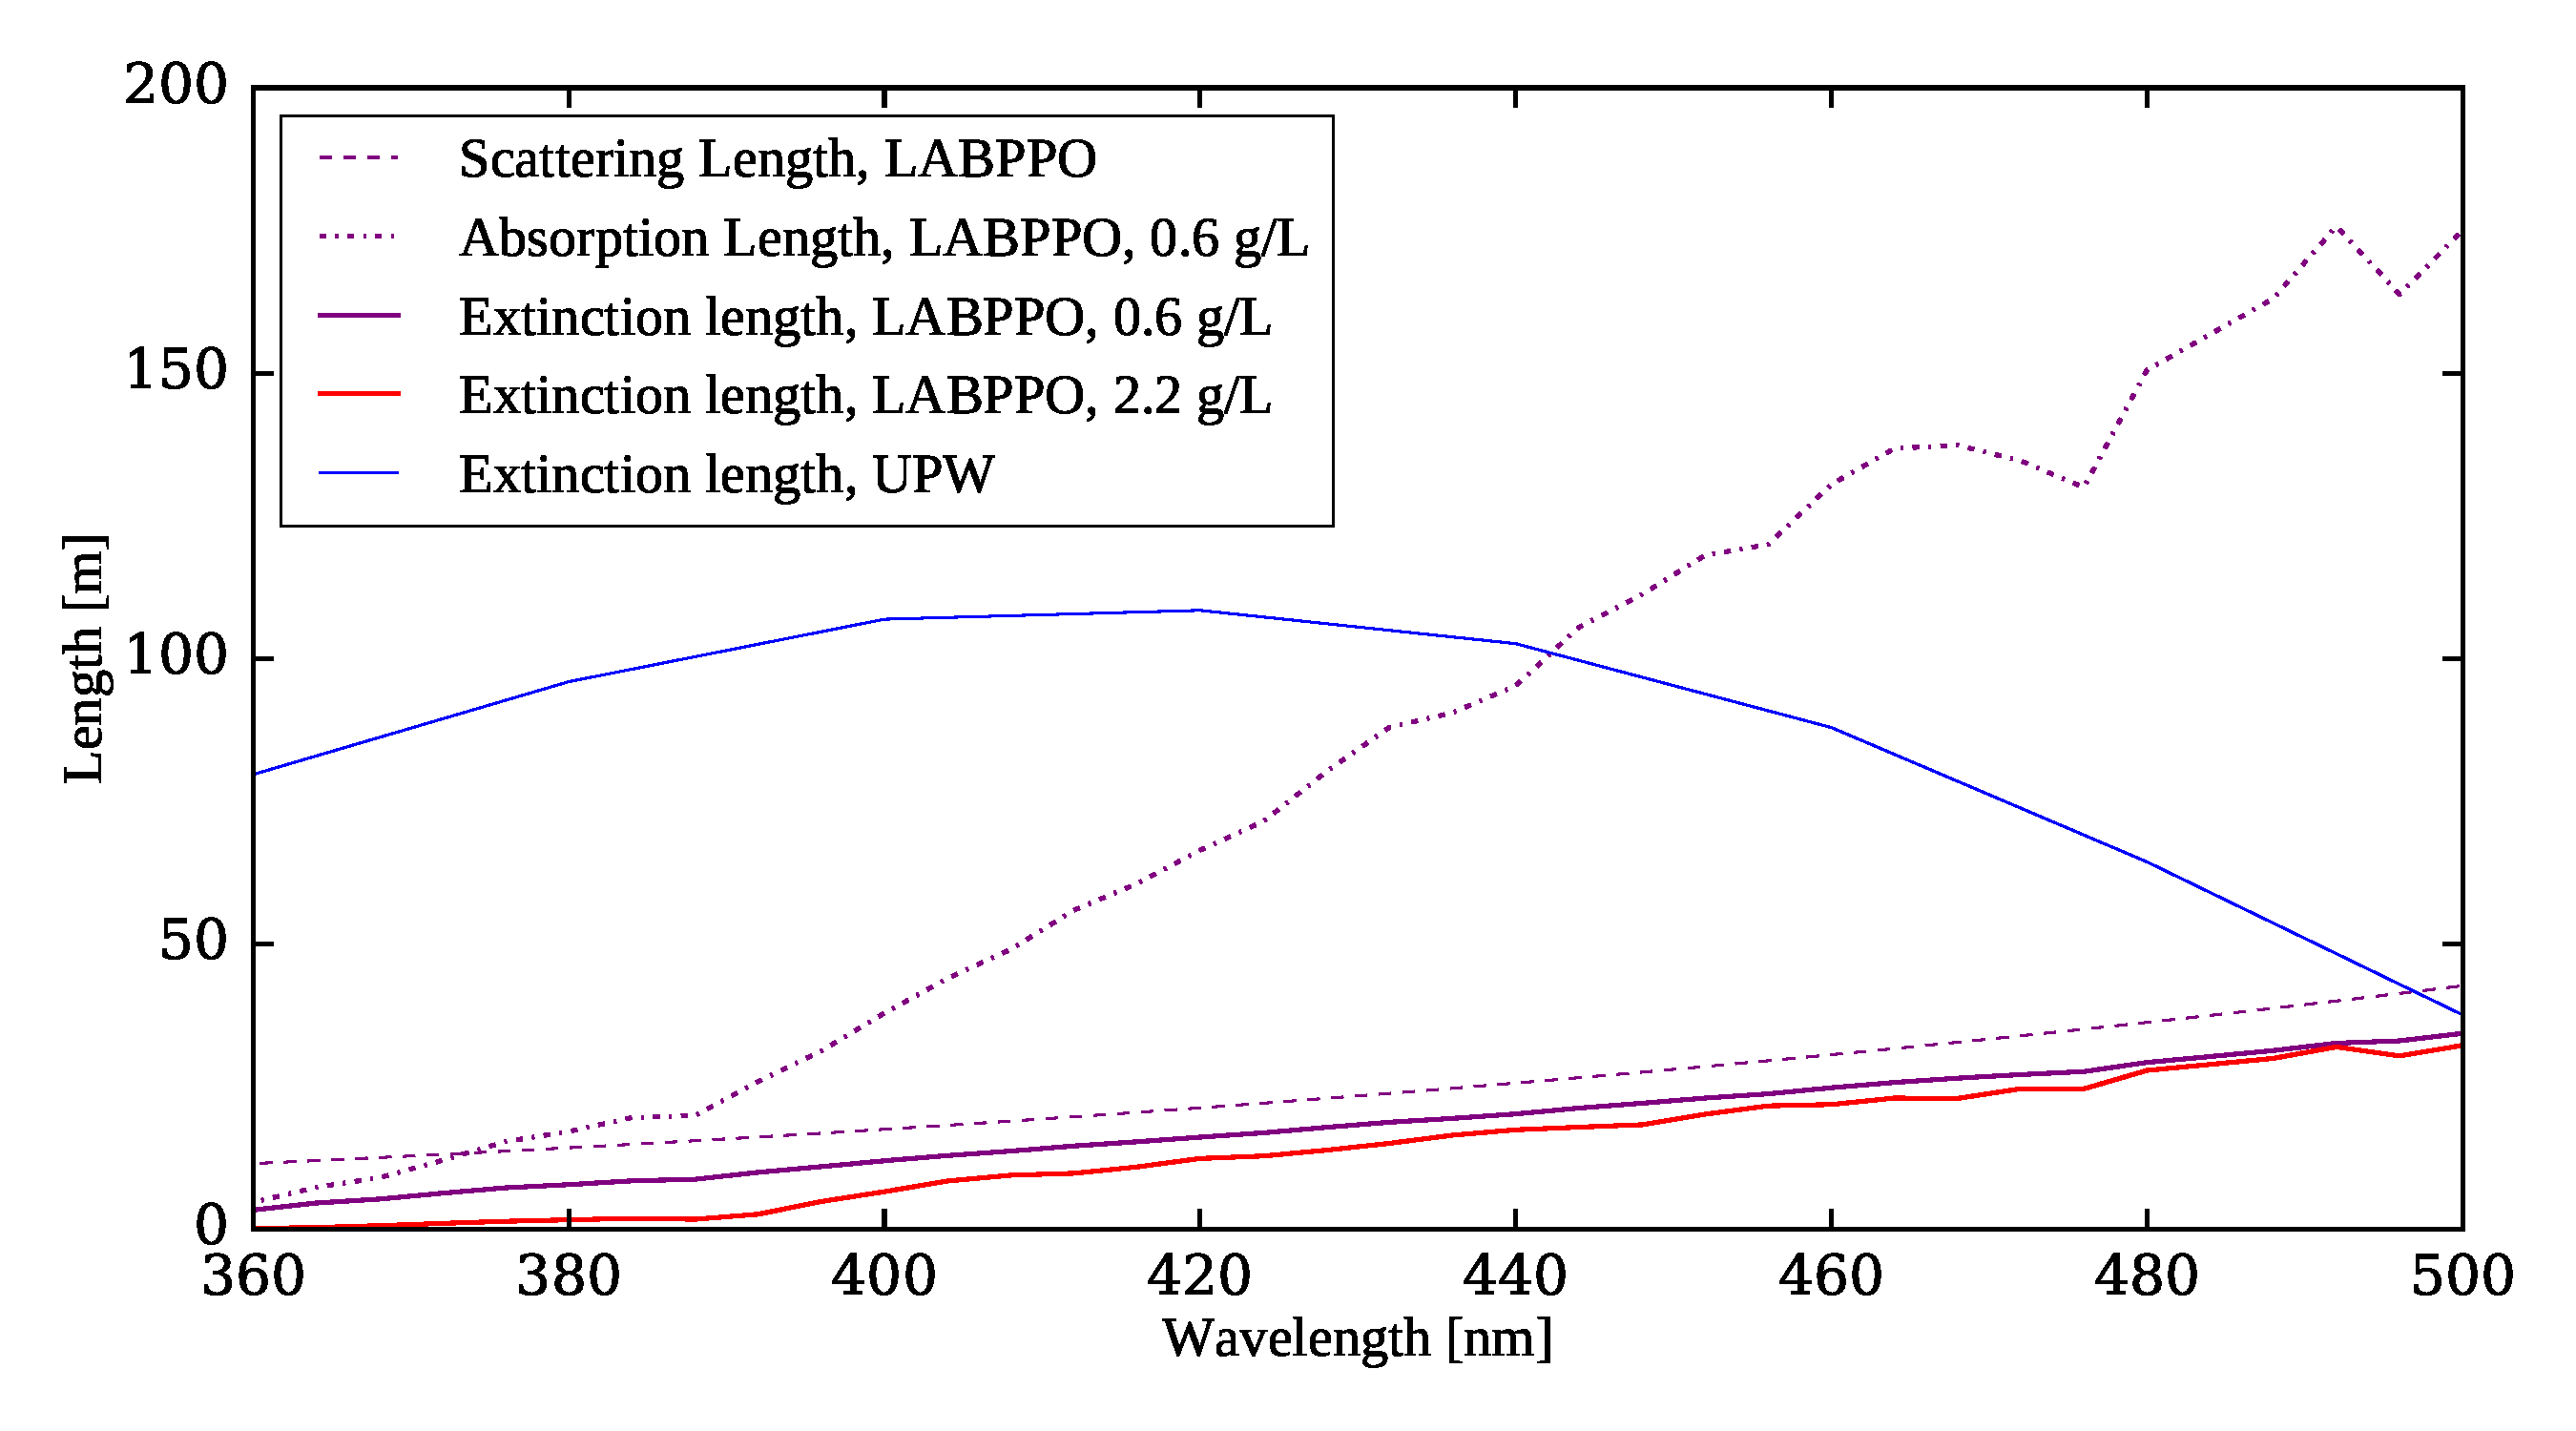
\includegraphics[width=\textwidth]{5_SMELLIEAnalysis/images/ext_length_expectations_RAT_nice.pdf}
    \caption[Current \texttt{RAT} models for the extinction lengths of both UPW and scintillator, as a function of wavelength]
    {Current \texttt{RAT} models for the extinction lengths of both UPW and scintillator, at different PPO concentrations as a function of wavelength. For the scintillator, the scattering length distribution is also shown as a dotted line, showing that it is expected for scattering to dominate over absorption in the \SIrange{400}{500}{\nm} range.}
    \label{fig:smellie_expected_ext_length_phases}
\end{figure}

\subsection{Mathematical Model}
To begin, consider light emission from a particular SMELLIE fibre of fixed wavelength $\lambda_{j}$, with a mean emission intensity of $I_{j}$ photons emitted per event in subrun $j$ during detector phase $p$. Modifying Eq.~\ref{eq:mu_def}, a general PMT $i$ will have a mean npe per event of $\mu_{ij,p}(\lambda_{j}) = I_{j,p}b_{i,p}(\lambda_{j})f_{i,p}(\lambda_{j})$. A detector phase-dependence has been added to all terms, because:
\begin{itemize}
    \item The emission intensities chosen, $I_{j,p}$, can vary between different data-taking campaigns. These changes are due to changes in hardware (as detailed in Chapter~\ref{chap:smellie_hardware}), as well as changes in the settings used to run SMELLIE.
    \item The beam profile of a given fibre at a given wavelength is not expected to change with detector phase. However, if the refractive index of the inner detector medium changes (e.g. from the water phase to scintillator phase), then the fraction of light emitted that is pointed in the correct direction to be detected by PMT $i$, $b_{i,p}(\lambda_{j})$, \textit{can} change.
    \item In a different phase of the detector, the optics of the inner detector can change. As a result, the probability that a photon pointing in the correct direction for PMT $i$ actually makes it across the detector and generates a photoelectron, $f_{i,p}(\lambda_{j})$, can change.
\end{itemize}

\begin{figure}
    \centering
    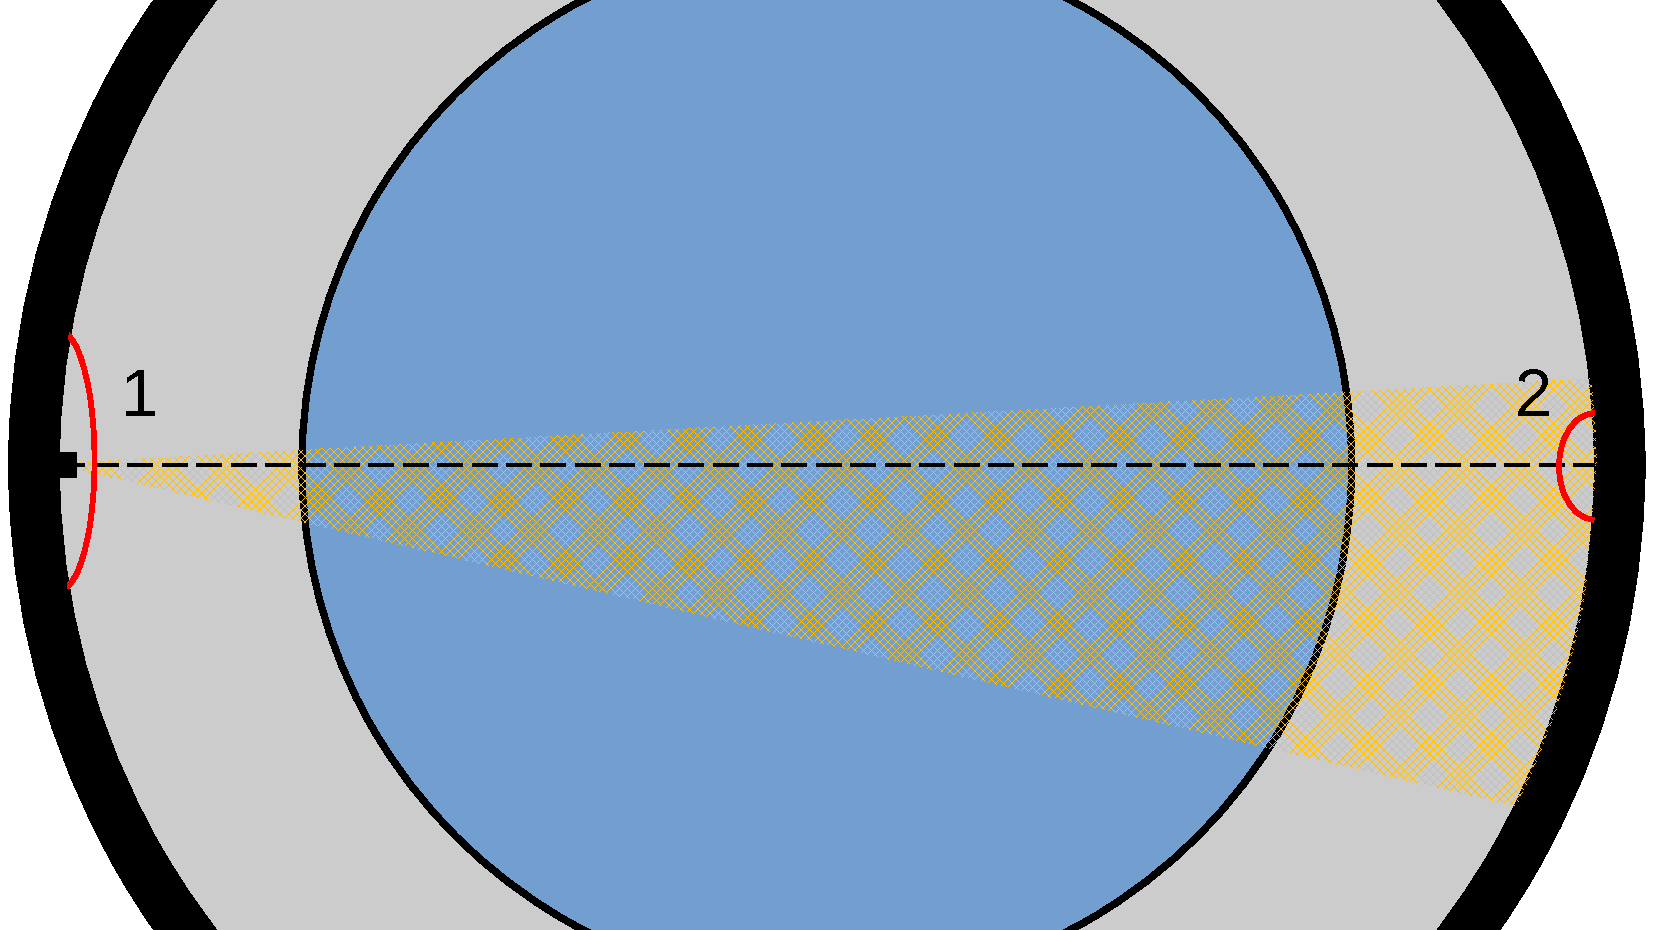
\includegraphics[width=\textwidth]{5_SMELLIEAnalysis/images/smellie_ext_length_pmt_selection_schematic.pdf}
    \caption[Diagram showing the two PMT regions used in the SMELLIE extinction length analysis]
    {Diagram showing the two PMT regions used in this analysis, indicated by red rings.}
    \label{fig:smellie_ext_length_schematic}
\end{figure}

In this analysis, two regions of PMTs will be used for a given fibre; Fig.~\ref{fig:smellie_ext_length_schematic} shows a schematic of the PMT selections. The first region corresponds to PMTs \textit{radially-opposite} the fibre emission point in the detector, i.e. the lightpaths travel orthogonally through all surface boundaries. The reason for this choice will be explained shortly. Considering the various contributions to the value of $f_{i,p}(\lambda_{j})$, a PMT in this `far' selection will have a mean npe per event, $\mu_{ij,p}^{\mathrm{far}}(\lambda_{j})$, of:
\begin{align}\label{eq:smellie_ext_length_theory}
    \mu_{ij,p}^{\mathrm{beam}}(\lambda_{j}) &= I_{j,p}b_{i,p}(\lambda_{j})
    \exp\left(
        -\frac{L_{ij,p}^{\mathrm{extern}}(\lambda_{j})}{l^{\mathrm{extern}}(\lambda_{j})}
    \right)
    \exp\left(
        -\frac{L_{ij,p}^{\mathrm{acr}}(\lambda_{j})}{l^{\mathrm{acr}}(\lambda_{j})}
    \right)
    \exp\left(
        -\frac{L_{ij,p}^{\mathrm{inner}}(\lambda_{j})}{l_{p}^{\mathrm{inner}}(\lambda_{j})}
    \right)\nonumber\\
    & \qquad\cdot T_{ij,p}(\lambda_{j})\epsilon_{ij,p}(\lambda_{j}).
\end{align}
Here, $L_{ij,p}^{\mathrm{extern,acr,inner}}(\lambda_{j})$ is the length of a path in a given detector medium through which light travels, for the external water, acrylic, and inner detector medium, respectively. $l_{p}^{\mathrm{extern,acr,inner}}(\lambda_{j})$ is the extinction length of each detector medium for a given wavelength --- it is assumed that only the inner detector medium has changing optics in different phases. Some fraction of light is lost when passing between two mediums with different refractive indices: this is captured by $T_{ij,p}(\lambda_{j})$, the product of the Fresnel transmission components for all optical boundaries along a photon's path. Finally, $\epsilon_{ij,p}(\lambda_{j})$ is the probability that a photon along a given path, incident on a given PMT, will generate a photoelectron that is detected. 

The second selection of PMTs are those near the fibre emission point. The first light observed by these PMTs will be from photons which have `back-scattered' in the UPW outside the AV. This is followed by light reflected off of the AV surface. The details of isolating this backscattered light is discussed in Section~\ref{sec:smellie_ext_length_params_and_uncs}. Assuming that the Rayleigh scattering properties of the UPW outside the AV have been unchanged throughout the lifetime of the detector, then the expected number of photoelectrons observed in a selection of these PMTs during a time period in which only back-scattering can occur will be simply:
\begin{equation}
    \mu_{j,p}^{\mathrm{back}} = kI_{j,p}.
\end{equation}
$k$ here is just some general constant of proportionality. Therefore, observing this back-scattered light can be used as a measure of the relative intensity of the subrun.

Because $\mu_{j,p}^{\mathrm{back}}$ is proportional to the intensity, the ratio $R_{ij,p} = \mu_{ij,p}^{\mathrm{beam}}(\lambda_{j})/\mu_{j,p}^{\mathrm{back}}$ will be independent of $I_{j,p}$. A similar trick can be used to remove the dependence of $R_{ij,p}$ on $k$, by taking the ratio of $R_{ij,p}$ with $R_{ij,\ce{H_{2}O}}$, where $R_{ij,\ce{H_{2}O}}$ is the measured values of $R_{ij,p}$ in the water phase. This ratio becomes:
\begin{align}
    \frac{R_{ij,p}}{R_{ij,\ce{H_{2}O}}}(\lambda_{j}) 
    &= \frac{k}{k}
    \frac{b_{i,p}(\lambda_{j})}{b_{i,\ce{H_{2}O}}(\lambda_{j})}
    \frac{T_{ij,p}(\lambda_{j})}{T_{ij,\ce{H_{2}O}}(\lambda_{j})}
    \frac{\epsilon_{ij,p}(\lambda_{j})}{\epsilon_{ij,\ce{H_{2}O}}(\lambda_{j})}
    \exp\left(
        -\frac{L_{ij,p}^{\mathrm{extern}}(\lambda_{j})-L_{ij,\ce{H_{2}O}}^{\mathrm{extern}}(\lambda_{j})}{l^{\mathrm{extern}}(\lambda_{j})}
    \right)
    \nonumber\\
    & \quad \cdot \exp\left(
        -\frac{L_{ij,p}^{\mathrm{acr}}(\lambda_{j})-L_{ij,\ce{H_{2}O}}^{\mathrm{acr}}(\lambda_{j})}{l^{\mathrm{acr}}(\lambda_{j})}
    \right)
    \exp\left(
        -\frac{L_{ij,p}^{\mathrm{inner}}(\lambda_{j})}{l_{p}^{\mathrm{inner}}(\lambda_{j})}
        +\frac{L_{ij,\ce{H_{2}O}}^{\mathrm{inner}}(\lambda_{j})}{l_{\ce{H_{2}O}}^{\mathrm{inner}}(\lambda_{j})}
    \right)
    \nonumber\\
    &= \frac{b_{i,p}(\lambda_{j})\epsilon_{ij,p}(\lambda_{j})}{b_{i,\ce{H_{2}O}}(\lambda_{j})\epsilon_{ij,\ce{H_{2}O}}(\lambda_{j})}
    \frac{T_{ij,p}(\lambda_{j})}{T_{ij,\ce{H_{2}O}}(\lambda_{j})}
    \exp\left(
        -\frac{L_{ij,p}^{\mathrm{inner}}(\lambda_{j})}{l_{p}^{\mathrm{inner}}(\lambda_{j})}
        +\frac{L_{ij,\ce{H_{2}O}}^{\mathrm{inner}}(\lambda_{j})}{l_{\ce{H_{2}O}}^{\mathrm{inner}}(\lambda_{j})}
    \right),
\end{align}
where it has been assumed that any change in path length through the external UPW or acrylic relative to their extinction lengths is negligible.

Importantly, when considering the first PMT selection, a further simplification can be made to the above formula. Because the light travels orthogonally through the AV boundaries, its path is unaffected by changes in the refractive index of the inner detector medium. Therefore, the impact of the beam profile and PMT efficiency will be unchanged, and so the formula simplifies to:
% \begin{equation}\label{eq:smellie_ext_length_rsrw_formula_1PMT}
%     R_{ij,p}(\lambda_{j}) = 
%     \frac{T_{ij,p}(\lambda_{j})}{T_{ij,\ce{H_{2}O}}(\lambda_{j})}
%     \exp\left(
%         -\frac{L_{ij,p}^{\mathrm{inner}}(\lambda_{j})}{l_{p}^{\mathrm{inner}}(\lambda_{j})}
%         +\frac{L_{ij,\ce{H_{2}O}}^{\mathrm{inner}}(\lambda_{j})}{l_{\ce{H_{2}O}}^{\mathrm{inner}}(\lambda_{j})}
%     \right)
%     \cdot R_{ij,\ce{H_{2}O}}(\lambda_{j}).
% \end{equation}
\begin{equation}\label{eq:smellie_ext_length_rsrw_formula_1PMT}
    R_{ij,\ce{H_{2}O}}(\lambda_{j}) = 
    \frac{T_{ij,\ce{H_{2}O}}(\lambda_{j})}{T_{ij,p}(\lambda_{j})}
    \exp\left(
        \frac{L_{ij,p}^{\mathrm{inner}}(\lambda_{j})}{l_{p}^{\mathrm{inner}}(\lambda_{j})}
        -\frac{L_{ij,\ce{H_{2}O}}^{\mathrm{inner}}(\lambda_{j})}{l_{\ce{H_{2}O}}^{\mathrm{inner}}(\lambda_{j})}
    \right)
    \cdot  R_{ij,p}(\lambda_{j}).
\end{equation}
The measurable quantities $R_{ij,\ce{H_{2}O}}(\lambda_{j})$ and $R_{ij,p}(\lambda_{j})$ are then proportional to one another, with the constant of proportionality being a function of the variable of interest $l_{p}^{\mathrm{inner}}(\lambda_{j})$.

% Rearranging the above for $l_{p}^{\mathrm{inner}}(\lambda_{j})$, one can write:
% \begin{align}\label{eq:smellie_ext_length_1PMT}
%     l_{p}^{\mathrm{inner}}(\lambda_{j}) &= 
%     \frac{
%         L_{ij,p}^{\mathrm{inner}}(\lambda_{j})
%         }{
%         \ln\left(
%             \frac{R_{ij,\ce{H_{2}O}}}{R_{ij,p}}(\lambda_{j})\cdot s_{ij,p}(\lambda_{j})
%         \right)
%         + \ln\left(
%             \frac{T_{ij,p}(\lambda_{j})}{T_{ij,\ce{H_{2}O}}(\lambda_{j})}
%         \right)
%         + \frac{L_{ij,\ce{H_{2}O}}^{\mathrm{inner}}(\lambda_{j})}{l_{\ce{H_{2}O}}^{\mathrm{inner}}(\lambda_{j})}
%     },\nonumber\\
%     s_{ij,p}(\lambda_{j}) &=
%     \frac{
%         b_{i,\ce{H_{2}O}}(\lambda_{j})\epsilon_{ij,\ce{H_{2}O}}(\lambda_{j})
%         }{
%         b_{i,p}(\lambda_{j})\epsilon_{ij,p}(\lambda_{j})
%     }.
% \end{align}
% The parameter $s_{ij,p}(\lambda_{j})$ describes the fractional change in observed npe for a given PMT due to differences in refraction between the phases. Quantifying this effect will be discussed in Section~\ref{sec:smellie_ext_corrections}.

\subsection{Parameter Measurements and Uncertainties}\label{sec:smellie_ext_length_params_and_uncs}
As a result of Eq.~\ref{eq:smellie_ext_length_rsrw_formula_1PMT}, measuring the extinction length of the scintillator requires first measuring a number of other quantities with knowledge of their uncertainties.

\subsubsection{UPW Extinction Lengths}
As discussed in Section~\ref{sec:optical_processes}, the attenuation lengths of the UPW were measured as a function of wavelength in the water phase with the Laserball. It is assumed that the optics of the UPW inside and outside the AV were the same, and outer UPW has not changed since.

In this analysis, the measured values of the attenuation coefficients $\alpha_{w}(\lambda) = 1/l_{\ce{H_{2}O}}^{\mathrm{inner}}(\lambda)$ and their associated errors were taken from~\cite{andersonOpticalCalibrationSNO2021}. The wavelength range this Laserball data was taken over was \SIrange{337}{500}{\nm}, so avoid extrapolation only wavelengths in this range were considered in this analysis. For a given SMELLIE subrun with wavelength $\lambda_{j}$, $l_{\ce{H_{2}O}}^{\mathrm{inner}}(\lambda_{j})$ was estimated by linearly interpolating between Laserball $\alpha_{w}$ data points, and then taking a reciprocal. Because the systematic uncertainties dominated for each Laserball data point, which were likely to be highly correlated between data points, the uncertainty in $\alpha_{w}(\lambda_{j})$ was estimated by linearly interpolating the quadrature sum of the statistical and systematic uncertainties at each Laserball data point. Fig.~\ref{fig:smellie_laserball_water_ext_length_est} shows this process in action from the wavelength \SI{375}{\nm}. At its largest, the uncertainty in $l_{\ce{H_{2}O}}^{\mathrm{inner}}$ is $\sim50\%$. Fortunately, the impact of this large error is mitigated in Eq.~\ref{eq:smellie_ext_length_rsrw_formula_1PMT} because $L_{ij,\ce{H_{2}O}}^{\mathrm{inner}}(\lambda_{j})\ll l_{\ce{H_{2}O}}^{\mathrm{inner}}$.

\begin{figure}
    \centering
    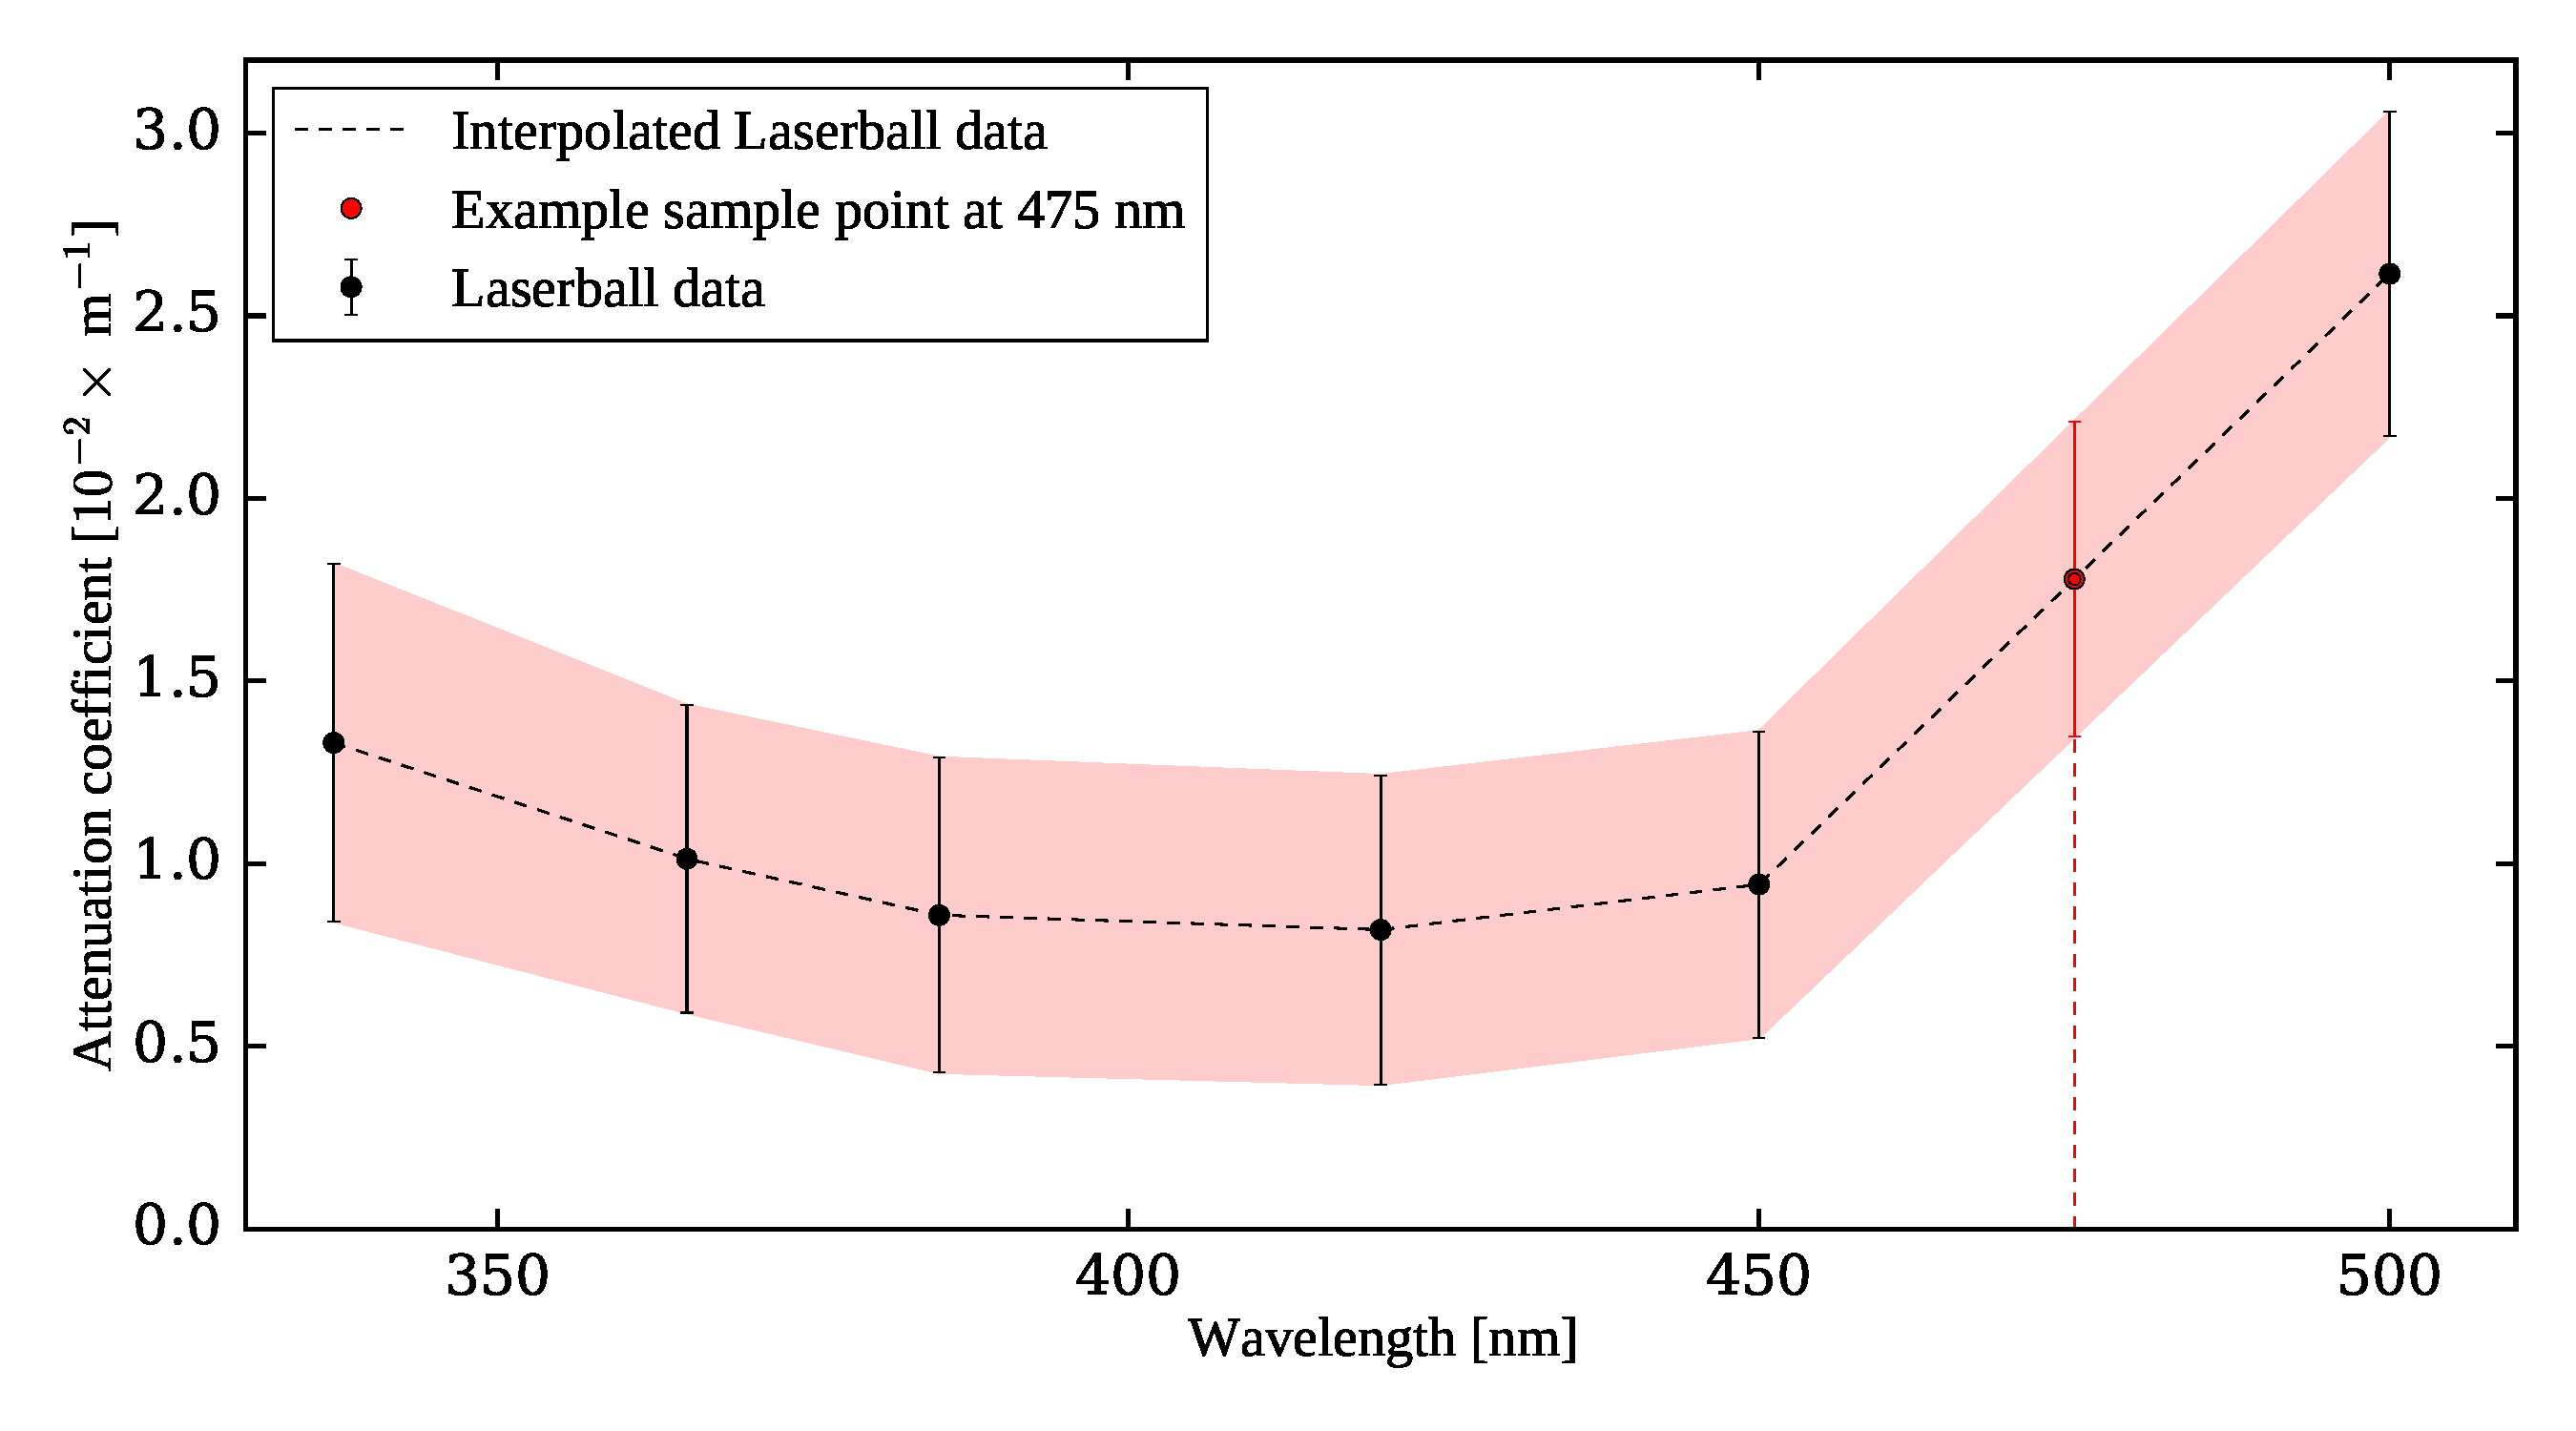
\includegraphics[width=\textwidth]{5_SMELLIEAnalysis/images/OCA_water_atten_coeffs_with_interploation.pdf}
    \caption[Linear interpolation being used on Laserball UPW attenuation coefficient data]
    {Plot showing how linear interpolation has been used on the Laserball water phase UPW attenuation coefficient data. An example point at \SI{475}{\nm} is shown explicitly.}
    \label{fig:smellie_laserball_water_ext_length_est}
\end{figure}

\subsubsection{Path Lengths and Transmission Coefficients}
Section~\ref{sec:optical_processes} also discusses the measured refractive indices as a function of wavelength for the UPW, acrylic, and LABPPO. For a given detector phase, subrun, and PMT, the Collaboration's \texttt{Light Path Calculator} is able to determine the values of $L_{ij,p}^{\mathrm{inner}}(\lambda_{j})$ as well as the combined Fresnel transmission coefficient $T_{ij,p}(\lambda_{j})$. It is assumed that there is negligible uncertainty in these values.

\subsubsection{Measuring the Number of Photoelectrons}
Critical to this analysis is the determination of the mean npe per event in both `far' and `backscatter' PMTs. These two PMT selections have to be approached slightly differently.

The `far' PMTs were selected by first finding the intersection point on the PSUP with a line that passes through both the fibre emission point and the centre of the AV. The 20 PMTs closest to this point were chosen. For a given analysis between a scintillator phase subrun $j$ and a matching water phase subrun, only PMTs inside this selection which were identified as ``good'' (as defined in Section~\ref{sec:combining_beam_profiles}) in both subruns were used. For a given far PMT being used, direct light was isolated by calculating the time residuals of all hits on the PMT, using the ``$t_{\mathrm{emm}} = t_{\mathrm{med}}$'' approach mentioned in Section~\ref{sec:smellie_triggering_daq}. Then, the number of hits observed in a ``tight'' time residual window of $[-5,+5]\,\si{\ns}$ was measured for the PMT of interest. By converting to occupancy and then using a multi-hit correction as described in Eq.~\ref{eq:multihit_correction}, the total npe per event for that PMT was estimated. The uncertainty in this value was given by the Poisson error of the calculated npe. In order to minimise the statistical uncertainty, all individual far npe measurements for a given subrun were combined into one value of the `far' light npe per event, $\mu_{j,p}^{\mathrm{far}}$.

Backscattered PMTs were selected for each fibre by finding the 50 PMTs closest to the fibre emission point. A \tres{} window of $[-30,-10]\,\si{\ns}$ was used for the isolation of backscattered light in each subrun. Like above, the total hits for each PMT was converted into a total npe with associated Poisson error. A final correction was made to account for noise hits: the measured noise rate of a given PMT was calculated using the PULSEGT triggers, as described in Section~\ref{sec:smellie_software}. After accounting for the width of the time window, the corresponding expected number of noise hits was subtracted off of the total measured npe to give the npe per event from direct light only. The npe from these PMTs were combined into one value of the backscattered light npe per event, $\mu_{j,p}^{\mathrm{back}}$. The variables $R_{s}$ and $R_{w}$ are the ratios of the far light npe to the backscattered light npe for a given scintillator or water phase subrun, respectively. The subrun $j$ subscript has been dropped for simplicity.

Fig.~\ref{fig:smellie_extlength_PMT_selections} shows the time residual distributions for both PMT selections of a simulation of the PQ407 laser being fired through fibre FS007 during the scintillator phase, with \SI{2.2}{\gpl} PPO loading. The simulation used the optical model described in Section~\ref{sec:optical_processes}. The earliest photon track associated with a given PMT hit was classified by the optical processes it underwent. A hit associated with a photon that travelled unimpeded through the detector is classified as `direct'. For this fibre and wavelength combination, the time residual windows used allow for a signal-to-background ratio of XXX for the far PMTs, and XXX for the backscattered PMTs. % FILL IN.

\begin{figure}
    \centering
    \begin{subfigure}{0.98\textwidth}
        \centering
        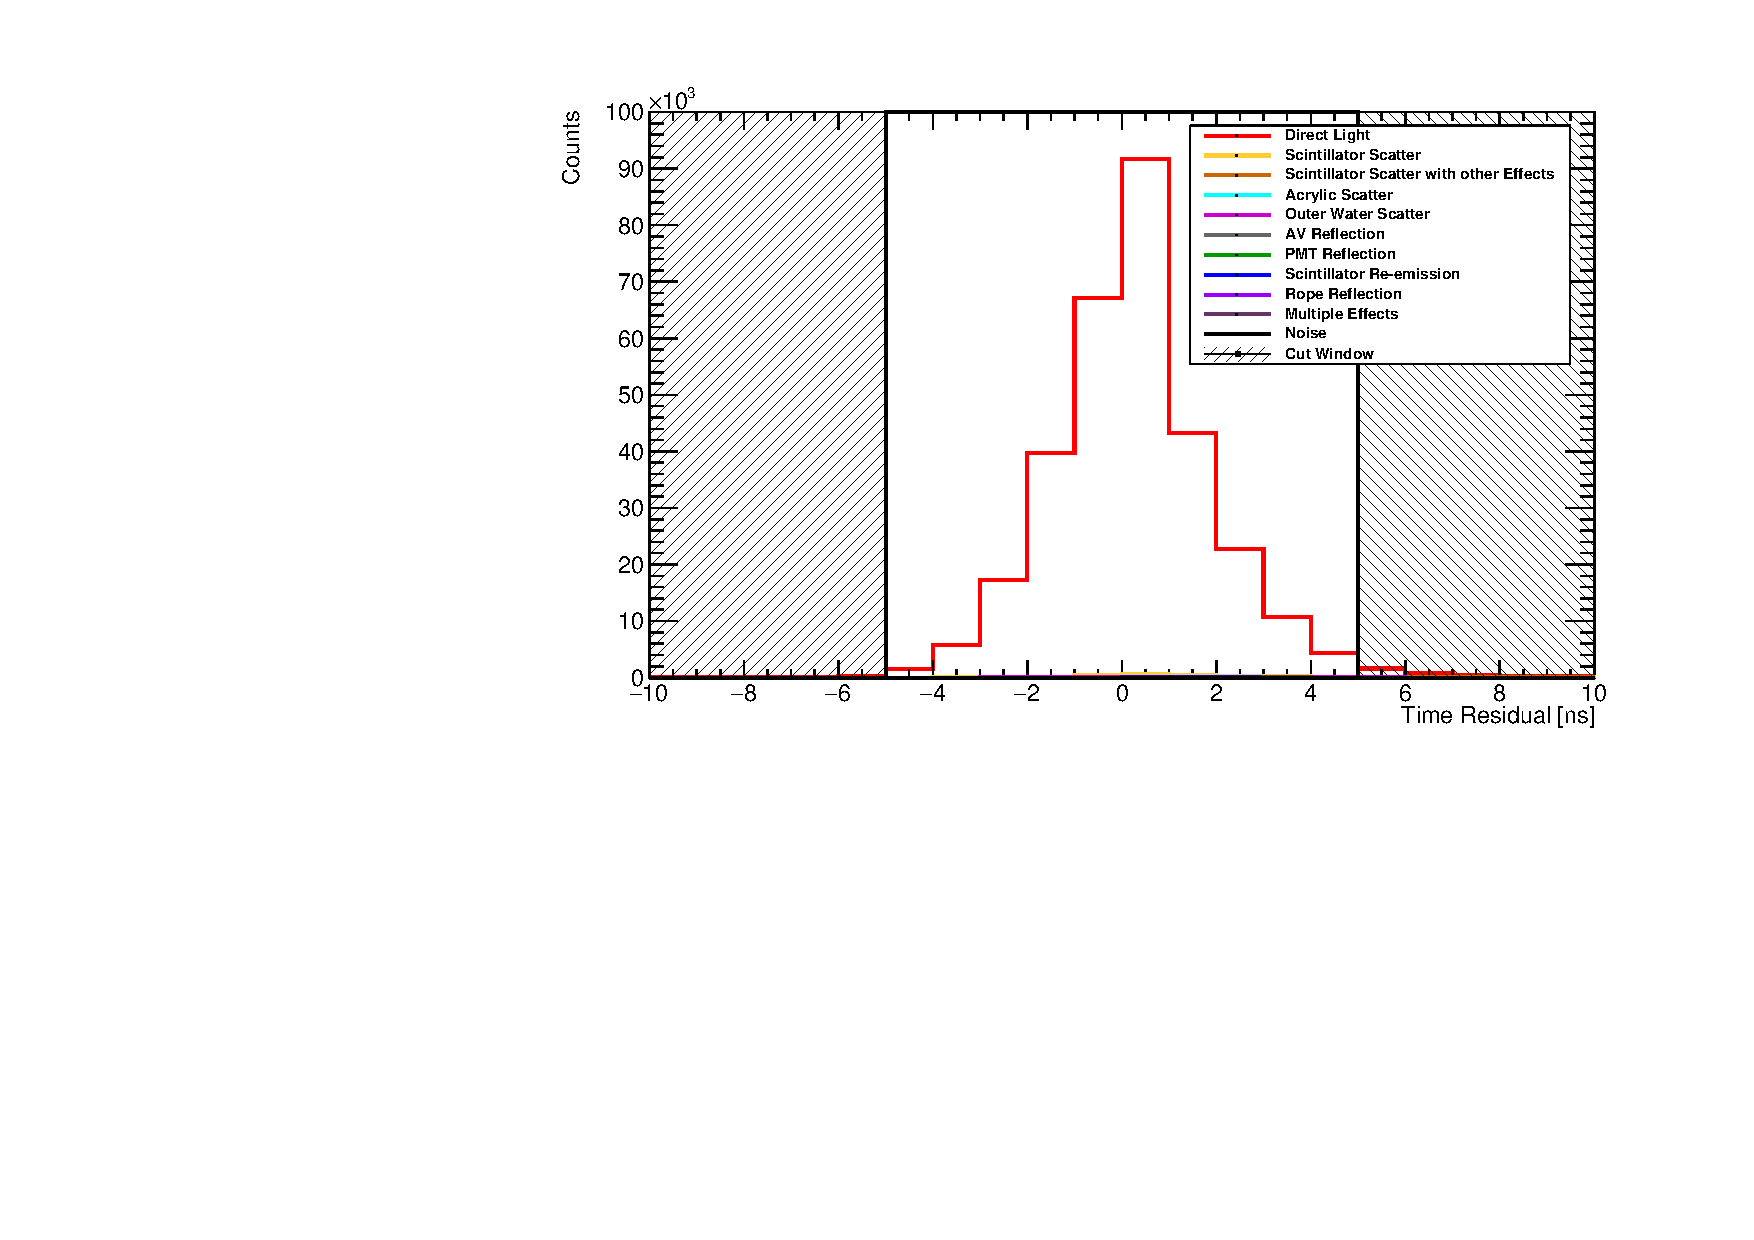
\includegraphics[width=\textwidth]{5_SMELLIEAnalysis/images/far_pmts_tres_components_nice_PQ407_FS007.pdf}
        \caption{Far region}
        \label{fig:smellie_far_PMT_selection}
    \end{subfigure}
    \begin{subfigure}{0.98\textwidth}
        \centering
        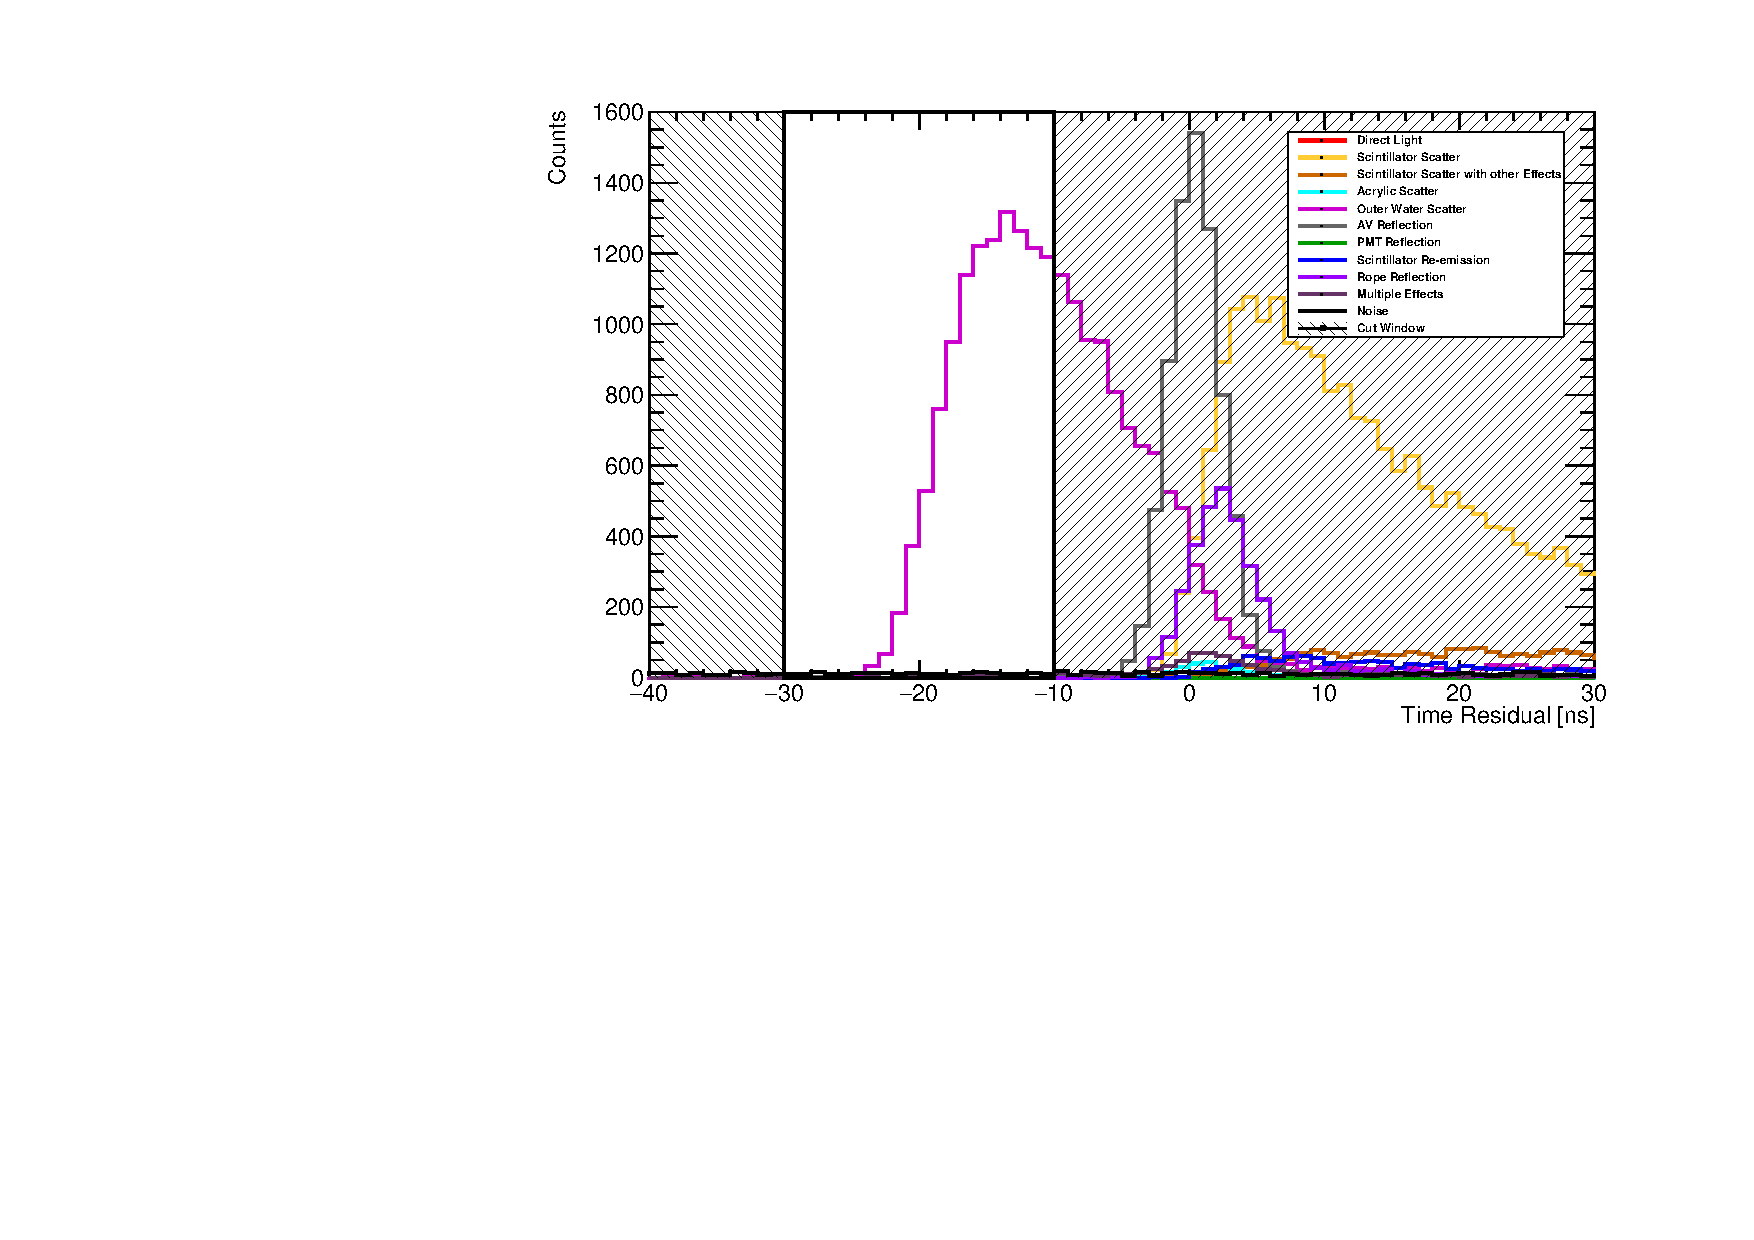
\includegraphics[width=\textwidth]{5_SMELLIEAnalysis/images/backscatter_pmts_tres_components_nice_PQ407_FS007.pdf}
        \caption{Backscatter region}
        \label{fig:smellie_backscat_PMT_selection}
    \end{subfigure}
    \caption[Time residual distributions of the far and backscatter PMT regions for a simulation using laser PQ407 through fibre FS007, split by the different optical components]
    {Time residual distributions of the far and backscatter PMT regions for a simulation using laser PQ407 through fibre FS007, split by the different optical components. The time windows defining the signal regions are shown in both.}
    \label{fig:smellie_extlength_PMT_selections}
\end{figure}

$t_{\mathrm{med}}$ was used in this analysis instead of $t_{2}$ because it was found to be far more robust to changes in emission intensity. Fig.~\ref{fig:t2_temm_comparison} shows a comparison of the \tres{} distribution for backscattered PMTs between using $t_{2}$ and $t_{\mathrm{med}}$, at different emission intensities. As can be seen, the $t_{2}$ distribution is biased towards positive \tres{} values as intensity increases. This is not the case when using $t_{\mathrm{med}}$. 

\begin{figure}
    \centering
    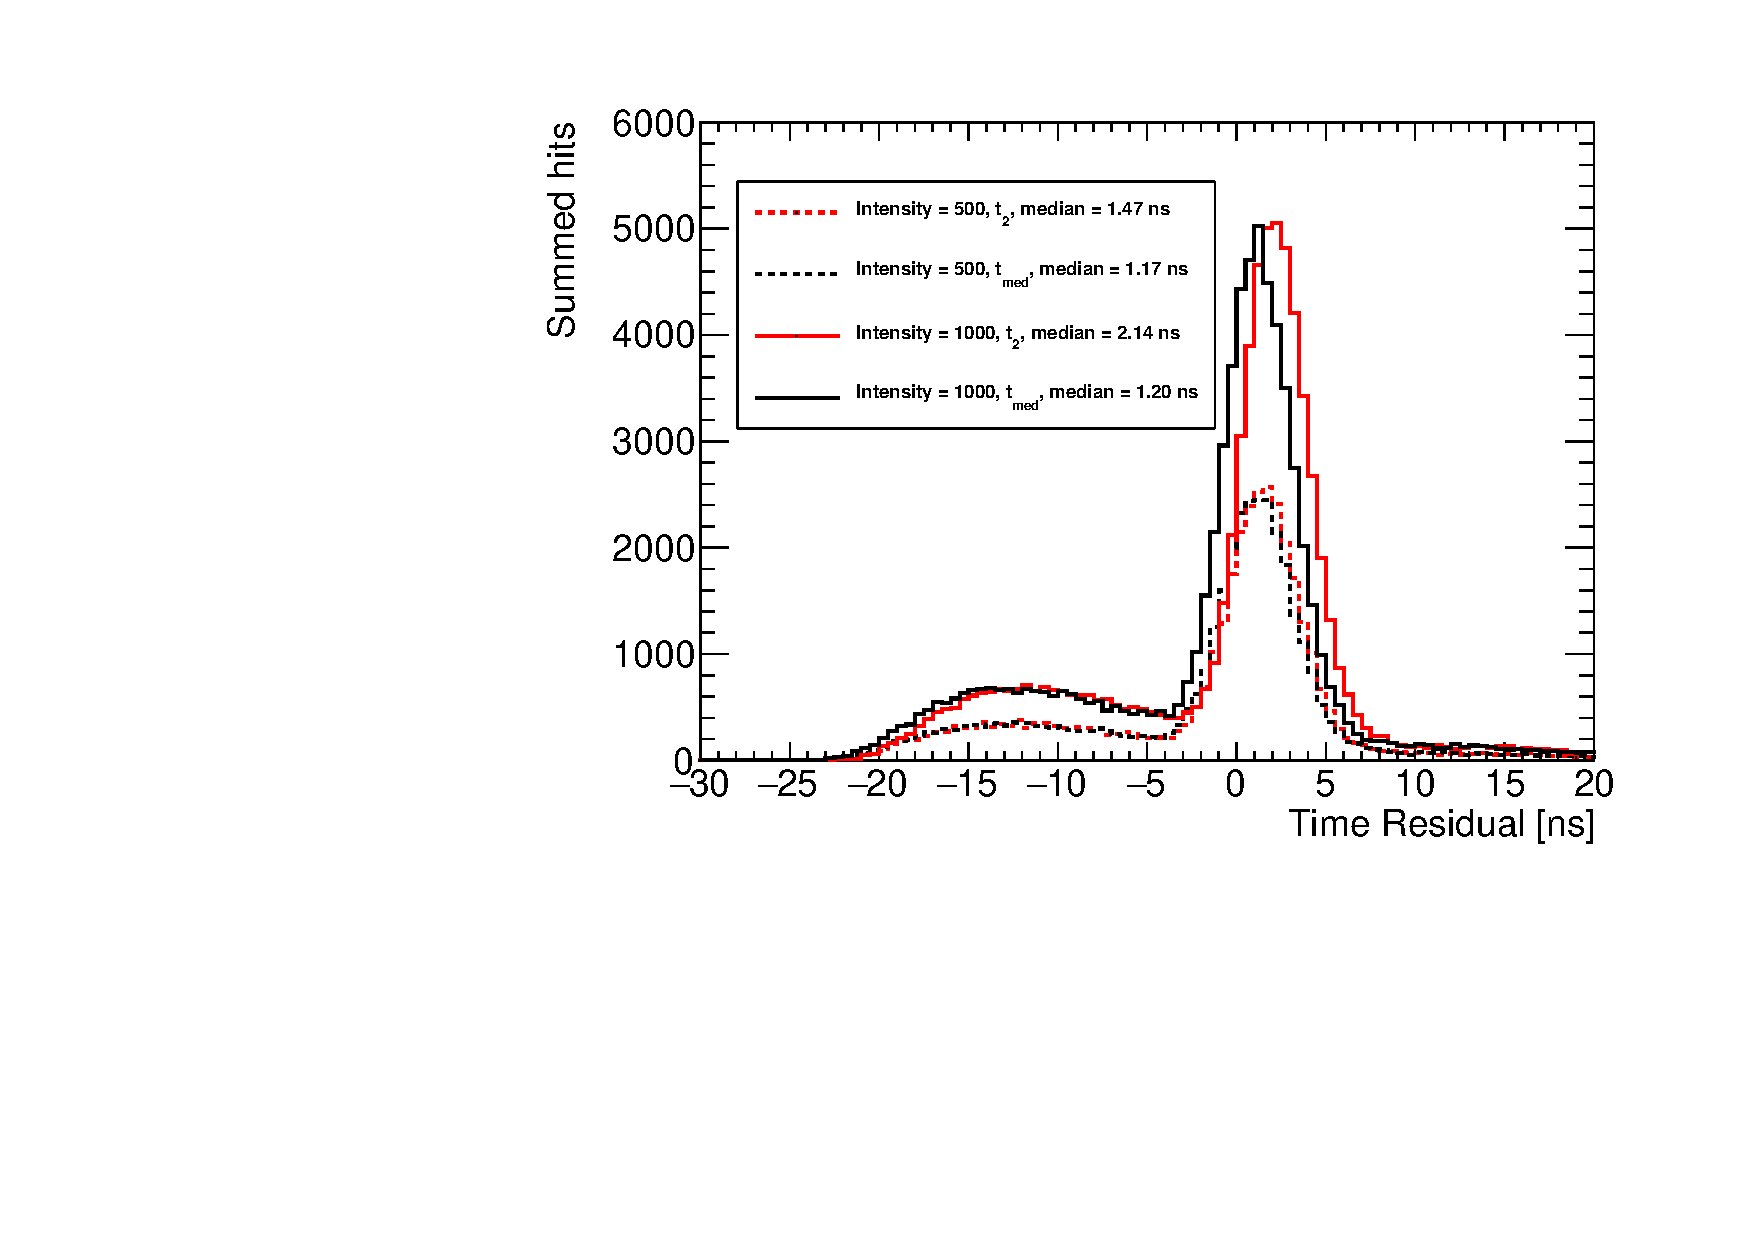
\includegraphics[width=\textwidth]{5_SMELLIEAnalysis/images/t2_vs_tmed_backscatter_region_comparison_vs_intensity.pdf}
    \caption[Comparison of the backscatter light region time residual distribution with intensity and emission time calculation choice]
    {Comparison of the backscatter light region time residual distribution, as a function of both emission intensity and emission time calculation choice. A clear intensity-dependence can be seen when using $t_{2}$, whereas $t_{\mathrm{med}}$ is much more robust.}
    \label{fig:t2_temm_comparison}
\end{figure}

% \begin{itemize}
%     \item Outline theoretical approach for how one could measure the extinction length of scintillator through a comparison of SMELLIE data between the scintillator and water phases, in the simplified 1 dimensional case with only 2 PMTs.
% \end{itemize}
% [3 pages]

% \subsubsection{Differential Beamspot Refraction}\label{sec:smellie_ext_corrections}
% The correction factor $s_{ij,p}(\lambda_{j})$ is very important for comparing water and scintillator phase data like-for-like. As the SMELLIE beam travels through the AV, refraction bends it by a small amount. However, the amount of this bending will change as a function of the refractive index of the inner detector medium. Because the beam profile drops roughly exponentially as a function of $\alpha$, even small movements in the SMELLIE beam can have a substantial impact on the measured npe for a given beamspot PMT.

% To quantify this effect, SMELLIE events were simulated under ideal conditions in the water phase for every fibre, with the PQ495 laser. Then, the npe per event in the prompt time window was calculated using the same approach described in the previous section. % CONFIRM!!
% The use of the water phase and \SI{495}{\nm} wavelength was chosen so that the impact from optical scattering or absorption would be small. Then, the refractive index of the inner water was modified to match that of LAB, and the above simulations and npe calculations were repeated. The results of this are shown for fibre FS107 in the first two plots of Fig.~\ref{fig:smellie_ref_index_ratio_beamspot}. As can be seen, there is a clear movement of the beam by a polar angle of $\sim\ang{5}$. % CONFIRM!!!
% The movement of other common features in the beamspot, such as the rope shadows and ring structures, can also be seen. There is also a dramatic band of low-npe PMTs that appears only in the latter simulation. This phenomenon will be explained and taken advantage of in Section~\ref{sec:smellie_scatt_new_method} for the scattering analysis.

% \begin{figure}
%     \centering
%     % 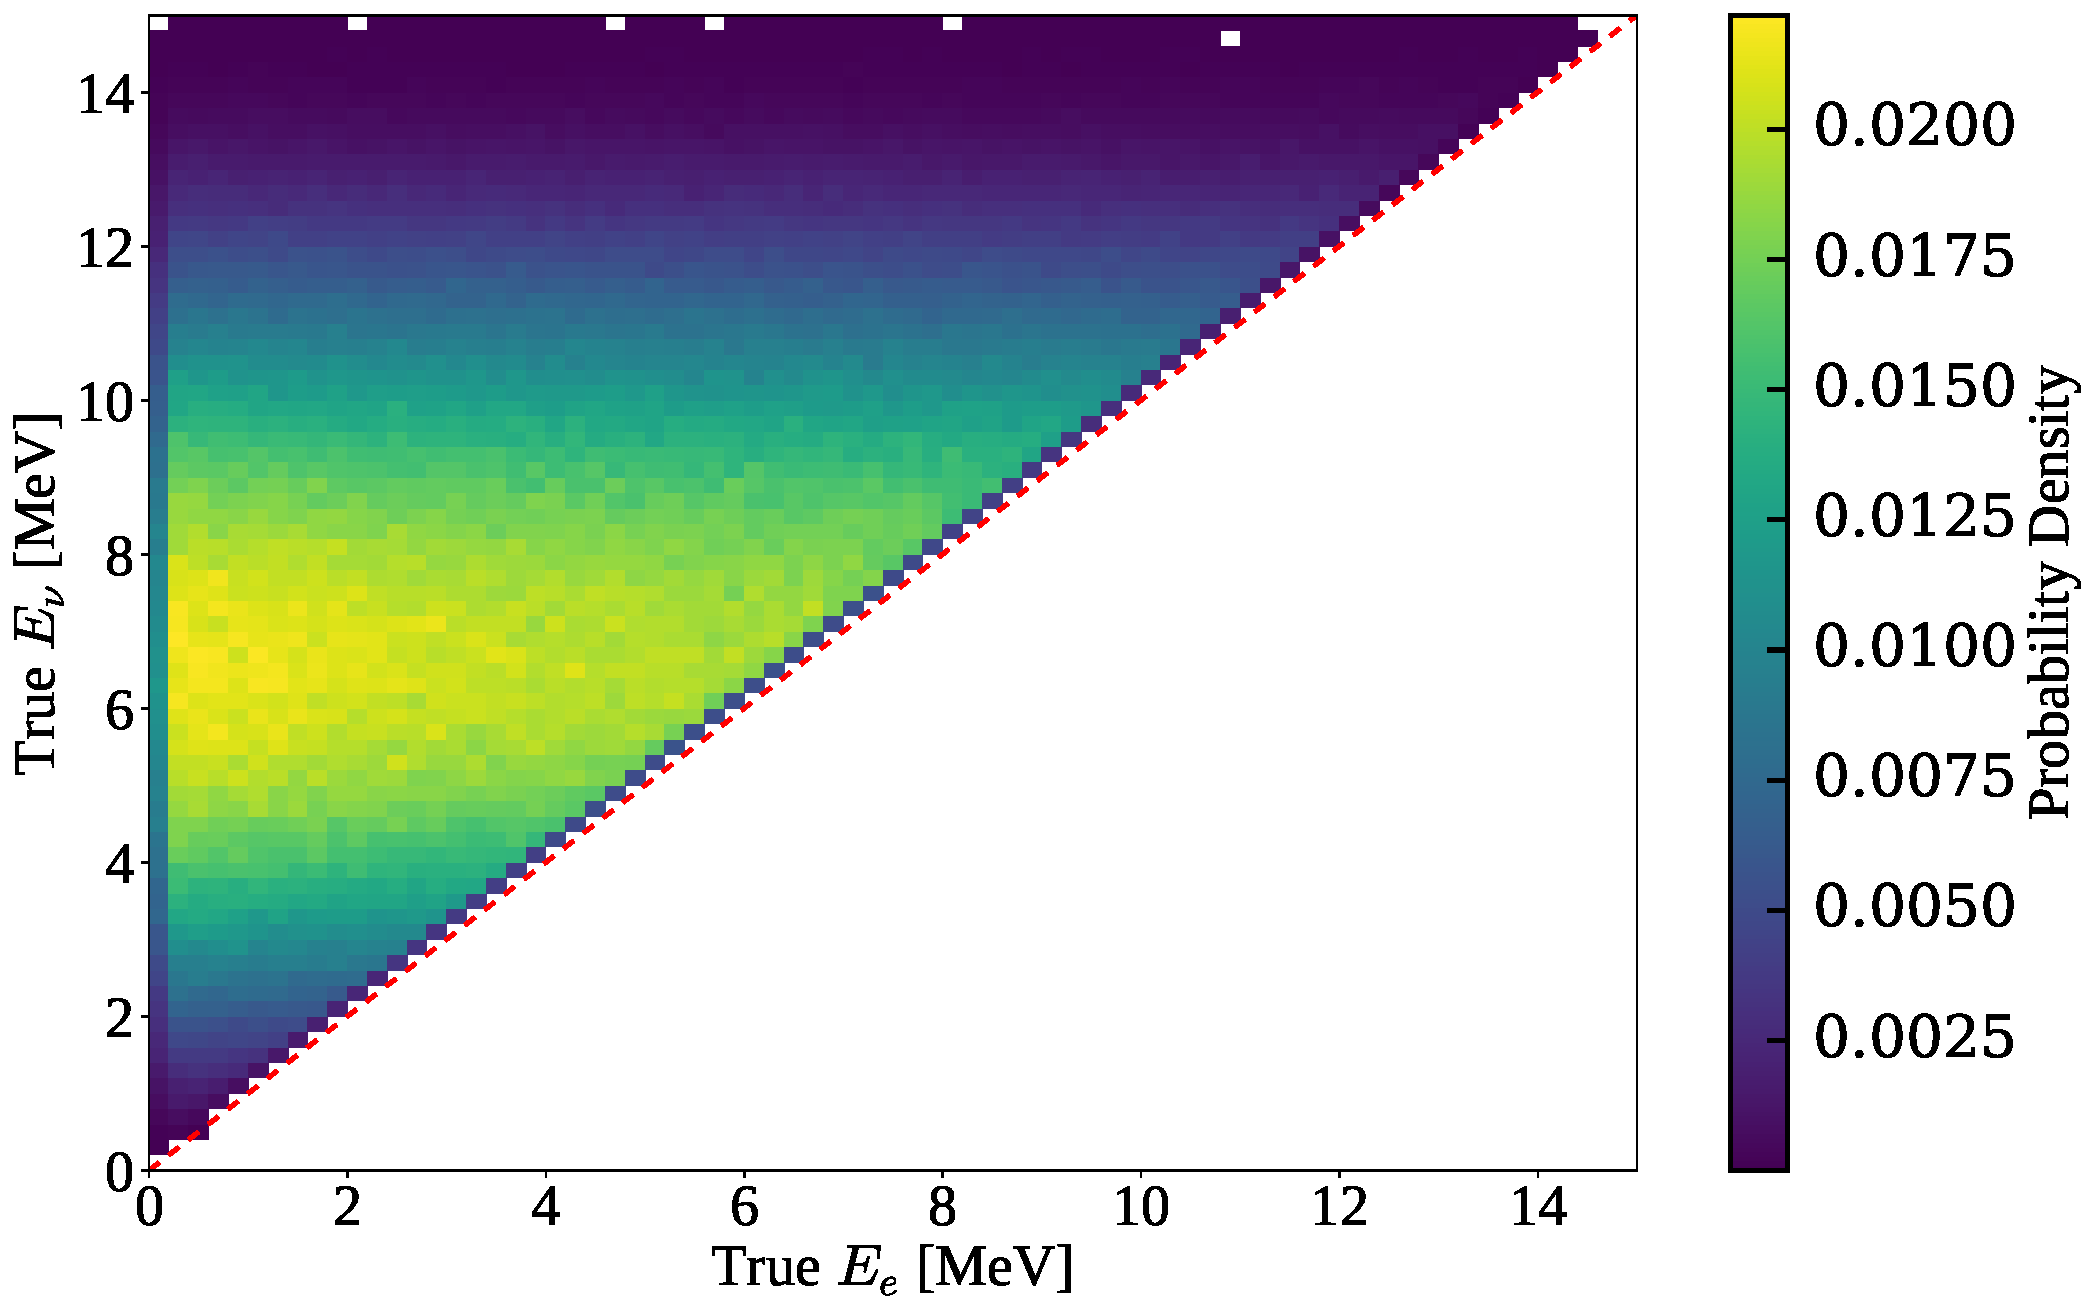
\includegraphics[width=0.8\textwidth]{6_SolarAnalysis/images/b8_eelectrue_vs_enutrue.pdf}
%     \caption[]{}
%     \label{fig:smellie_ref_index_ratio_beamspot}
% \end{figure}

% These simulations were then used to estimate the values of $s_{ij,p}(\lambda_{j})$ in the beamspot. It was assumed that the beam profiles used in simulation were a reasonable model for the beamspot, and there was no wavelength-dependence in these profiles. Assuming that the fractional changes in path lengths relative to their associated extinction lengths are negligible, by using Eq.~\ref{eq:smellie_ext_length_theory} the above ratio will just be:
% \begin{equation}
%     \frac{\mu_{ij,\ce{H_{2}O}}^{\mathrm{beam}}}{\mu_{ij,\ce{H_{2}O}'}^{\mathrm{beam}}}
%     = \frac{T_{ij,\ce{H_{2}O}}}{T_{ij,\ce{H_{2}O}'}}\cdot
%     \frac{b_{ij,\ce{H_{2}O}}\epsilon_{ij,\ce{H_{2}O}}}{b_{ij,\ce{H_{2}O}'}\epsilon_{ij,\ce{H_{2}O}'}}
%     = \frac{T_{ij,\ce{H_{2}O}}}{T_{ij,\ce{H_{2}O}'}}\cdot s_{ij,\mathrm{scint}},
% \end{equation}
% where $p = \ce{H_{2}O}'$ corresponds to the simulation with the modified refractive index. Therefore, the values of $s_{ij,\mathrm{scint}}$ can be estimated by:
% \begin{equation}
%     s_{ij,\mathrm{scint}} = 
%     \frac{\mu_{ij,\ce{H_{2}O}}^{\mathrm{beam}}}{\mu_{ij,\ce{H_{2}O}'}^{\mathrm{beam}}}
%     \cdot \frac{T_{ij,\ce{H_{2}O}'}}{T_{ij,\ce{H_{2}O}}}.
% \end{equation}

% Both the ratio $\frac{\mu_{ij,\ce{H_{2}O}}^{\mathrm{beam}}}{\mu_{ij,\ce{H_{2}O}'}^{\mathrm{beam}}}$ and the derived value for $s_{ij,\mathrm{scint}}$ for fibre FS107 are shown in Fig.~\ref{fig:smellie_ref_index_ratio_beamspot}. % ADD SOME COMMENTS HERE?? ALSO ABOUT ASSUMPTION OF BEAM PROFILE


% \begin{itemize}
%     \item Not doing analysis with just 2 PMTs, of course! Can combine results from multiple PMTs within a beamspot: I explain how here.
% \end{itemize}
% [2 pages]

% \subsubsection{Corrections Between the Water and Scintillator Phases}
% \begin{itemize}
%     \item Note the complications that we have to deal with. Namely, the differing refractive indices of the media bending the beamspot differently in the phases, as well as the method used to estimate $t_{\textrm{emm}}$.
%     \item Explain how we deal with these, the former through MC simulation.
% \end{itemize}
% [2 pages]


% \subsection{Validation of the Analysis in Simulation}
% \begin{itemize}
%     \item Show results of this approach being used to measure the extinction length in simulation. How well does it do?
% \end{itemize}
% [3 pages]

\subsection{Results in Data}
\subsubsection{Datasets Used}
The datasets used in this analysis are summarised in Table~\ref{tab:smellie_ext_length_data}. The water phase data all came from run \num{114018}; scintillator phase data was taken at five different points during the scintillator phase, two during the loading of PPO and three afterwards. These datasets match those highlighted in Fig.~\ref{fig:smellie_timeline}.

\begin{table}
    \begin{center}
        \begin{tabulary}{\textwidth}{c L L}
            \hline
            Date & Detector Phase & Runs used \\ \hline \hline
            June 2018 & Water Phase & \num{114018} \\ \hline
            May 2021 & Scintillator Phase, \SI{0.6}{\gpl} PPO & \num{270856}, \num{270857}, \num{270858}, \num{270862} \\
            October 2021 & Scintillator Phase, \SI{1.1}{\gpl} PPO & \num{275674}; \num{275676}; \num{275678}; \num{275680} \\
            May 2022 & Scintillator Phase, \SI{2.2}{\gpl} PPO & \num{300706}; \num{300708}; \num{300710}; \num{300712}; \num{300715}; \num{300748} \\
            July 2022 & Scintillator Phase, \SI{2.2}{\gpl} PPO & \num{302628}; \num{302630}; \num{302632}; \num{302634}; \num{302636} \\
            June 2023 & Scintillator Phase, \SI{2.2}{\gpl} PPO & \num{310292}; \num{310294}; \num{310296}; \num{310298}; \num{310303} \\\hline
        \end{tabulary}
    \end{center}
    \caption[Datasets used in this analysis]
    {Datasets used in this analysis.}
    \label{tab:smellie_ext_length_data}
\end{table}

`Medium' intensity subruns from the PQ407, PQ495, and SuperK lasers were used in this study. Results from the PQ446 laser are not shown, as many extinction length values produced were unphysical, likely due to the very substantial intensity instabilities seen in much of their water and scintillator phase subruns. The PQ375 laser was also not used, for reasons discussed shortly. Fibres FS193 and FS293 were not used as they failed to ever allow a substantial amount of light through them; FS207 was also not used as there was no beam profile distribution made for that fibre. Every scintillator phase subrun being used was matched to an equivalent water phase subrun.

The sensitivity of the extinction length measurement is strongly dependent on the ratio of that extinction length to the length scale of the AV. Very long extinction lengths are difficult to measure because only a small amount of light is expected to be lost due to scattering or absorption. In contrast, at short extinction lengths only a very small amount of light will reach the other side without being extinguished; the dominant source of hits will come from scattered or re-emitted light.

As an example, Fig.~\ref{fig:smellie_PQ375_far_pmts_components} shows the expected optical component breakdown for hits from far PMTs from fibre FS007 due to laser PQ375, using the current \texttt{RAT} model of the \SI{2.2}{\gpl} LABPPO scintillator phase detector. Because the short extinction length at this wavelength relative to the diameter of the AV, typically there would only be one hit in the beamspot region per event. This meant that $t_{\mathrm{med}}$ would correspond to that hit's time, and because there is an overlap between the beamspot and far PMTs for this fibre, a large spike at $\tres{} = 0$ can be observed. Importantly, the amount of direct light seen in the far PMTs in this simulation is entirely sub-dominant to the re-emitted light. Without accounting for this re-emitted light, this analysis would over-estimate the extinction length substantially. In contrast, it has already been shown in Fig.~\ref{fig:smellie_far_PMT_selection} that the contribution of re-emitted light to the PQ407 laser is expected to be sub-dominant.

\begin{figure}
    \centering
    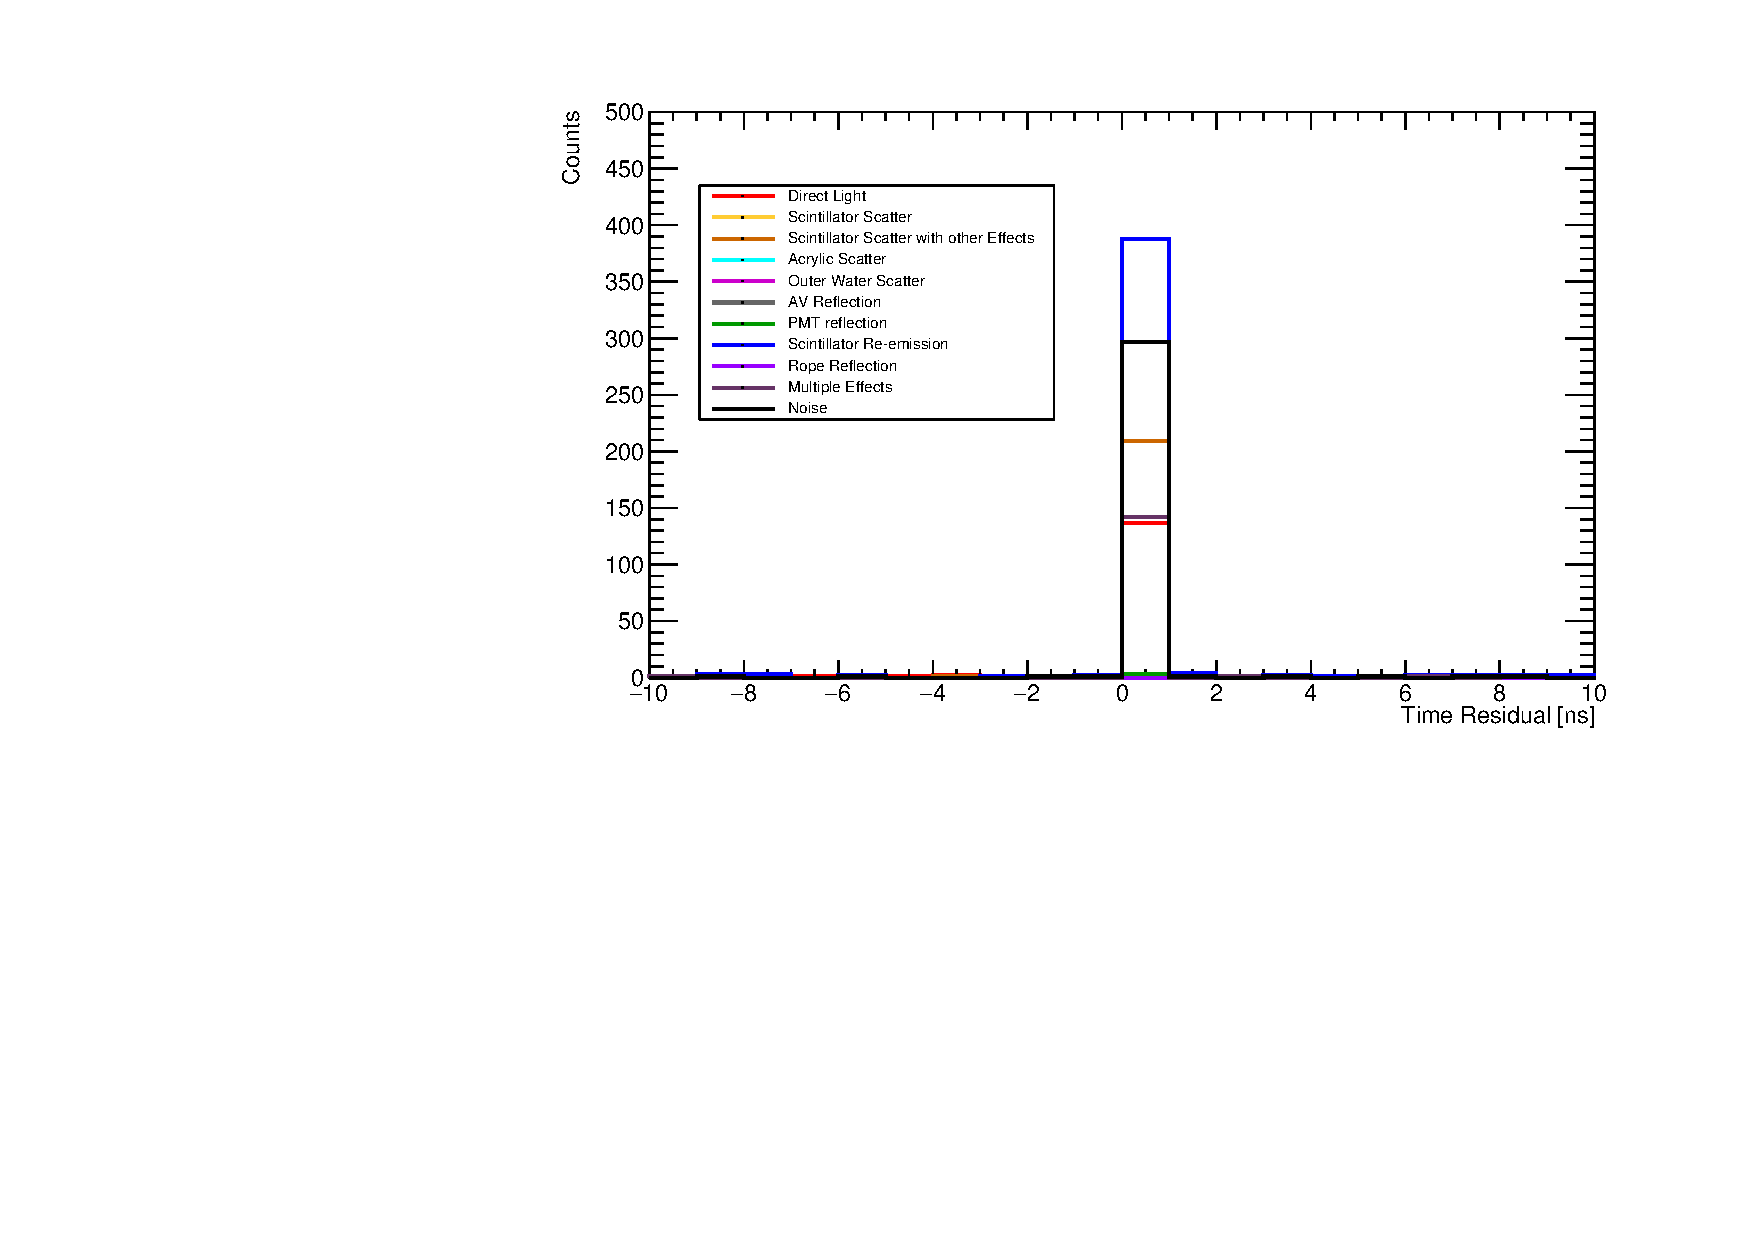
\includegraphics[width=0.8\textwidth]{5_SMELLIEAnalysis/images/far_pmts_tres_plot_FS007_PQ375.pdf}
    \caption[Unstacked time residual distribution of a simulation of light from the PQ375 laser firing through fibre FS007, split by optical components]
    {Unstacked time residual distribution of a simulation of light from the PQ375 laser firing through fibre FS007, split by optical components. The direct light is clearly subdominant to light that has been absorbed and re-emitted by the scintillator. The spike at \SI{0}{\ns} arises from only one hit being observed in the beamspot for that event.}
    \label{fig:smellie_PQ375_far_pmts_components}
\end{figure}

Although re-emitted light is sub-dominant in the far region, scattered light remains an important background. This becomes most relevant for the \ang{10} and \ang{20} fibres, as the direction of the far PMTs are somewhat distant from the beamspot, so the intensity of direct light is substantially less than that of the \ang{0} fibres. A simulation of this is shown in Fig.~\ref{fig:smellie_PQ407_FS107_far_pmts_components} for fibre FS107 in the \SI{2.2}{\gpl} scintillator phase. The proportion of direct light signal to background components in the $[-5,+5]\,\si{\ns}$ window is substantial. As a result, any measurement of $R_{s}$ would be systematically off. % have to introduce R_s, R_w notation earlier.

With similar simulations for all other fibres, it was found that all \ang{0} fibres apart from FS093 achieved a signal-to-background ratio of over 95\%. No other fibres were able to achieve a signal purity close to this value. Because of this, only these `pure' fibres were used for actual extinction length calculations in this analysis. Data from the other fibres was still processed, but only used for comparison, as will be seen in the next section. Unlike all other fibres, FS093 was found to have a strong contribution to the far PMT hits from light reflected off of ropes. Although this rope reflection contribution should not be impacted by changes to the inner detector medium, it was decided to leave this fibre out of the extinction length calculations.

\begin{figure}
    \centering
    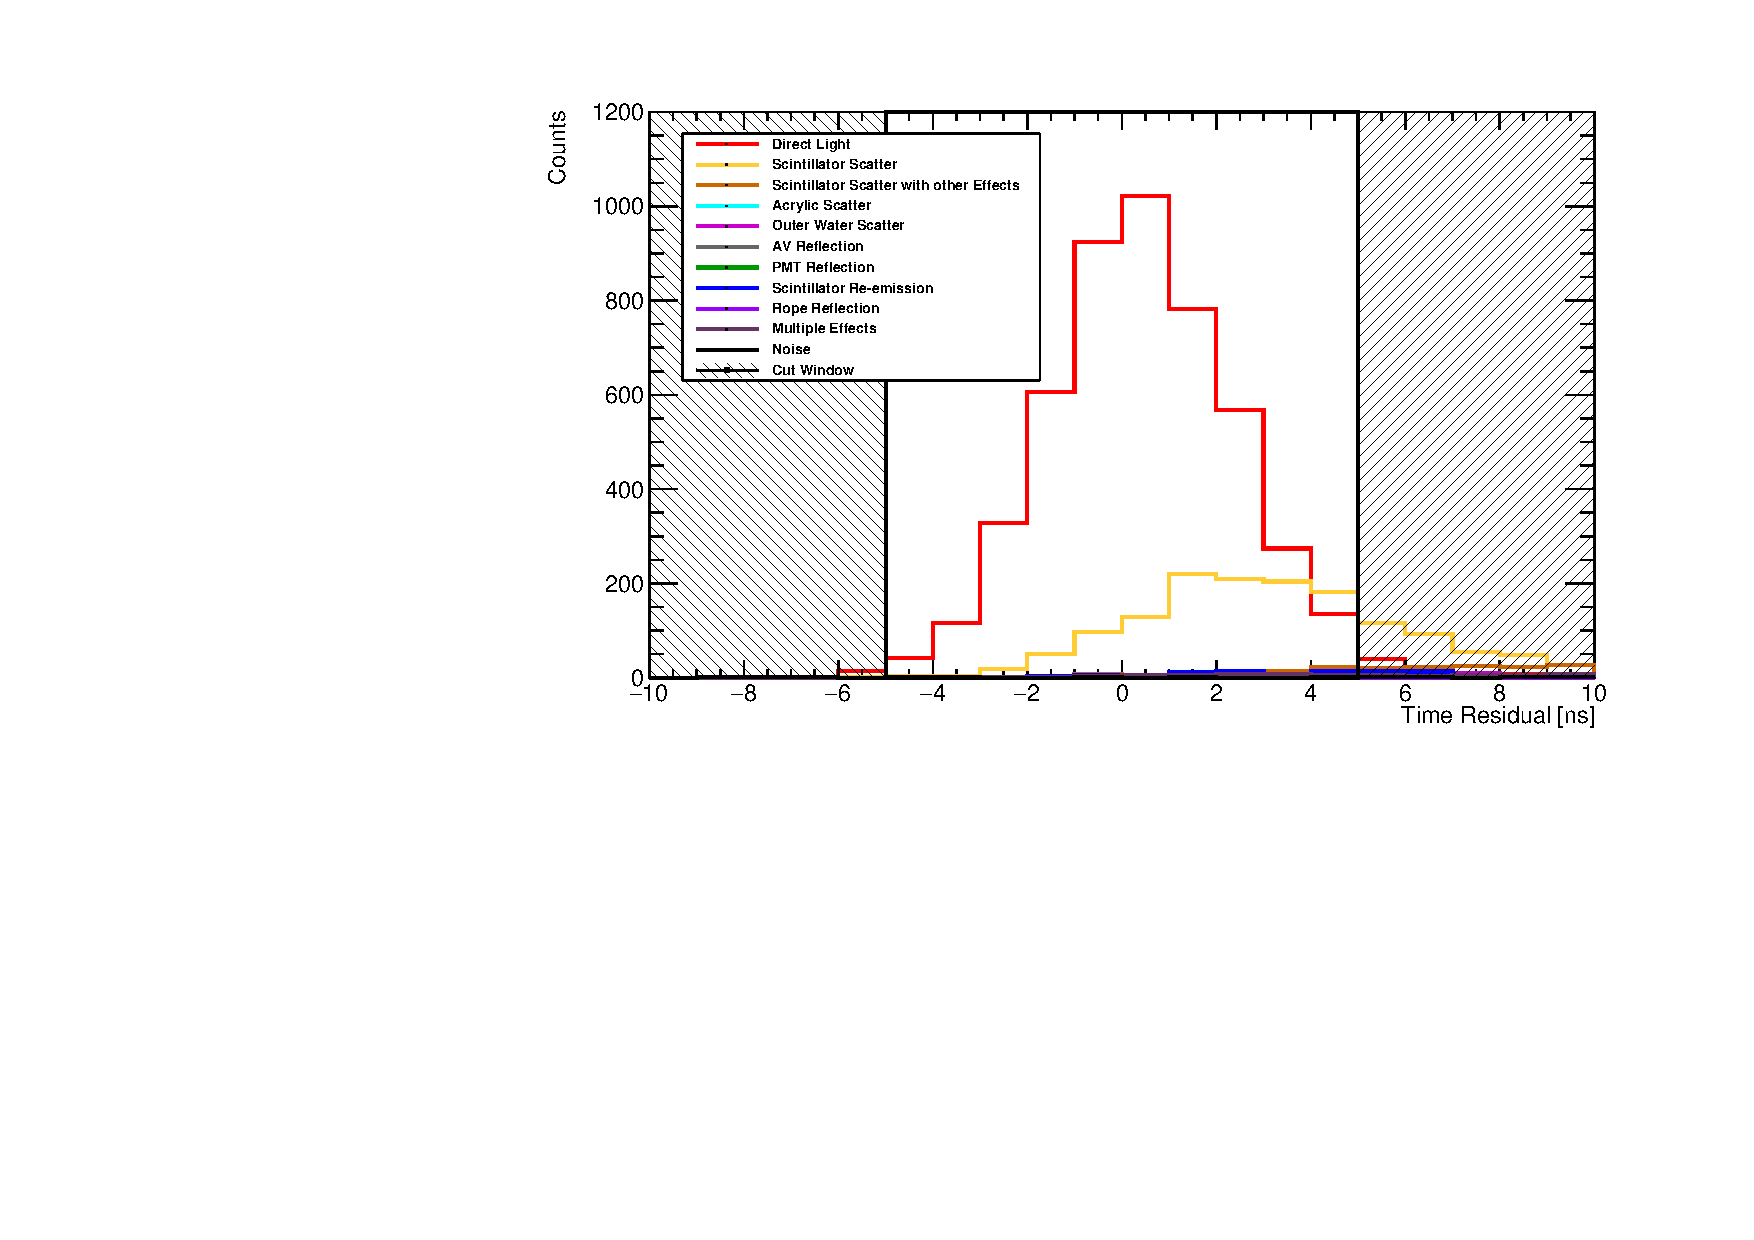
\includegraphics[width=\textwidth]{5_SMELLIEAnalysis/images/far_pmts_tres_components_nice_PQ407_FS107.pdf}
    \caption[]
    {Far PMT time window selection applied to a simulation of the PQ407 laser fired through laser FS107. The substantial background contribution from scattered light can be seen.}
    \label{fig:smellie_PQ407_FS107_far_pmts_components}
\end{figure}

\subsubsection{Results}\label{sec:smellie_ext_length_results}
The analysis results from the PQ407 laser are shown in Fig.~\ref{fig:smellie_ext_length_results_PQ407}. These have been split into a different plot for each time period. Each fibre is represented by an individual colour and marker shape pairing associated with the fibre's pointing angle and node, respectively. Because \ang{0} fibres had the far PMT region nearest the beamspot, they observed the largest values of $R_{w}$ and $R_{s}$ compared to the \ang{10} and \ang{20} fibres. This necessitated the use of log-log plots to effectively show the data. Lines of constant gradient, associated with scintillator extinction lengths in the range \SIrange{5}{120}{\m} in \SI{5}{\m} steps, are shown as dashed grey lines. These lines increase in extinction length from the top left down to the bottom right, and in so doing show that longer extinction lengths are much harder to measure with the same precision as shorter extinction lengths.

\begin{sidewaysfigure}
    \centering
    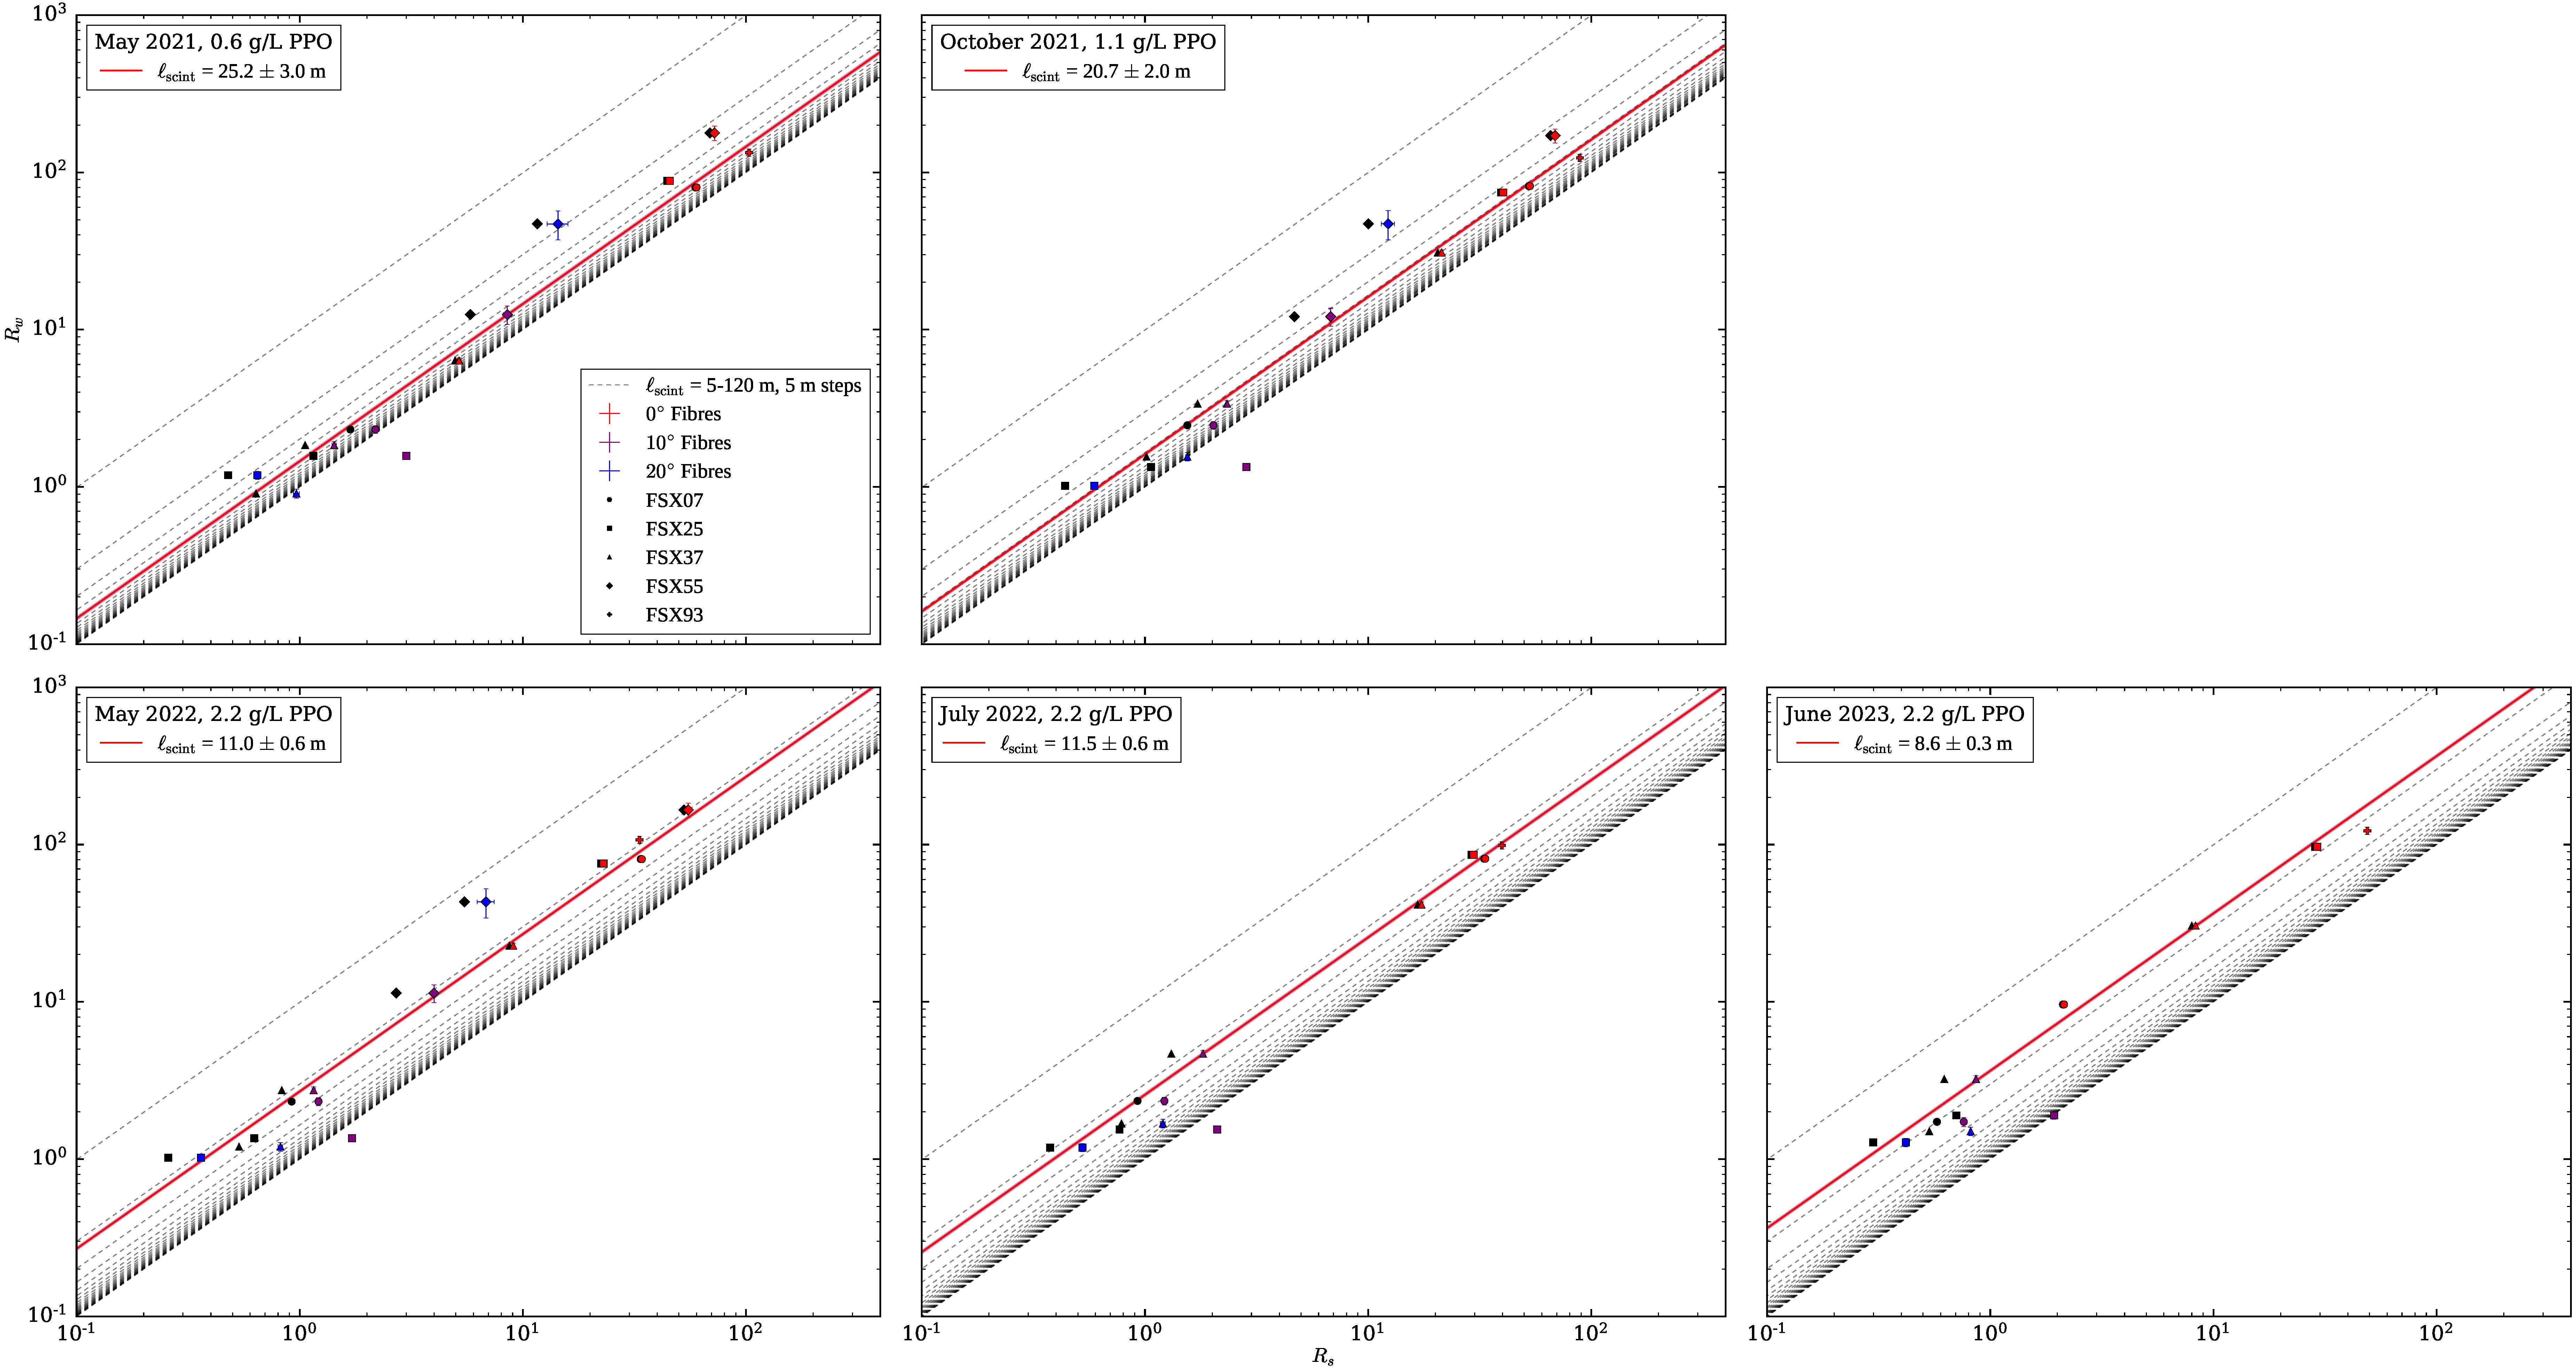
\includegraphics[width=\textwidth]{5_SMELLIEAnalysis/images/rsrw_plot_combined_PQ405.pdf}
    \caption[Results of the extinction length analysis using the PQ407 laser]
    {Results of the extinction length analysis using the PQ407 laser.}
    \label{fig:smellie_ext_length_results_PQ407}
\end{sidewaysfigure}

As explained in the previous section, each plot had a straight line of the form $R_{w} = mR_{s}$ fit to the \ang{0} data points, excluding fibre FS093. Because there were comparable uncertainties in both axes, this fit was performed by minimising the $\chi^{2}$ term:
\begin{equation}
    \chi^{2}(m) = \sum_{j}\frac{\left(R_{j,w} - mR_{j,s}\right)^{2}}{\sigma^{2}_{R_{j,w}} + m^{2}\sigma^{2}_{R_{j,s}}}.
\end{equation}
An uncertainty on the gradient of the fit was found by determining the change in $m$ required to increase the value of $\chi^{2}(m)$ by 1. Re-arranging Eq.~\ref{eq:smellie_ext_length_rsrw_formula_1PMT}, one can derive the formula:
\begin{equation}
    l_{\mathrm{scint}} = 
    \frac{
        L_{s}
        }{
        \ln{m}
        + \ln\left(
            \frac{T_{s}}{T_{w}}
        \right)
        + \frac{L_{w}}{l_{w}}
    },
\end{equation}
from which the extinction length in scintillator at a given wavelength at a given time period with propagated uncertainties was found.

As the concentration of PPO is increased in the detector, the extinction length at 407 nm appears to decrease in tandem. Then, the first two datasets taken in the \SI{2.2}{\gpl} scintillator phase appear consistent with one another. This is not true of the final dataset taken at the end of the scintillator phase, which measured a shorter extinction length again. The origin of this change is unknown.

Also shown in the plot are the results of fibres not included in the fit. As an example, fibre FS125 (shown as the purple square) is found to be generally in the non-physical region corresponding to negative extinction lengths, in the bottom-right half of the plots. This can be explained by the substantial scattering background expected in the far PMTs of this fibre. Assuming the simulation discussed in the previous section for this fibre in the \SI{2.2}{\gpl} scintillator phase, as well as matching simulations for the other PPO concentrations, this systematic effect in $R_{s}$ was corrected for and shown with a black square. This was also shown for all other fibres. As can be seen, by using the nominal correction from the existing scintillator optics models, the FS125 measurements are pushed into the physical regime, quite close to the line of best-fit.

\begin{sidewaysfigure}
    \centering
    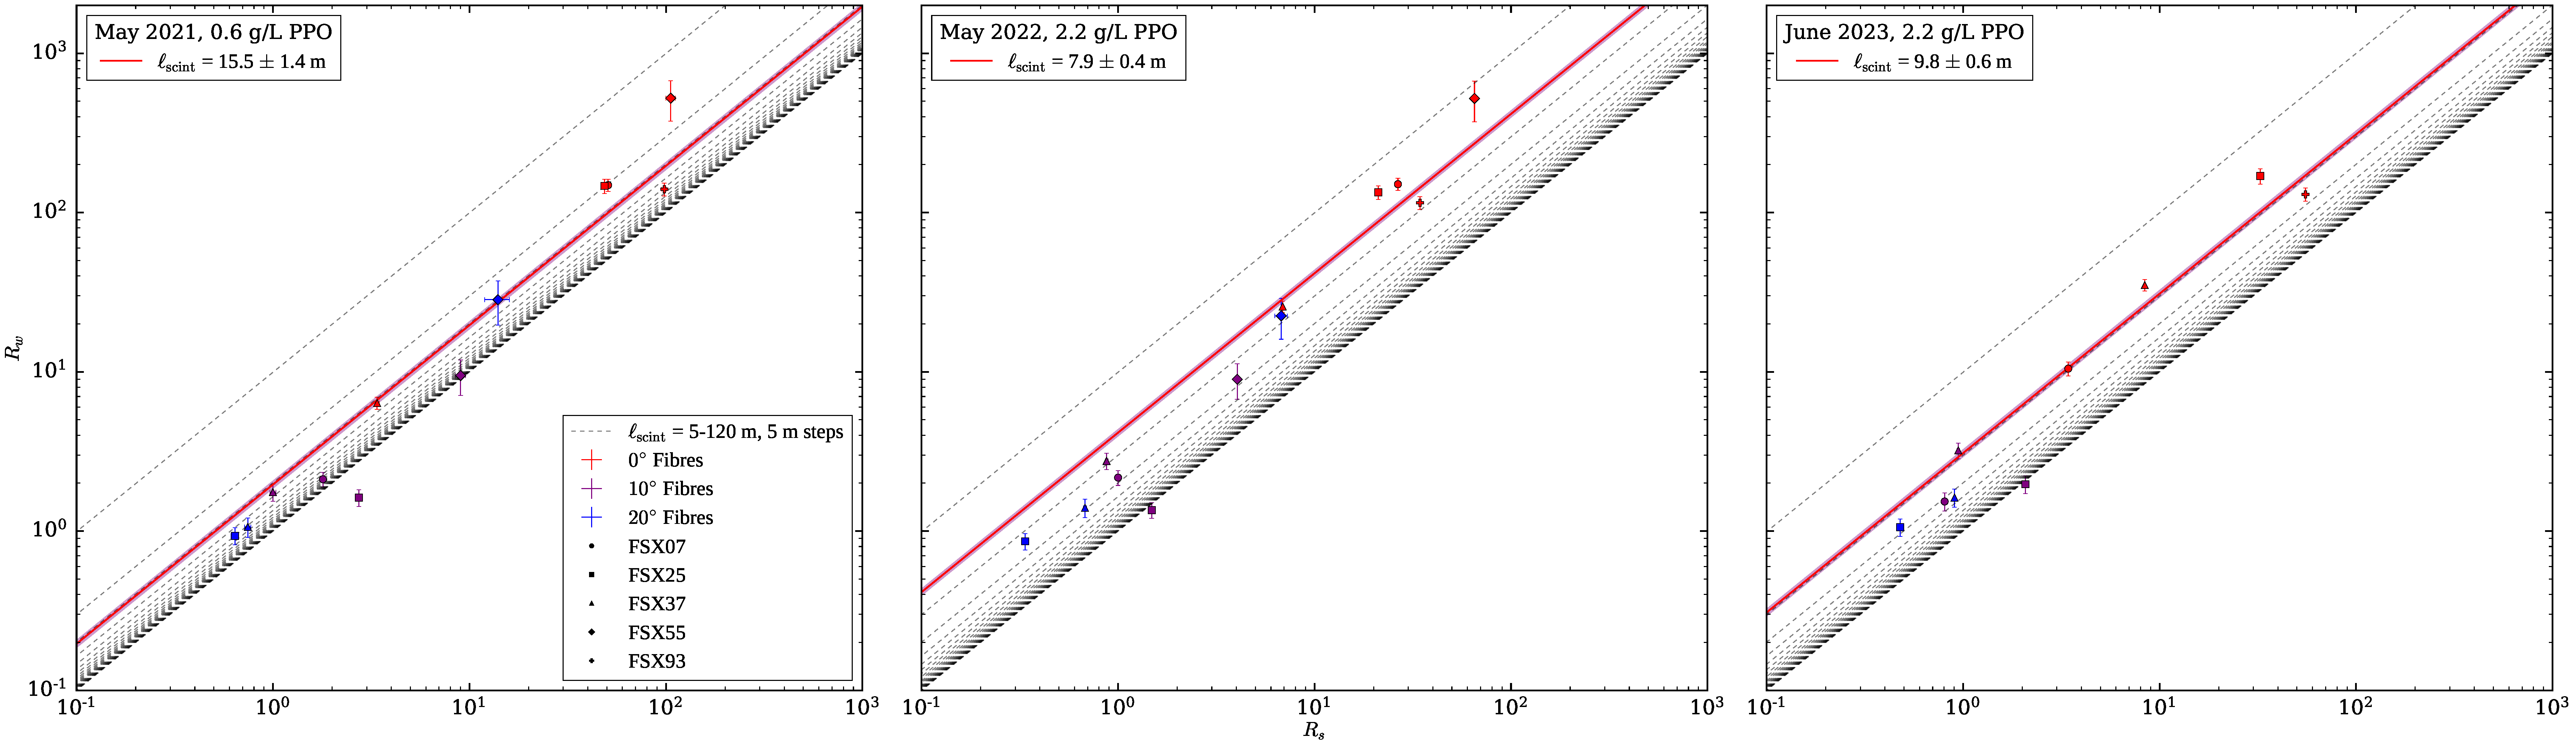
\includegraphics[width=\textwidth]{5_SMELLIEAnalysis/images/rsrw_plot_combined_superK[400,410].pdf}
    \caption[Results of the extinction length analysis using the SuperK laser in the \SIrange{400}{410}{\nm} range]
    {Results of the extinction length analysis using the SuperK laser in the \SIrange{400}{410}{\nm} range.}
    \label{fig:smellie_ext_length_results_SK_400410}
\end{sidewaysfigure}

Fig.~\ref{fig:smellie_ext_length_results_SK_400410} shows the data from the SuperK laser in the \SIrange{400}{410}{\nm} range, for the May 2021, May 2022, and June 2023 datasets in which SuperK data was taken. Once again, there appears to be a substantial shortening of the scintillator's extinction length as PPO was added. These values differ from the PQ407 result, but this is not too surprising as what is measured with the SuperK laser is the extinction length averaged over a whole \SI{10}{\nm} range, weighted by the intensity spectrum of the laser. The third measurement result increases compared to the second here, another contrast to the PQ407 laser.

% It is possible that the observed changes in these measurements between 2022 and 2023 are not a result of changes to the scintillator, but instead indirectly a result of the SMELLIE hardware changes made in the Summer of 2022 causing a systematic effect on the measurements. One possible way this could occur is through the instability of the laser intensities before the addition of the VFA. Fig.~\ref{fig:smellie_ext_length_far_pmt_tres_plot_comparison} shows the observed time residual distribution for far PMTs for fibre FS007 using laser PQ407 in the water phase data, as well as scintillator data of July 2022 and June 2023. The first two datasets show a clear spike of events at $\tres{} = 0$, corresponding to events with only one hit in the beamspot (and far PMT) region. This spike was substantial for these datasets, because of the substantial laser intensity instability discussed in Section~\ref{sec:smellie_attenuators}. However, the third dataset was taken after the installation of the VFA, meaning the laser intensities were stabilised event-by-event. This led to far fewer `spike' hits. This change in the shape of the time residual distribution leads to a change in the signal purity and efficiency within the `prompt' time window, causing a systematic shift.

% \begin{figure}
%     \centering
%     % 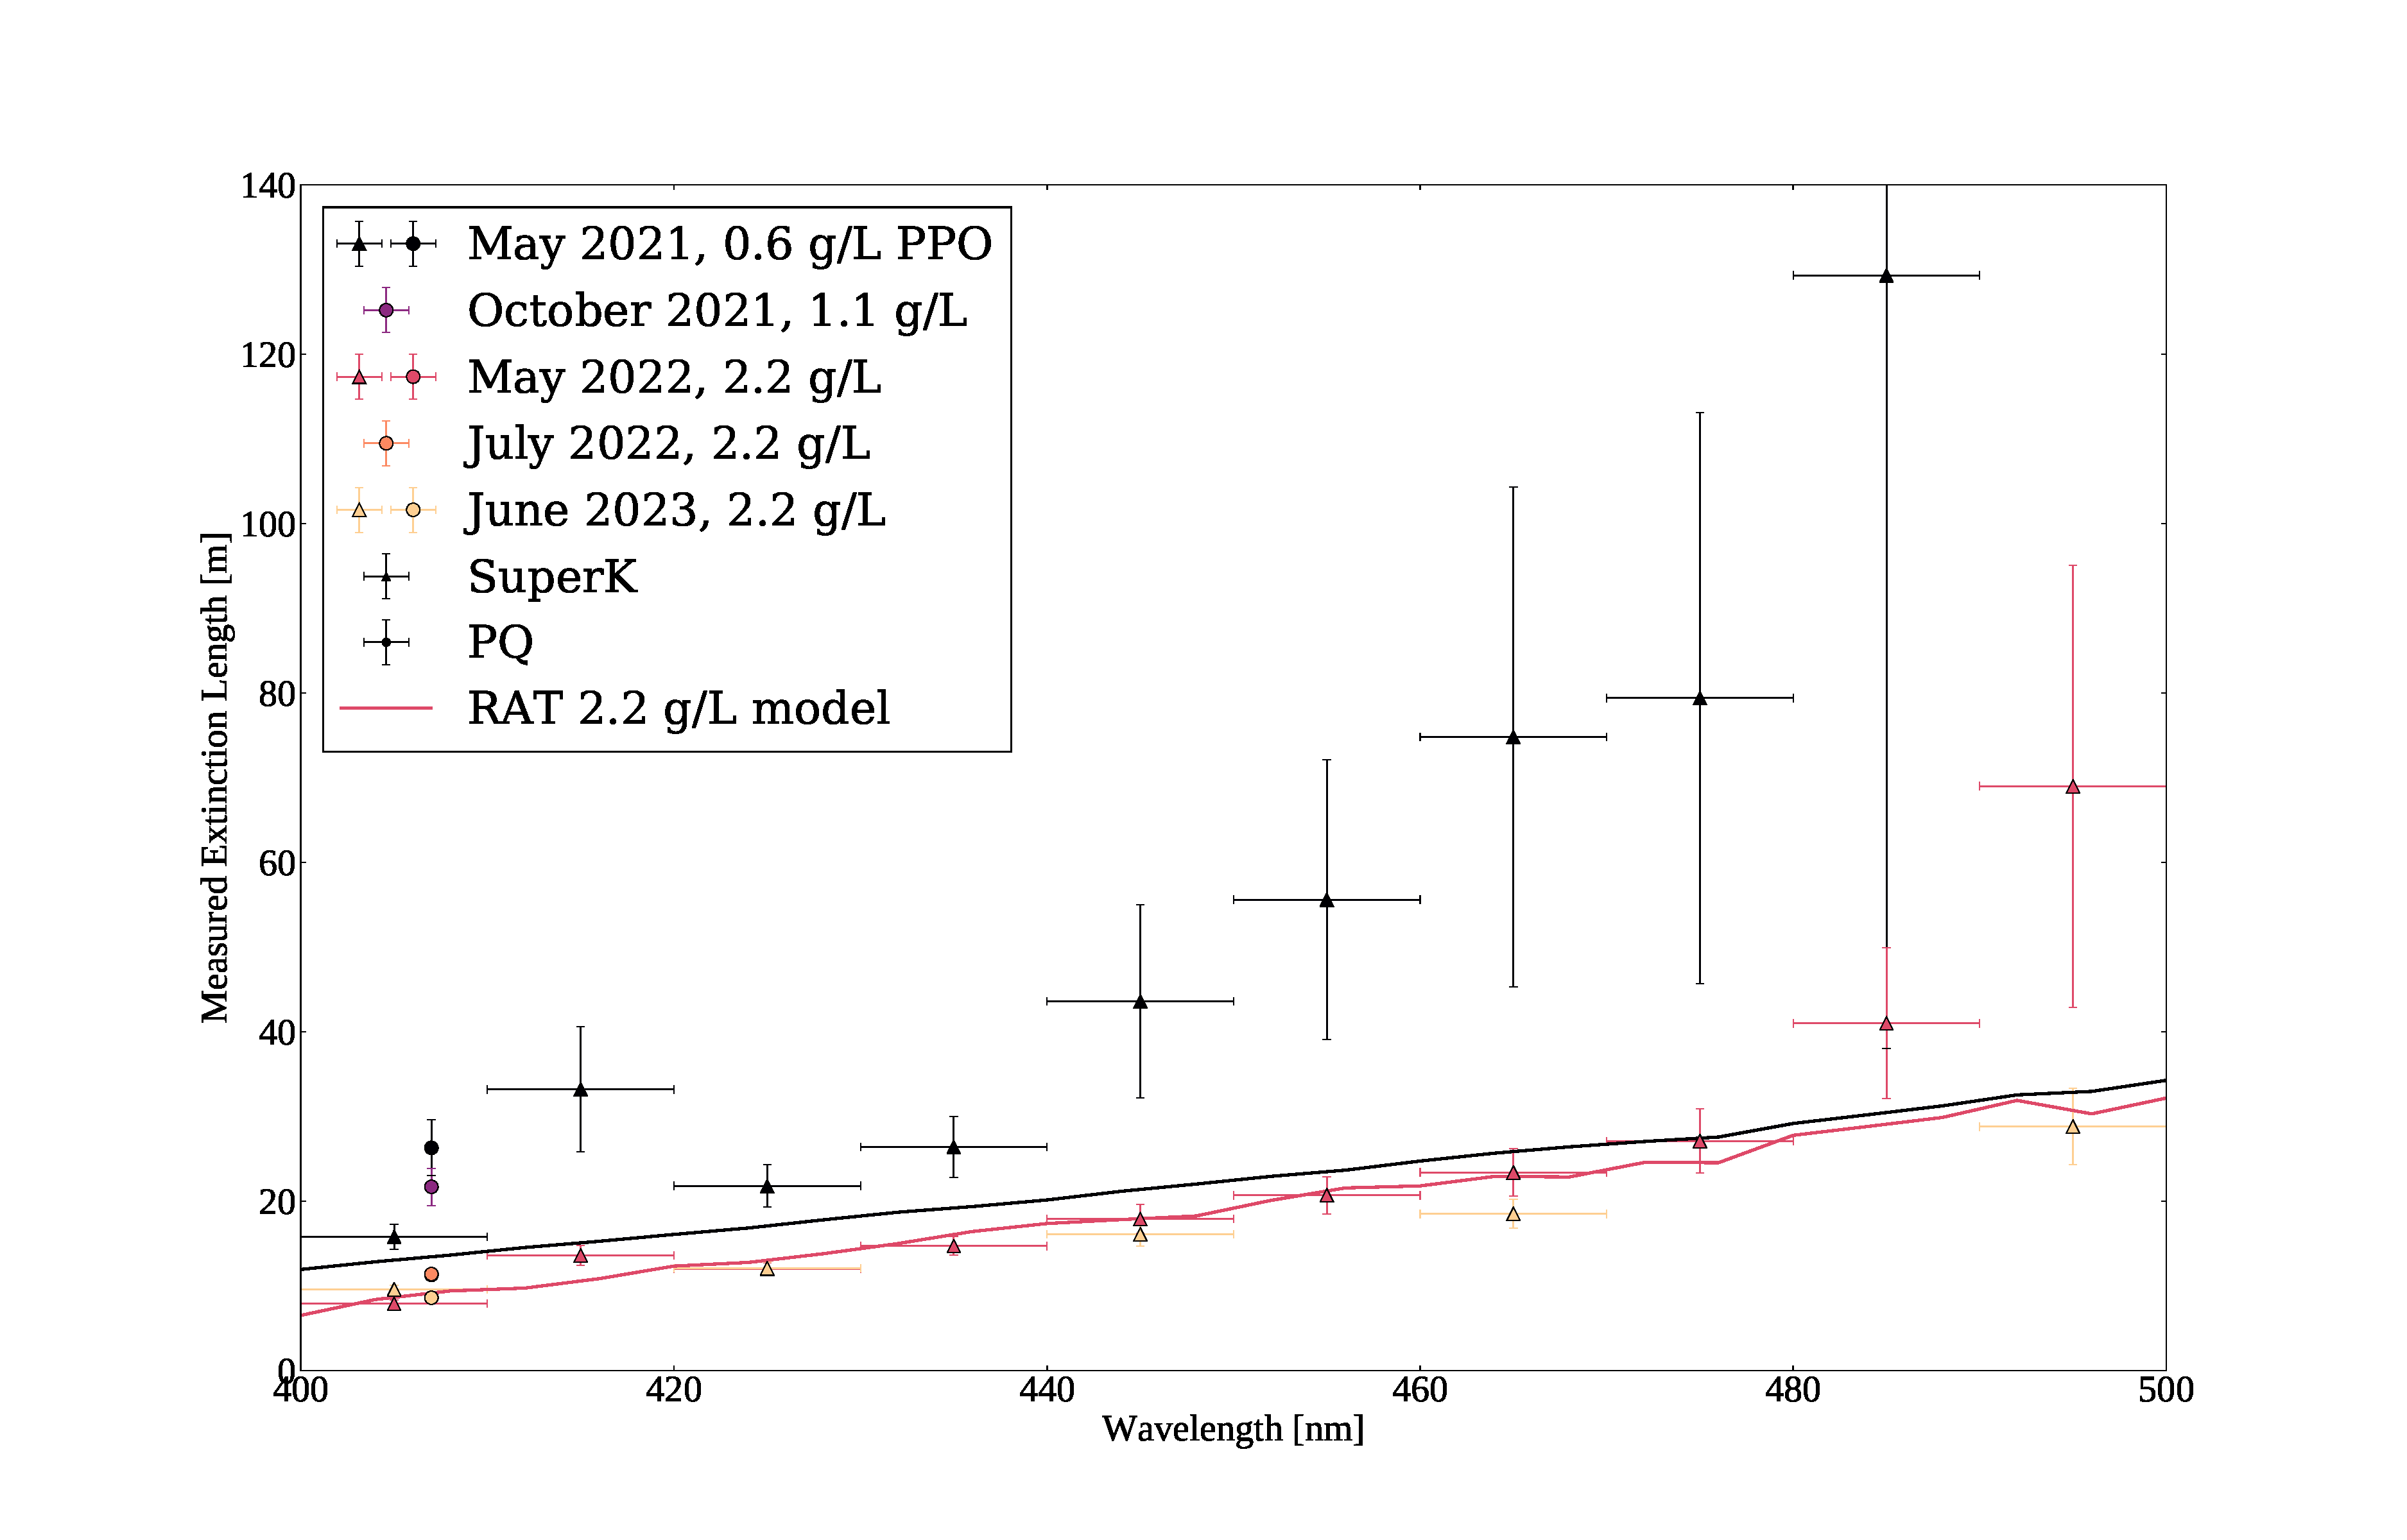
\includegraphics[width=\textwidth]{5_SMELLIEAnalysis/images/ext_length_results_summary.pdf}
%     \caption[]{}
%     \label{fig:smellie_ext_length_far_pmt_tres_plot_comparison}
% \end{figure}

Fits to the SuperK data at wavelengths between \SIrange{400}{500}{\nm} during May 2021, May 2022, and June 2023 were performed in the same manner as described above. The combined results for all of these measurements, as well as the PQ407 laser, are shown in Fig.~\ref{fig:smellie_ext_length_final_results}. All three SuperK datasets show an increase in the extinction length with wavelength, as expected. There is also a substantial shortening in the extinction length going from the \SI{0.6}{\gpl} dataset to the \SI{2.2}{\gpl} dataset. This is matched qualitatively with the PQ data. Generally, data from May 2022 and June 2023 appear to be consistent with one another.

\begin{figure}
    \centering
    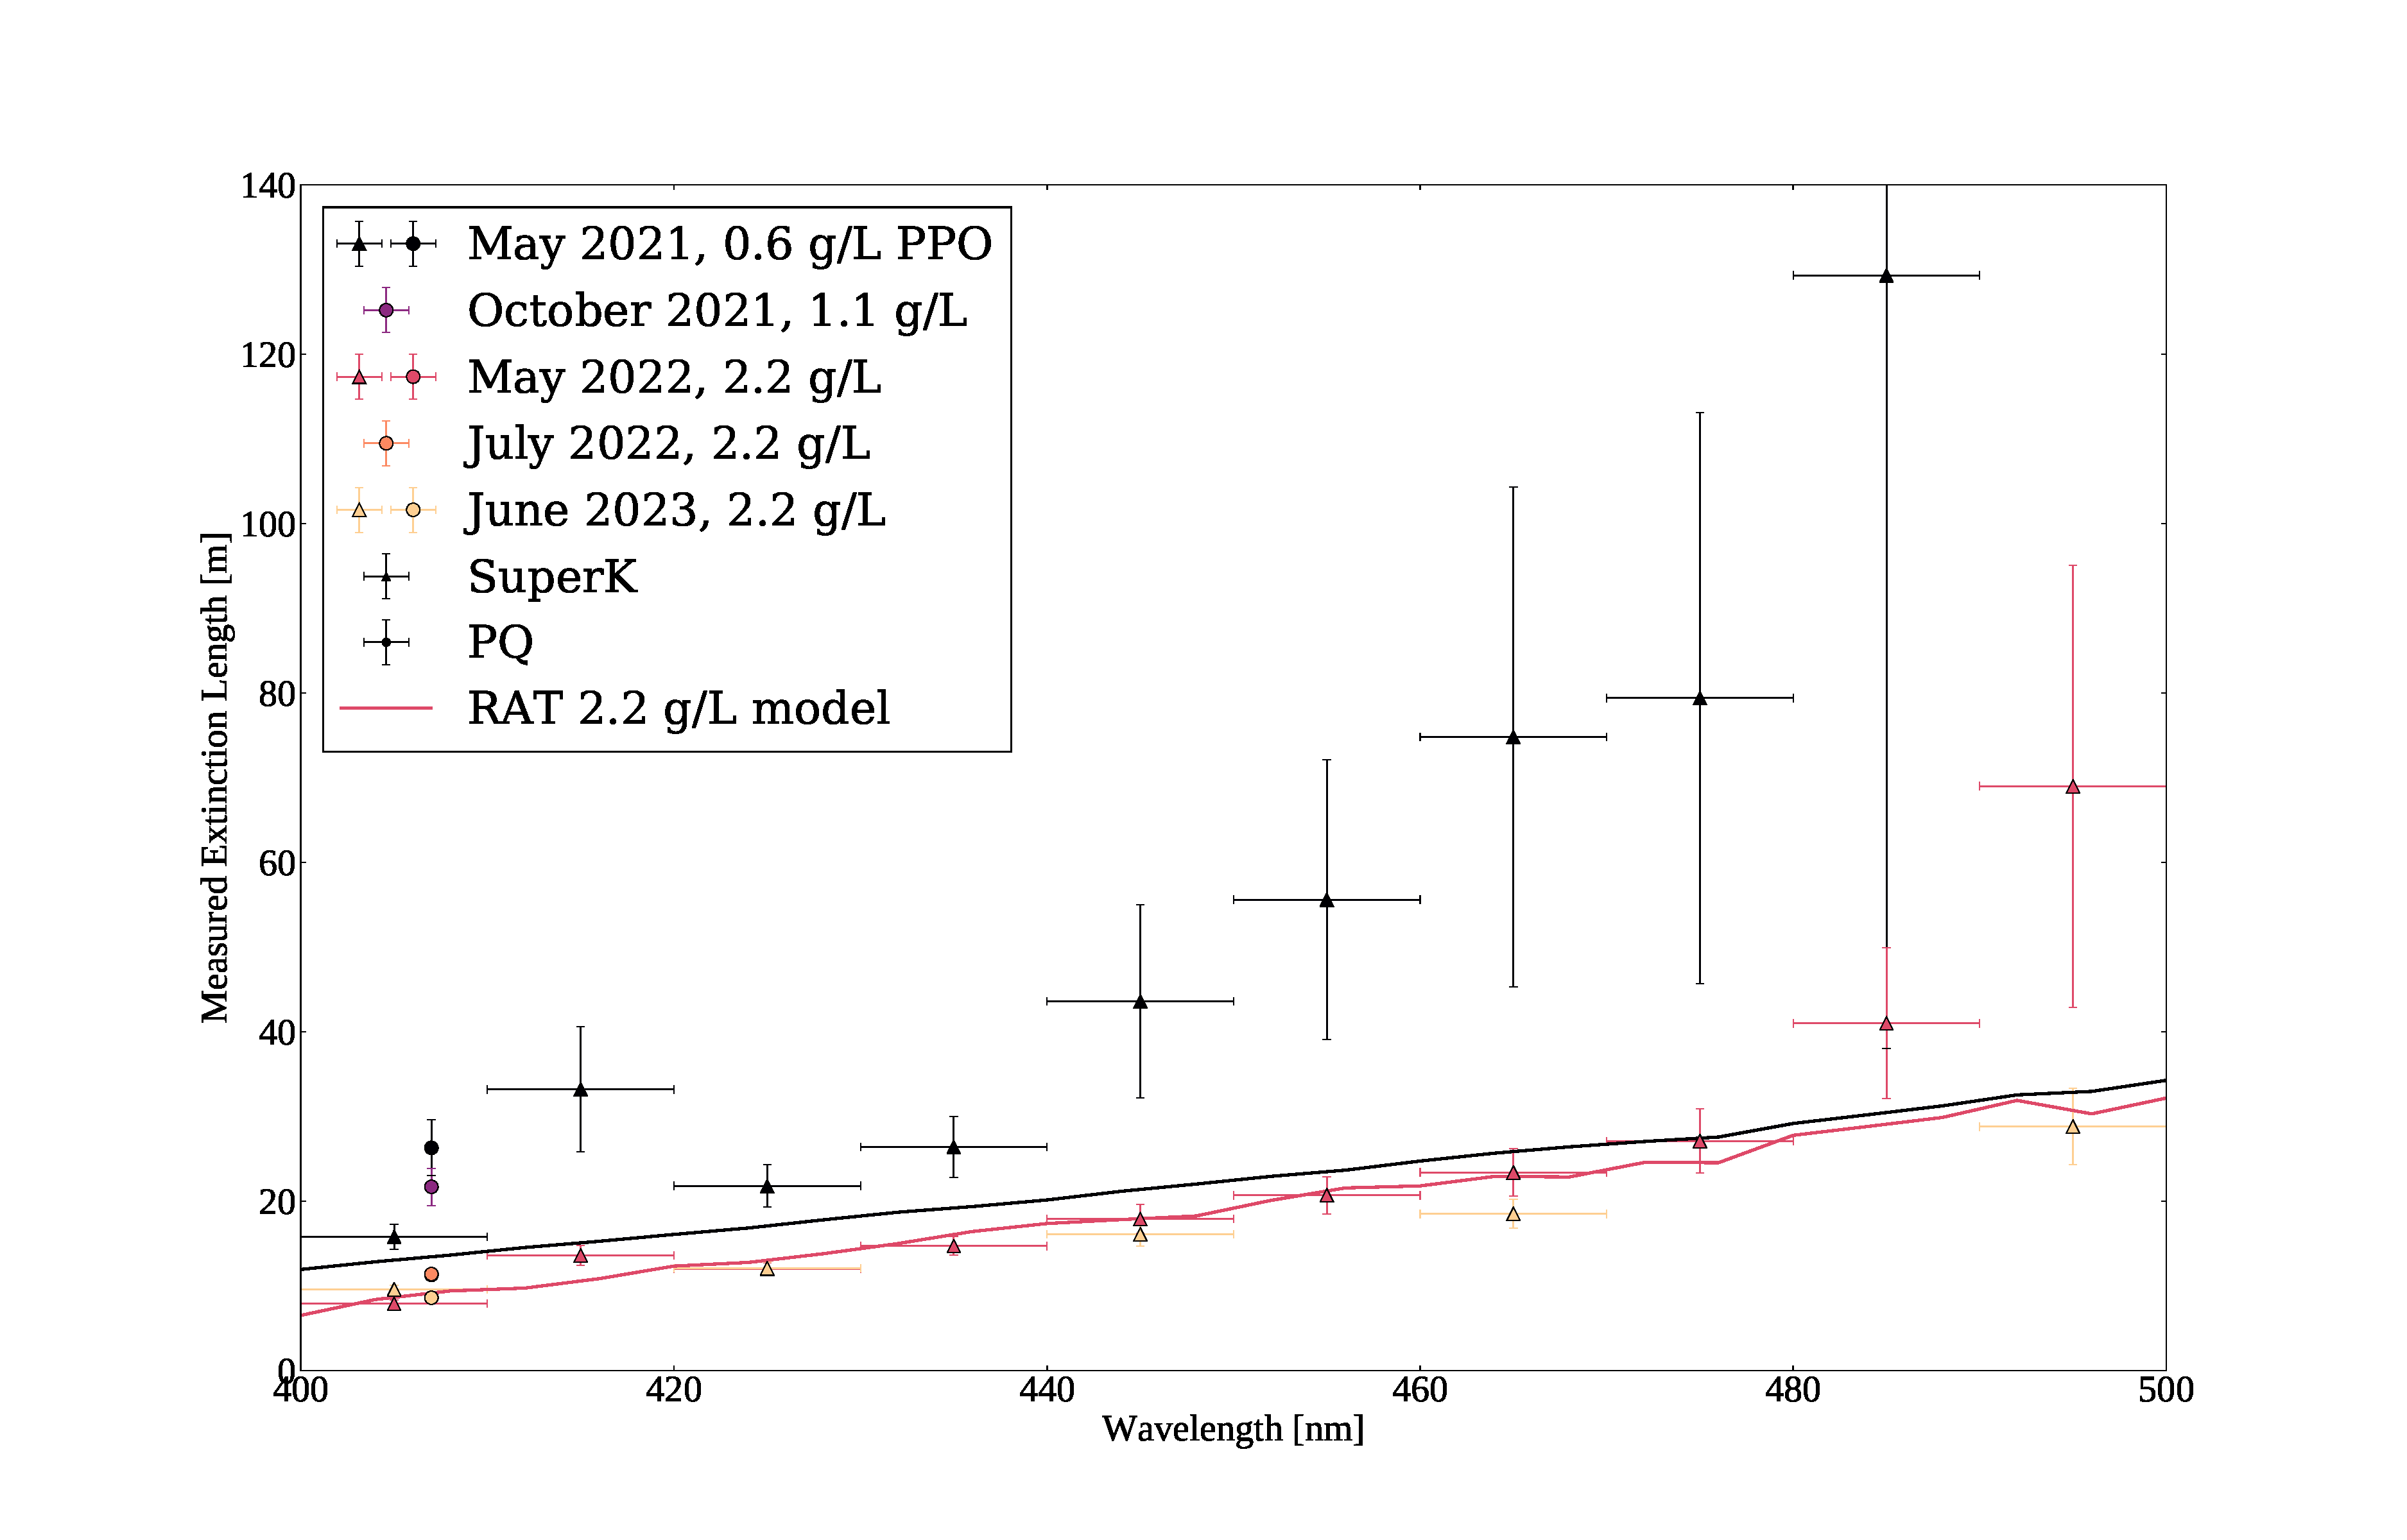
\includegraphics[width=\textwidth]{5_SMELLIEAnalysis/images/ext_length_results_summary.pdf}
    \caption[Summary of scintillator extinction length measurements made by SMELLIE]
    {Summary of scintillator extinction length measurements made by SMELLIE, with a comparison to the current \SI{2.2}{\gpl} optics model used in \texttt{RAT}.}
    \label{fig:smellie_ext_length_final_results}
\end{figure}

\subsubsection{Comparisons with other Measurements}\label{sec:smellie_ext_length_comparison}
It is important to compare the measurements of the scintillator extinction lengths using SMELLIE to other methods used by the Collaboration. The optical model used in \texttt{RAT} for the \SI{0.6}{\gpl} scintillator was built from bench-top measurements prior to scintillator phase~\cite{seguiScintillatorModelComparison2015,kaptanogluOpticsOverviewProposed2016}. The extinction length associated with this model is shown as a black line in Fig.~\ref{fig:smellie_ext_length_final_results}. The results from my analysis with SMELLIE data give longer extinction lengths than the existing model, for both the PQ and SuperK laser over all wavelengths in the \SIrange{400}{500}{\nm} region.

For the \SI{2.2}{\gpl} scintillator, more techniques were used for measurement of the extinction length. One approach by Ben Tam was to use `UV-vis' spectroscopy on samples of the scintillator extracted from the detector~\cite{tamBenchtopAttenuationMeasurements2022}. % cite Ben's thesis, DocDB?
Another method, used by Serena Riccetto, was to look at the \texttt{nhits} distribution of the radioactive background \ce{^{210}Po} within the detector: a discussion of this and other backgrounds in the detector can be found in Section~\ref{sec:background_processes}. The peak \texttt{nhit} value associated with this background varies with the position of the event, because of the changing lengths of scintillator the event's scintillation light must travel through. Different optical models could then be tested by comparing the peak \texttt{nhits} of the \ce{^{210}Po} in simulation to data~\cite{riccettoFullFill2102022}. % cite Serena's work.

The current model of the \SI{2.2}{\gpl} scintillator absorption and scattering used in \texttt{RAT} was developed by combining the measurements of B. Tam and S. Riccetto with older bench-top measurements made before the scintillator phase: details about this model-building can be found in~\cite{kaptanogluDocumentationAttenuationStudies2022,riccettoRATOptics2g2022}. % cite Serena's explanation; older measurements.
The extinction lengths obtained from this model are shown as a red line in Fig.~\ref{fig:smellie_ext_length_final_results}. There appears to be good agreement between these model values and the results from the analysis with SMELLIE data taken in May 2022 for wavelengths in the ranges \SIrange{400}{430}{\nm} and \SIrange{490}{500}{\nm}. At medium wavelengths, SMELLIE appears to measure extinction lengths somewhat shorter than the existing \texttt{RAT} model. These results appear consistent between the May 2022 and June 2023 datasets.


% \begin{itemize}
%     \item Describe the data used in this analysis, both water and scintillator, which can be shown in a table.
%     \item Show examples of analysis of data in action for \SI{375}{\nm} data: typical $t_{\textrm{res}}$ distributions of backscattered and beamspot PMTs; calculation of that particular extinction length measurement, followed by the graph for extinction length in \SI{375}{\nm} over all fibres and time periods.
%     \item Discuss what results can be seen in this plot: consistency between fibres, the expected change as a function of PPO concentration, and stability of the extinction length during the main \SI{2.2}{\gpl} scintillator phase.
%     \item Compare results to those made by Ben ex-situ: are they in agreement? If not, what possible systematics could there be? The main one for my analysis is likely to be uncertainties in the simulated beam profile that leak through into the refractive index correction of the beamspot. For the ex-situ analysis, the value of the extinction length obtained is achieved through background subtraction at some long wavelength, and the particular choice of this wavelength can lead to systematic changes in the obtained extinction length.
%     \item Look at results at longer wavelengths: can anything reasonably be said at these longer wavelengths? Why/why not?
%     \item Finally: describe any conclusions that can be reached, in particular whether we can affirm the optics model we use in RAT.
% \end{itemize}
% [8 pages]


\section{Scattering Analysis}\label{sec:scattering_analysis}
\subsection{Historical Approaches and the Problem of Systematics}
A method for measuring scattering lengths in the detector using SMELLIE was first developed by K. Majumdar~\cite{majumdarMeasurementOpticalScattering2015}. This method was used by E. Turner to measure the scattering length of the UPW in the water phase~\cite{turnerMeasurementScatteringCharacteristics2022}. A similar approach was built by S. Langrock, and tested on fake water phase data~\cite{langrockMeasurementRayleighScattering2016}. The general analysis technique was as follows:
\begin{enumerate}
    \item Using simulations under nominal conditions, a region of PMTs and associated time windows was selected that optimised the sensitivity to hits from photons that were scattered inside the AV. This signal region was defined by a geometric region of the 2D $(\tres{},\alpha)$ parameter space.
    \item Data was taken using the SMELLIE system.
    \item A calibration curve of the fraction of hits in the scattered signal region to that of the whole detector as a function of the scattering length for a given fibre and wavelength, was built using simulations.
    \item The fraction of hits in the signal region was determined for each subrun of SMELLIE data, and then the calibration curve was used to derive values of the scattering length at that wavelength.
\end{enumerate}

The challenge with this analysis approach is that it relies on the use of SMELLIE simulations to derive results. There are substantial systematic uncertainties in the modelling of the SMELLIE beam profiles, which can readily propagate into the uncertainty of the scattering length measurement. Both S. Langrock and E. Turner found this in their analyses~\cite{langrockMeasurementRayleighScattering2016,turnerMeasurementScatteringCharacteristics2022}. Furthermore, the signal regions chosen historically had a substantial background contribution, which often appeared to not be modelled with sufficient accuracy.

As a demonstration of these problems, consider a comparison between PQ495 laser data taken in July 2022, through fibre FS055, to a simulation of the same setup. This is shown in Fig.~\ref{fig:smellie_tres_alpha_data_mc}. Also shown in these plots is the scattering signal region as determined by K. Majumdar and E. Turner's method. One can observe qualitatively features that differ between the data and MC. % DETAILS?
Furthermore, Fig.~\ref{fig:smellie_tresalpha_mc2} shows the impact of using a modified beam profile in the simulation. Instead of using the beam profile developed for that fibre in Section~\ref{sec:combining_beam_profiles}, one was used that had data from only one water phase subrun, as shown in Section~\ref{sect:new_gen}. The fraction of hits in the signal region changes from 31.2\% to 27.7\%.

\begin{figure}
    \centering
    \begin{subfigure}{0.98\textwidth}
        \centering
        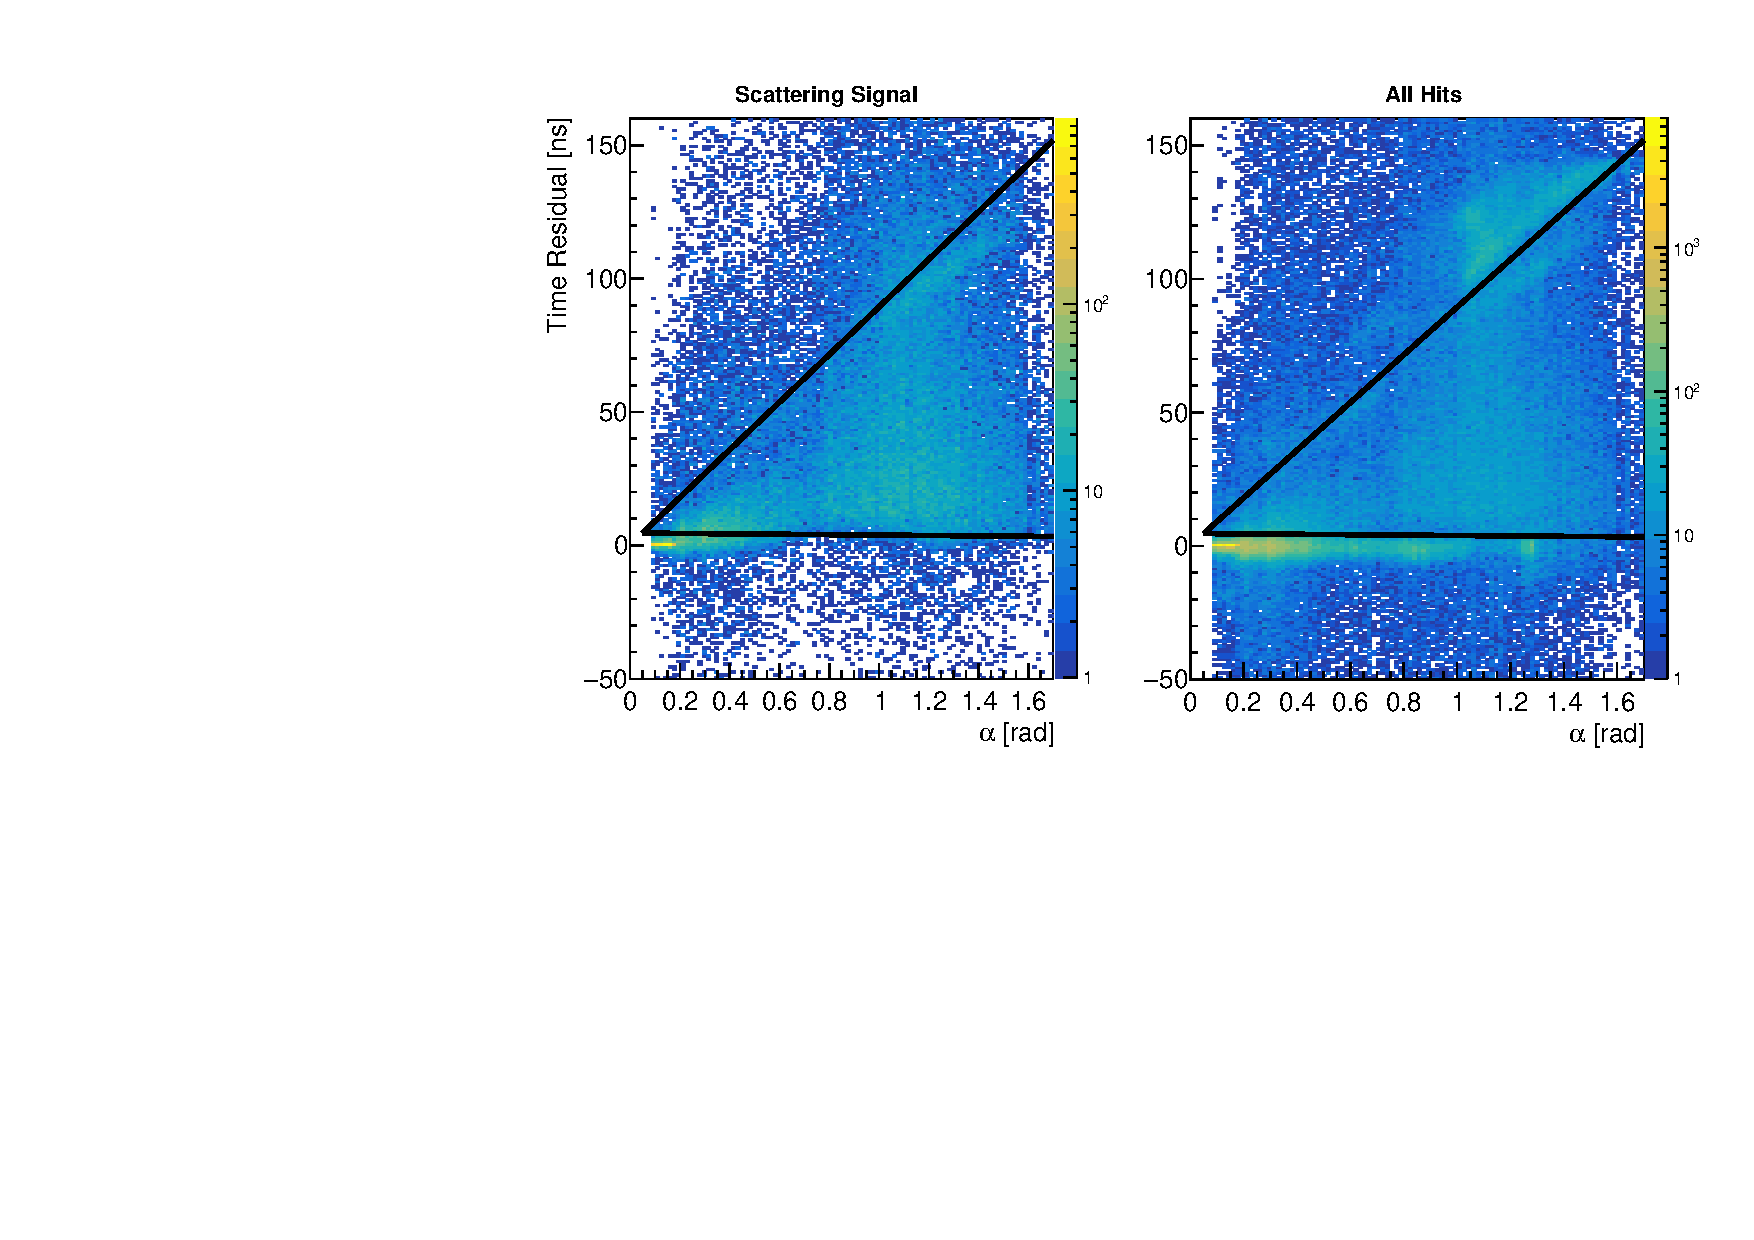
\includegraphics[width=\textwidth]{5_SMELLIEAnalysis/images/FS055_PQ495_new_beam_profile_signal_vs_all_tres_alpha_plot.pdf}
        \caption{New beam profile}
        \label{fig:smellie_tresalpha_mc}
    \end{subfigure}
    \begin{subfigure}{0.98\textwidth}
        \centering
        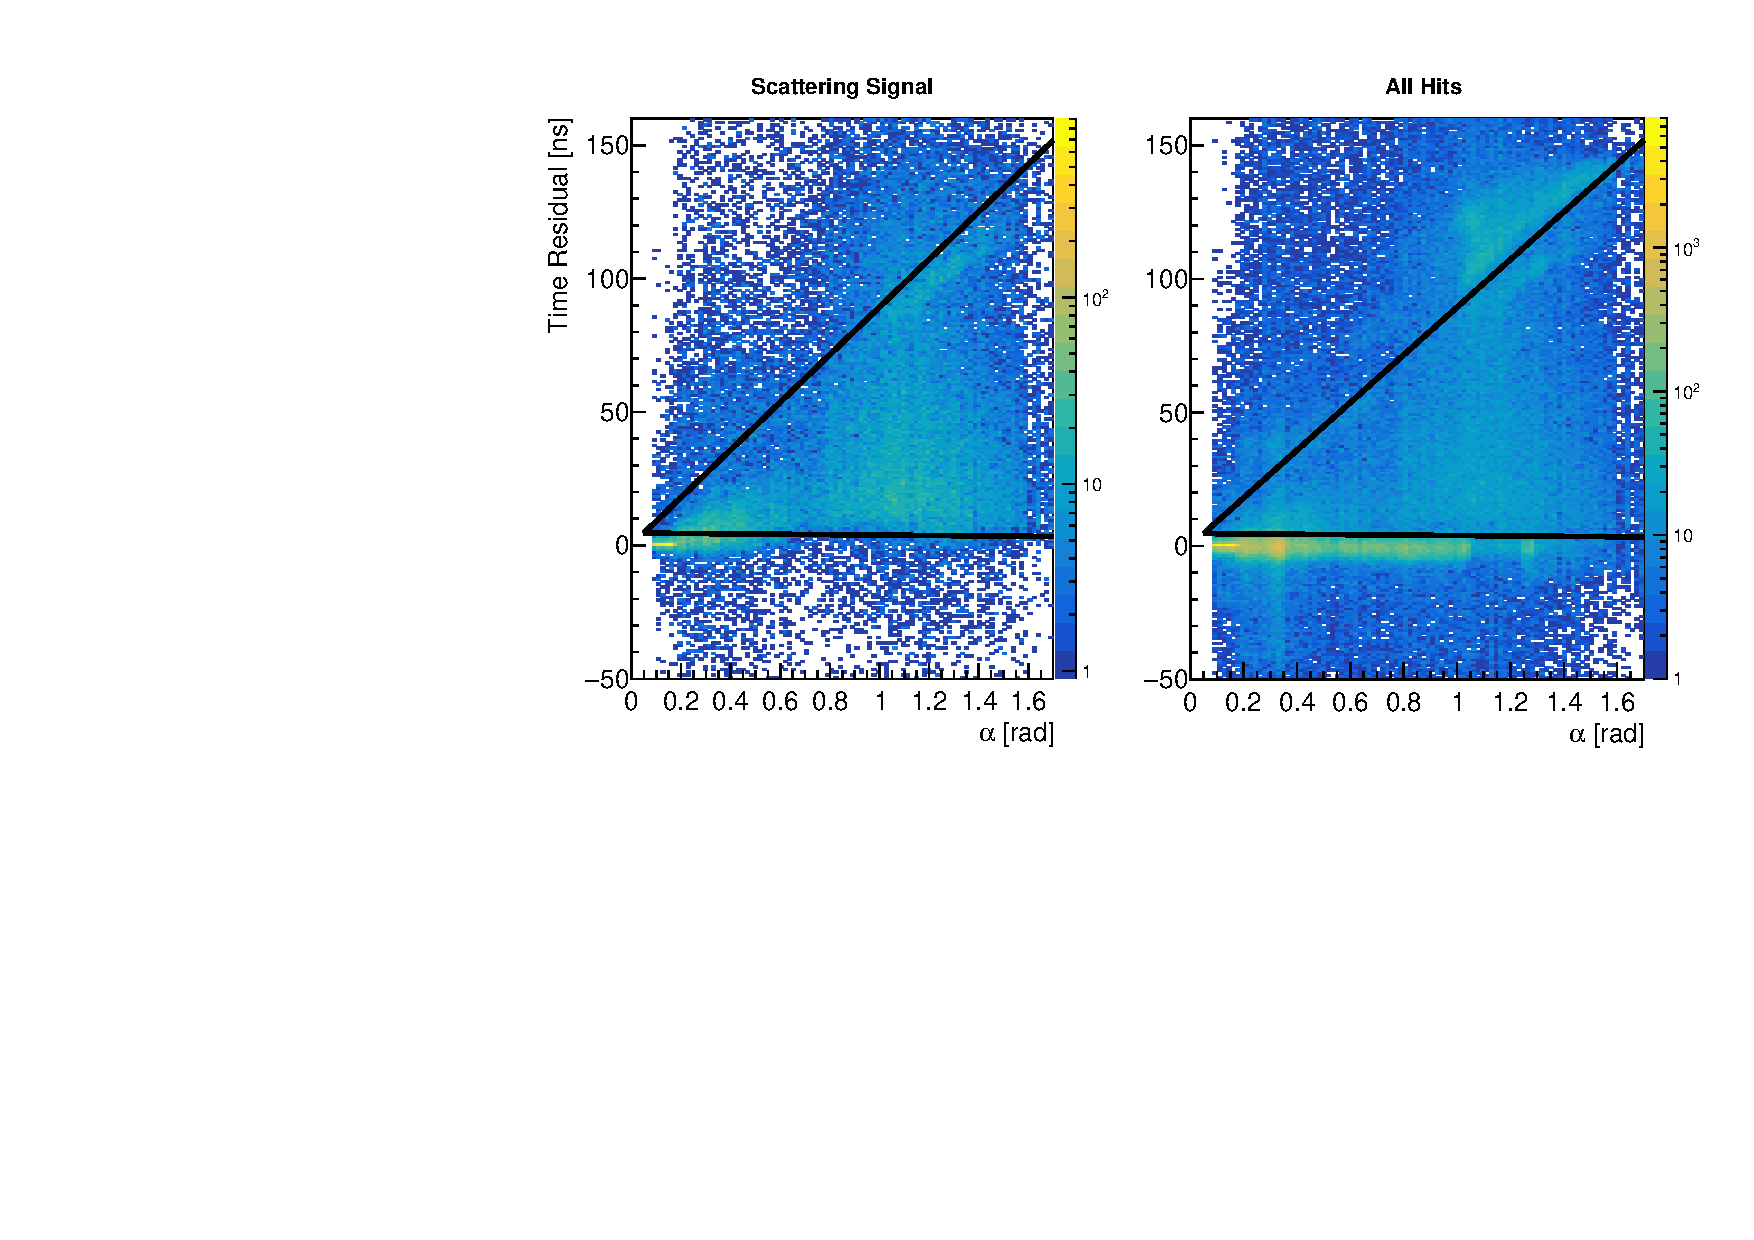
\includegraphics[width=\textwidth]{5_SMELLIEAnalysis/images/FS055_PQ495_old_beam_profile_signal_vs_all_tres_alpha_plot.pdf}
        \caption{Old beam profile}
        \label{fig:smellie_tresalpha_mc2}
    \end{subfigure}
    \caption[Comparison of the signal and total hit distribution in the $(\tres{},\alpha)$-space using new and old beam profiles for laser PQ495 through fibre FS055]
    {Comparison of the signal and total hit distribution in the $(\tres{},\alpha)$-space using new and old beam profiles for laser PQ495 through fibre FS055. The triangular scattering signal region of K. Majumdar's analysis are shown, optimised for the new beam profile simulation. The fraction of all hits in this signal is 31.2\% for the new beam profile simulation, and 27.7\% for the old beam profile.}
    \label{fig:smellie_tres_alpha_data_mc}
\end{figure}

There are two major approaches to handling the problems described above. One approach is to build an optical model of the detector and SMELLIE that has negligible systematic uncertainties, so that the existing analysis approach can be used with minimal problems. An alternative approach, and the one used in this thesis, is to build a new analysis that is more robust to the existing systematic uncertainties in both the SMELLIE beam profile and detector optics.


% \begin{itemize}
%     \item Comparison to MC is necessary in scattering analysis, compared to merely being needed as a correction factor. This is because of the angular dependence of scattering. As a result, we can be far more susceptible to systematics from poor modelling!
%     \item As a warning, show how Krish's/Esther's approach to the SMELLIE scattering analysis suffers majorly from these systematic effects. Requires describing their analysis approach briefly, and then explaining how the systematics described in Section~\ref{sec:smellie_systematics} lead to major problems with this approach.
%     \item Motivates the need for either reduced systematics, or an alternative analysis approach that is more robust to them!
% \end{itemize}
% [2 pages]
\subsection{New Methodology}\label{sec:smellie_scatt_new_method}
\subsubsection{Signal Region Selection}
A new PMT and time region was found that had substantially higher scattered signal purity than previous selections, whilst maintaining large signal statistics. Fig.~\ref{fig:smellie_propagation_toy_model} shows a simple 2D model of the geometric optics of SMELLIE in the scintillator phase. As can be seen, refraction due to the larger refractive index of LAB and acrylic compared to UPW causes a substantial region of the PSUP to be unreachable by direct light-paths. In the full three dimensions of the detector, this region corresponds to a broad ring of PMTs.

\begin{figure}
    \centering
    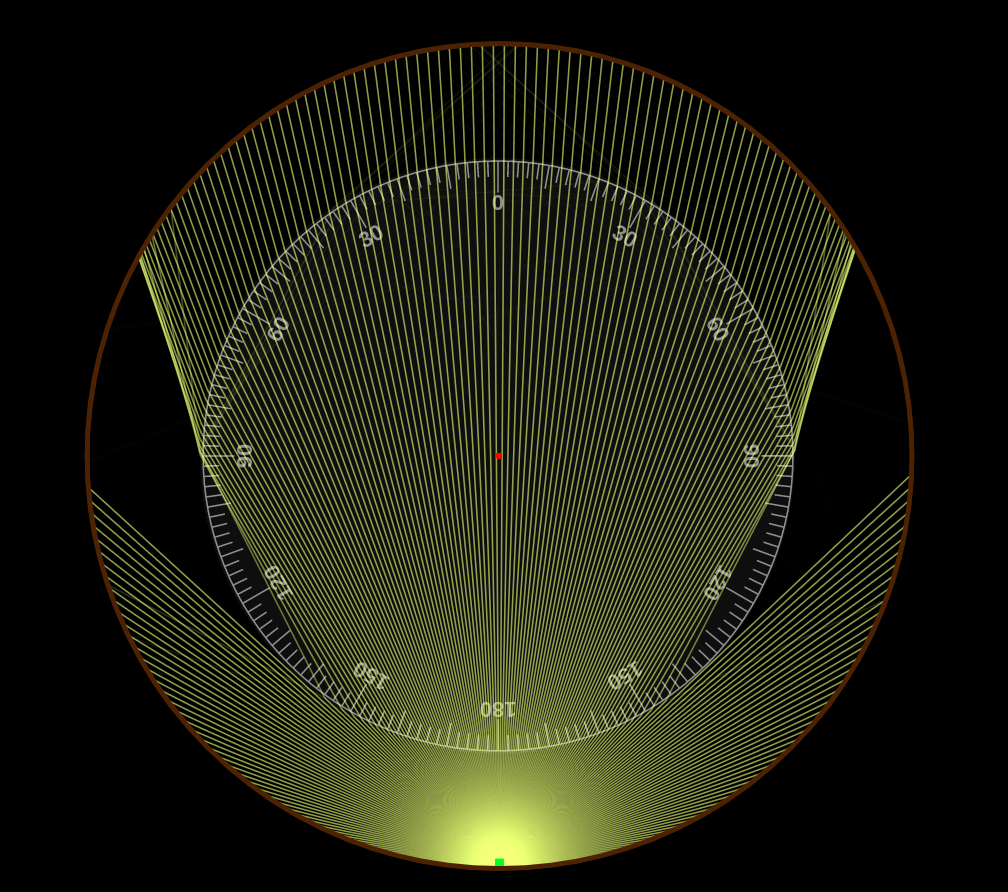
\includegraphics[width=0.8\textwidth]{5_SMELLIEAnalysis/images/smellie_scattering_region_ray_optics_model.png}
    \caption[Model of light rays propagating in the SNO+ detector during scintillator phase, emanating from an external source such as SMELLIE]
    {Model of light rays propagating in the SNO+ detector during scintillator phase, emanating from an external source such as SMELLIE. Because of refraction, a large ringed region is formed where no direct light can reach the region from the source. This forms the basis of the new scattering signal region.}
    \label{fig:smellie_propagation_toy_model}
\end{figure}

For this analysis, this new scattering signal region will be known as the ``bad light-path'' region, because no direct light-paths can be found. By consequence, it is impossible to calculate a time residual for hits in this region, as no direct light-path time-of-flight calculation is possible. Instead, times are calculated simply by $t = t_{\mathrm{hit}}-t_{\mathrm{emm}}$, where the usual $t_{\mathrm{med}}$ method is used for calculating the emission time.

In order to try and ensure that the bad light-path region really contained no contribution from direct light, SMELLIE simulations were performed for each fibre, and only PMTs in the forward hemisphere relative to the fibre that also observed no hits from direct light were chosen. % CONFIRM; add picture of this?

Fig.~\ref{fig:smellie_bad_lightpath_region_tracked} shows the time distribution of hits in the scattering signal region, split by the different components of a simulation, using the PQ495 through fibre FS055. As can be seen, in the $[-25,+30]\,\si{\ns}$ time window there is a large peak that is dominated by light scattered by the scintillator. It is this time window that is used in this analysis to isolate the scattered signal for all fibres. 

\begin{figure}
    \centering
    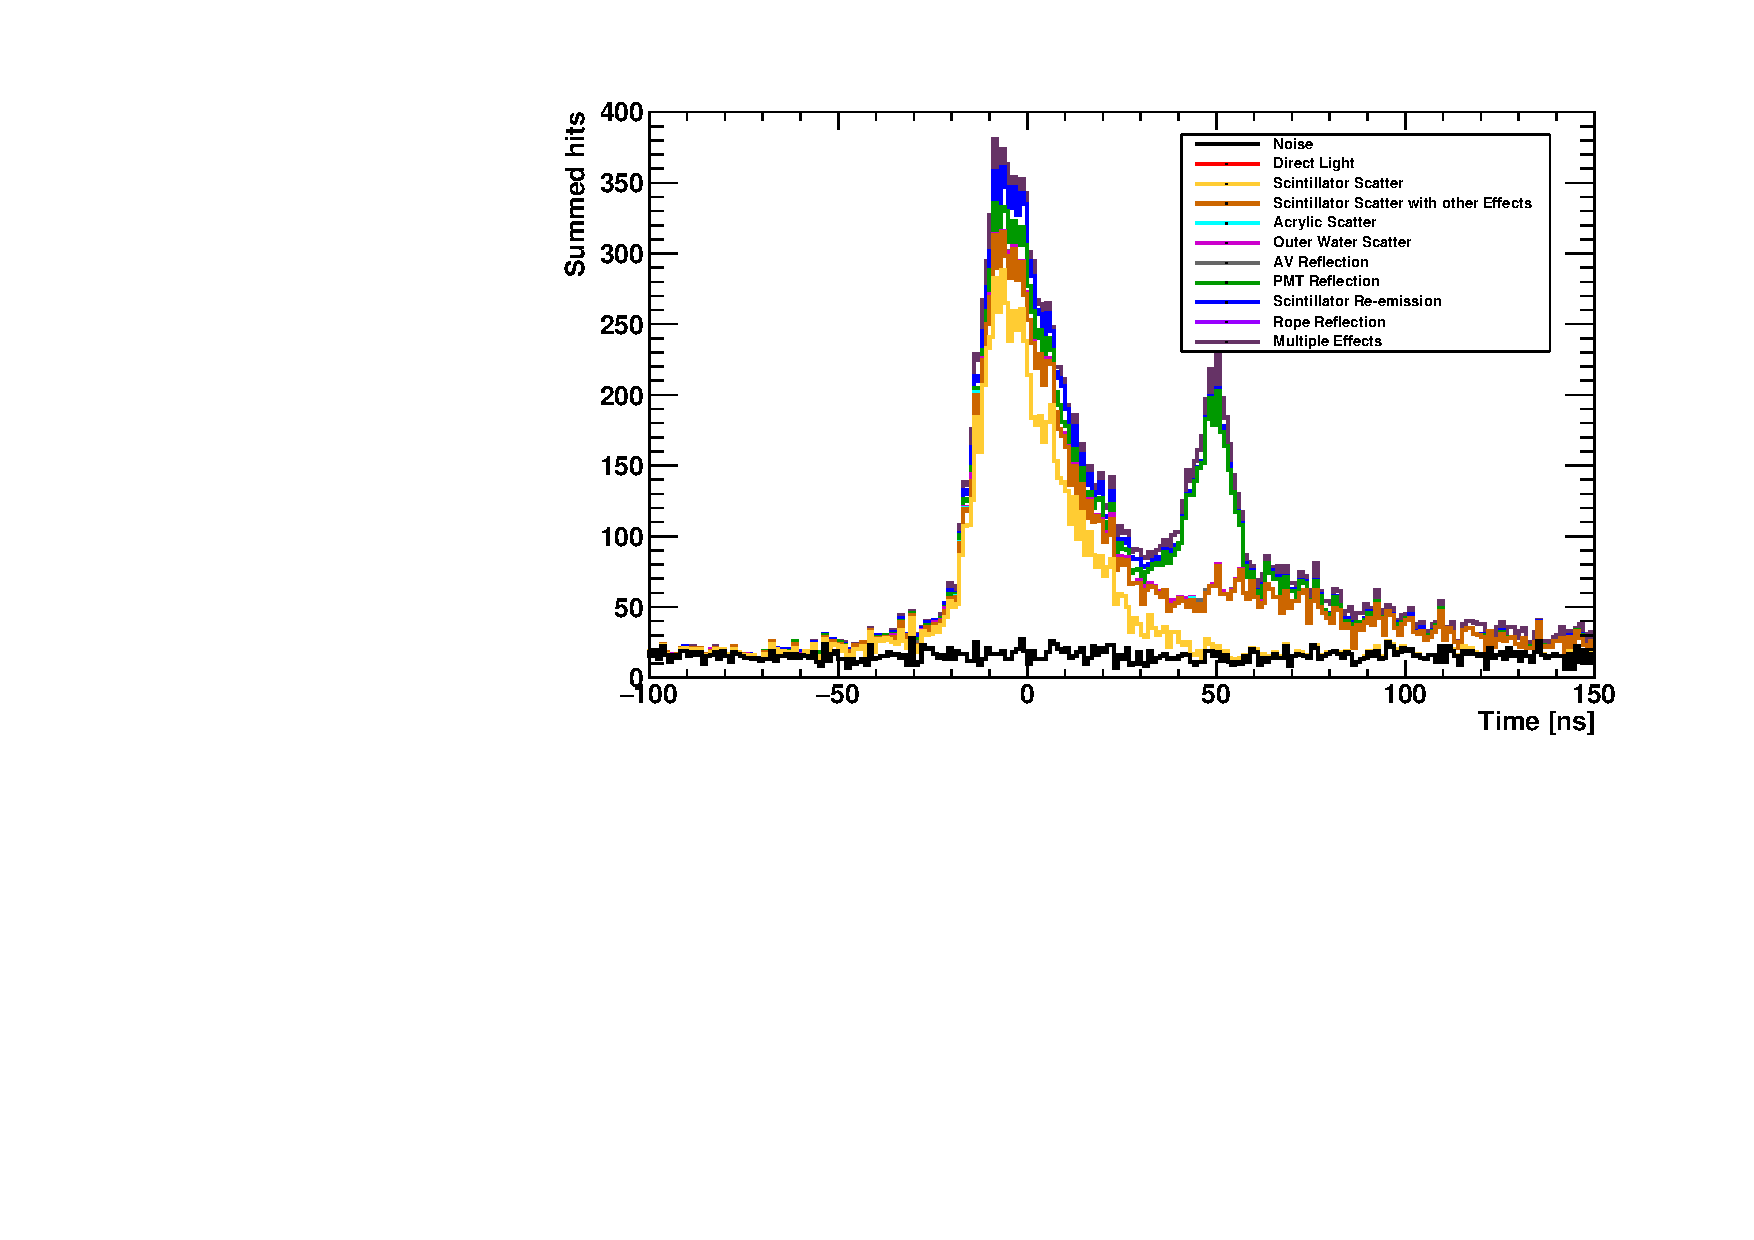
\includegraphics[width=\textwidth]{5_SMELLIEAnalysis/images/bad_lightpaths_components_plot_FS055_PQ495_Jul2022.pdf}
    \caption[Timing distribution of a simulation of the observed hits in the bad light-path PMT selection, split by optical components]
    {Timing distribution of a simulation of the observed hits in the bad light-path PMT selection through fibre FS055, using the PQ495 laser. The distribution is split into the different optical components.}
    \label{fig:smellie_bad_lightpath_region_tracked}
\end{figure}

In addition to having a high signal purity, this new scattered signal region has the benefit of being robust to beam profile uncertainties. Although beam profile systematics impact the intensity distribution of the direct light, no such light is seen in the signal region. Moreover, because scattered light must have a large scattering angle to reach the signal region, the beam profile shape is `washed out' by the scattering. As a demonstration of this effect, Fig.~\ref{fig:smellie_bad_lightpath_region_beamprofile_comparison} compares the observed time distribution in the bad light-path region for the new and old beam profiles of FS055, still using the PQ495 laser. One can see that there is little difference between the distributions a change of 1.0\% in the signal time window, compared to the more substantial differences seen in Fig.~\ref{fig:smellie_tres_alpha_data_mc}.

\begin{figure}
    \centering
    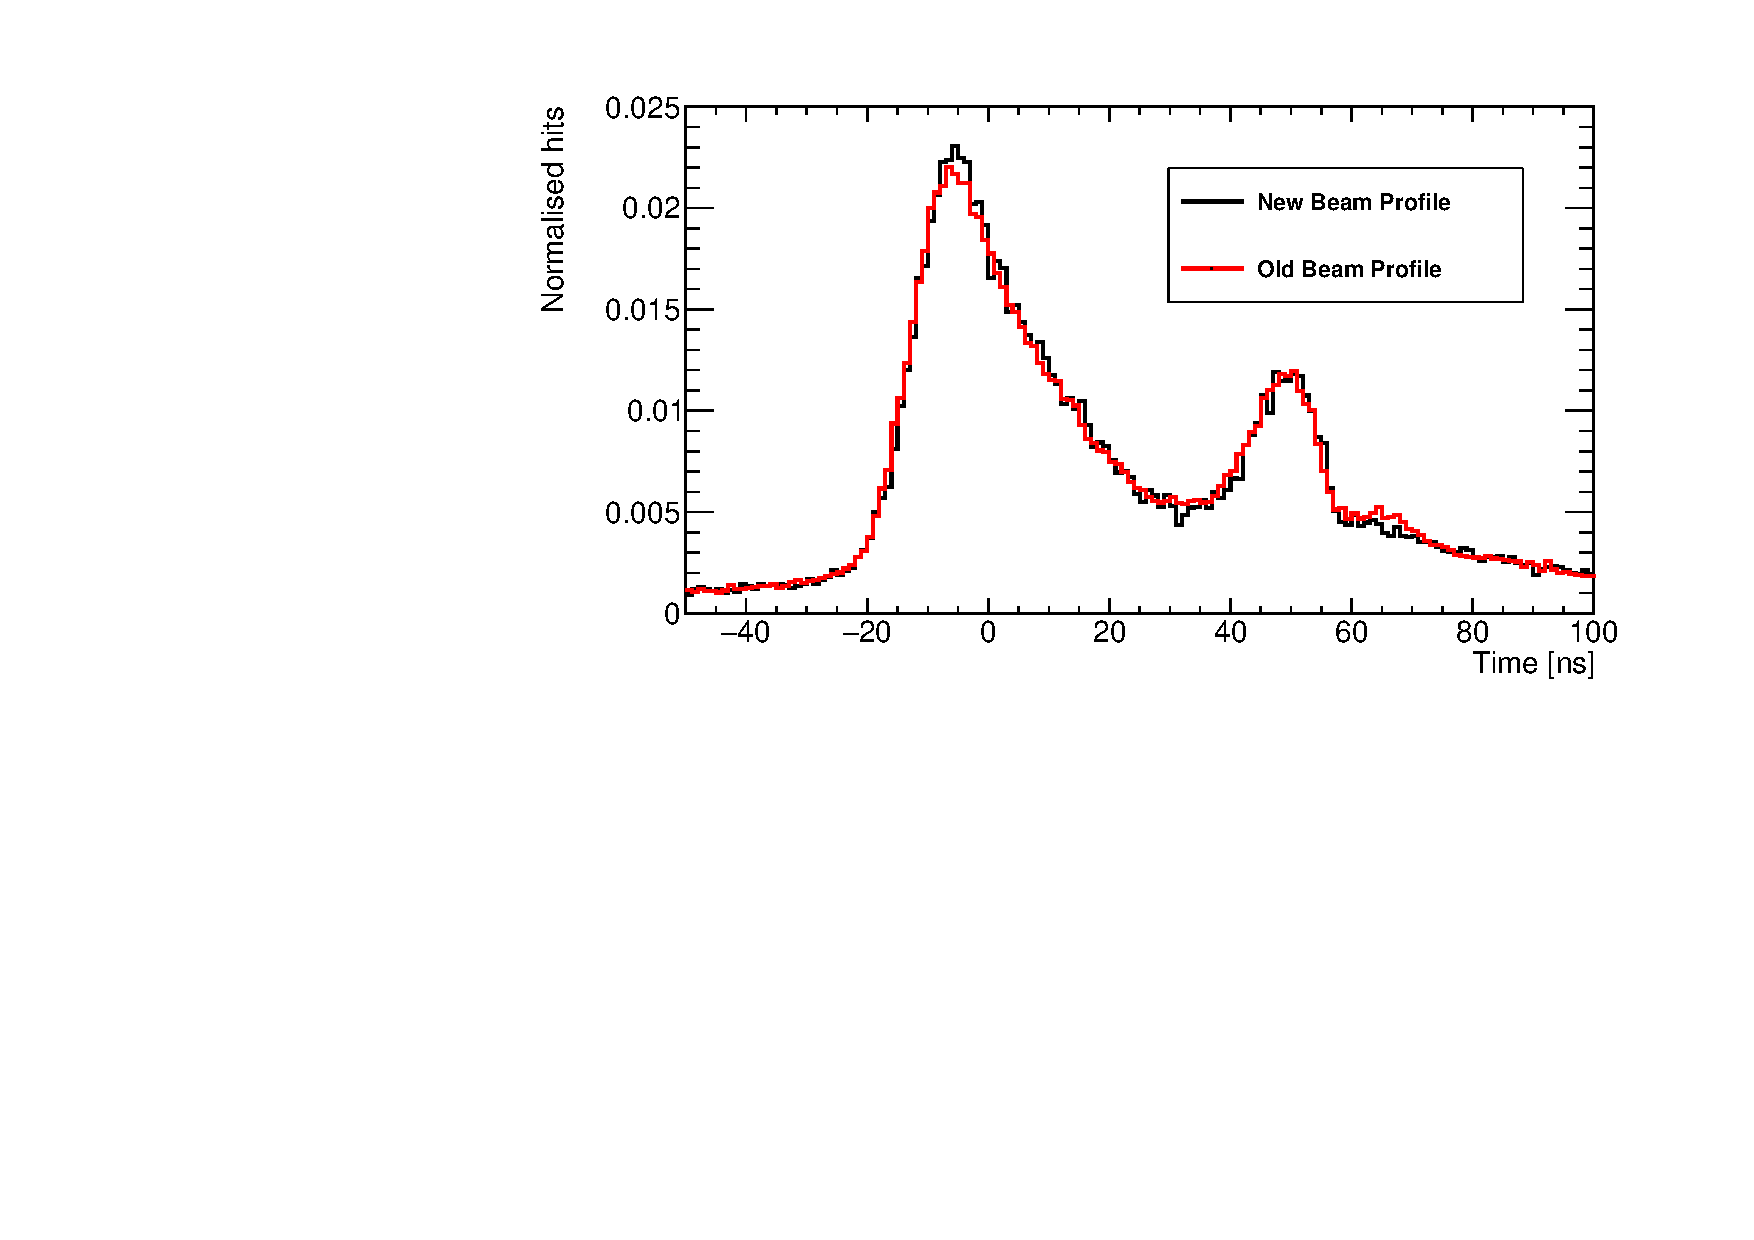
\includegraphics[width=\textwidth]{5_SMELLIEAnalysis/images/FS055_PQ495_new_vs_old_beam_profile_bad_lightpath_timeplot.pdf}
    \caption[]
    {Comparison of timing distributions in the bad light-path PMT region for simulations of laser PQ495 through fibre FS055, comparing the old and new beam profile. Both distributions have been normalised by the number of non-skipped events. The fractional difference in the number of hits in the signal time window is 1.0\%.}
    \label{fig:smellie_bad_lightpath_region_beamprofile_comparison}
\end{figure}

In the new signal region, some backgrounds to scattering are still present. These can come from PMT noise, scintillator re-emission, reflections off of PMTs and their concentrators, and combinations of multiple optical effects. A substantial fraction of the paths which undergo multiple processes scatter in the scintillator, and so are treated as signal for the purposes of this analysis. The contribution due to noise hits can be readily determined through the use of PULSEGT triggers, through the same approach used in Section~\ref{sec:smellie_ext_length_params_and_uncs}. In the example shown in Fig.~\ref{fig:smellie_bad_lightpath_region_tracked}, 82\% of non-noise hits in the signal region were from photons which underwent scattering in the scintillator.

\subsubsection{Observing Changes in Scattering}
If the absolute shot-to-shot intensity of a SMELLIE subrun is known, and the models of the scintillator re-emission and PMT reflections are well-enough known for the wavelengths of interest, then the scattering length of the scintillator can be determined by comparing data in the signal region to matching simulations of varying scattering length. Sadly, at the time of writing, no method for determining the absolute intensity which is sufficiently robust to systematic uncertainties in the modelling of MC is known. Instead, it was decided for this analysis to use the back-scattered light region described in Section~\ref{sec:smellie_ext_length_params_and_uncs} as a measure of relative intensity.

Without knowledge of the absolute intensity, absolute scattering lengths cannot be measured. However, by calculating the ratio of npe in the signal region to that of the back-scatter region for two equivalent scintillator subruns, denoted $R_{1}$ and $R_{2}$, any substantial change in the scattering length between datasets can be observed. Another restriction that this analysis has is that changes in the scattering length cannot be distinguished from changes in the background processes, in particular PMT reflections and scintillator re-emission. The reflectivity of the PMT concentrators is known to be changing slowly with time as the reflective petals of the concentrators degrade in the outer water~\cite{andersonOpticalCalibrationSNO2021}. % cite SNO, optics paper, Stringer thesis
The fractional change in their reflectivity over the course of the two-year period in which SMELLIE scintillator phase data was taken is expected to be XX\%, % CALCULATE!
assuming the same trends seen in SNO and the SNO+ water phase. Using the example shown in Fig.~\ref{fig:smellie_bad_lightpath_region_tracked}, 6.5\% of non-noise hits in the signal region came from PMT reflections, meaning that the overall systematic effect of concentrator degradation is expected to be merely XX\%. % CALCULATE!
 
The other dominant source of background is scintillator re-emission. This is expected to change as a function of PPO concentration. However, because the absorption length of the scintillator at \SI{2.2}{\gpl} is substantially longer than the scattering length in the \SIrange{400}{500}{\nm} range according to the current \texttt{RAT} model, the proportion of this background component is expected to be small: see Figs.~\ref{fig:cherenkov_scintillator_abs_emit_dist}~\&~\ref{fig:scattering_lengths_upw_labppo_current}. According to the simulation shown in Fig~\ref{fig:smellie_bad_lightpath_region_tracked}, 7\% of non-noise hits in the signal region come from scintillator re-emission. This contribution is expected to be somewhat larger at shorter wavelengths. As a result, fractional changes in the measured value of $R$, $\frac{\left|R_{1}-R_{2}\right|}{R_{1}}\lesssim 10\%$, cannot be reasonably distinguished between changes in scintillator re-emission or scattering.

% \begin{itemize}
%     \item Propose the new analysis approach: looking at light in the ``bad light-path'' PMT region. Define what this region is.
%     \item Give qualitative argument for why we expect this region to be robust to the beam profile systematics: dominated by the scattered signal as no direct light can make it here, and changes to beam profile should get ``smeared out'' after scattering.
%     \item Show how simulations indicate this should be a region with a very high purity of scattered light, and (assuming all else being equal) robust to beam profile uncertainties.
%     \item Confirm robustness of selected PMT region to uncertainties in AV offset and fibre position.
% \end{itemize}
% [5 pages]
% \subsubsection{Measuring the Emission Intensity}\label{sec:smellie_intensity}
% \begin{itemize}
%     \item Remaining systematics is now in the calculation of an average absolute emission intensity.
%     \item Show how various methods don't work particularly well: whole detector npe, beamspot npe, backscattered light npe, ``bad light-path'' PMTs but at later times. Explain why it goes wrong for each method.
%     \item Look at "beamspot but excepting the central bit": if that works well, then we can continue!
%     \item Otherwise, we'll have to live with measuring relative scattering lengths instead of absolute amounts, using the outer water back-scattering as a measure of the relative emission intensity.
% \end{itemize}
% [4 pages]

\subsection{Results in Data}
The datasets used in this scattering analysis are the subset of those described in Table~\ref{tab:smellie_ext_length_data} which were taken in the scintillator phase by the SuperK laser between \SI{400}{\nm} and \SI{500}{\nm}. Only three scintillator datasets had SuperK data taken: May 2021, May 2022, and June 2023. The npe ratio for the first dataset is denoted by $R_{1}$, and used as the baseline to compare to the later two datasets, denoted $R_{2}$.

Results from the same wavelength for the same dataset pair were combined onto a plot, as shown in Fig.~\ref{fig:smellie_scat_r1r2_plots}. Because far more hits are observed in the signal region compared to the backscatter light region for all subruns, the dominant source of statistical uncertainty in $R$ comes from the latter region. As a result, data points with large $R$ values had much larger uncertainties, because these corresponded to subruns with lower statistics in the backscatter light region. In order to account for the non-negligible uncertainties along both axes, the same fitting procedure from Section~\ref{sec:smellie_ext_length_results} was used. This found the best-fit line $R_{2} = m\cdot R_{1}$ for each plot with an associated uncertainty.

\begin{figure}
    \centering
    \begin{subfigure}{0.48\textwidth}
        \centering
        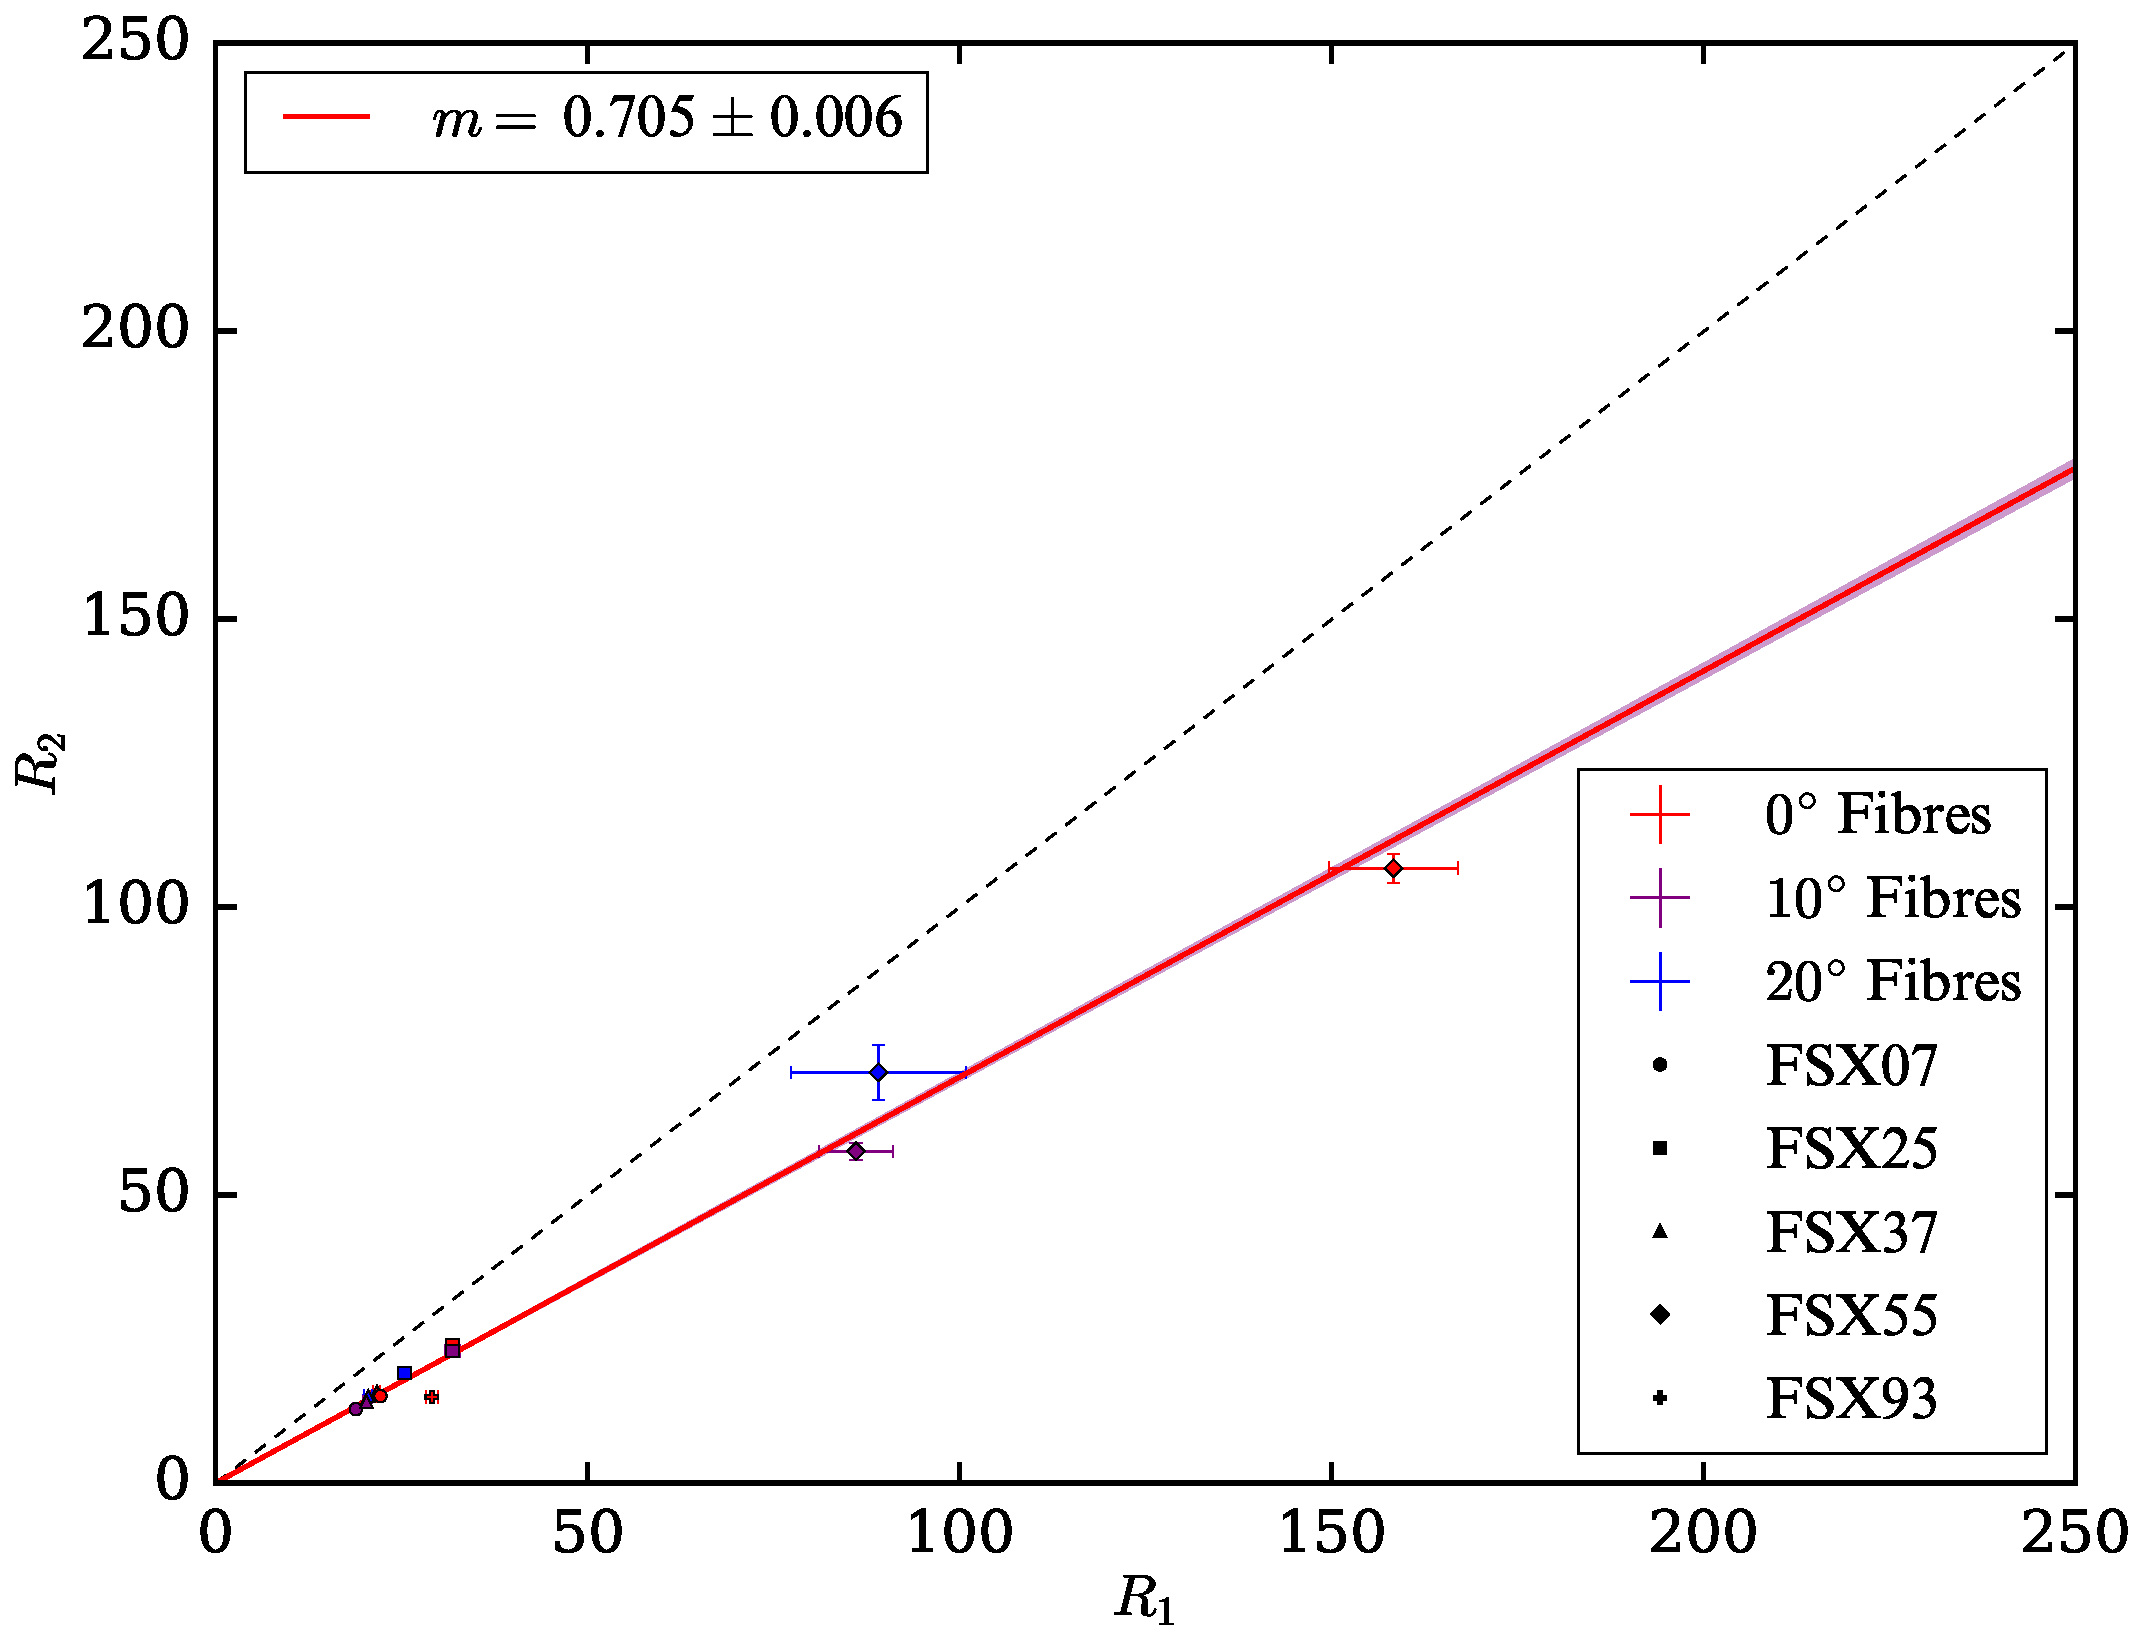
\includegraphics[width=\textwidth]{5_SMELLIEAnalysis/images/R1_vs_R2_superK_400_410_May2022.pdf}
        \caption{May 2021 versus May 2022, \SIrange{400}{410}{\nm}.}
        \label{fig:smellie_scat_r1r2_sk405_may22}
    \end{subfigure}
    \begin{subfigure}{0.48\textwidth}
        \centering
        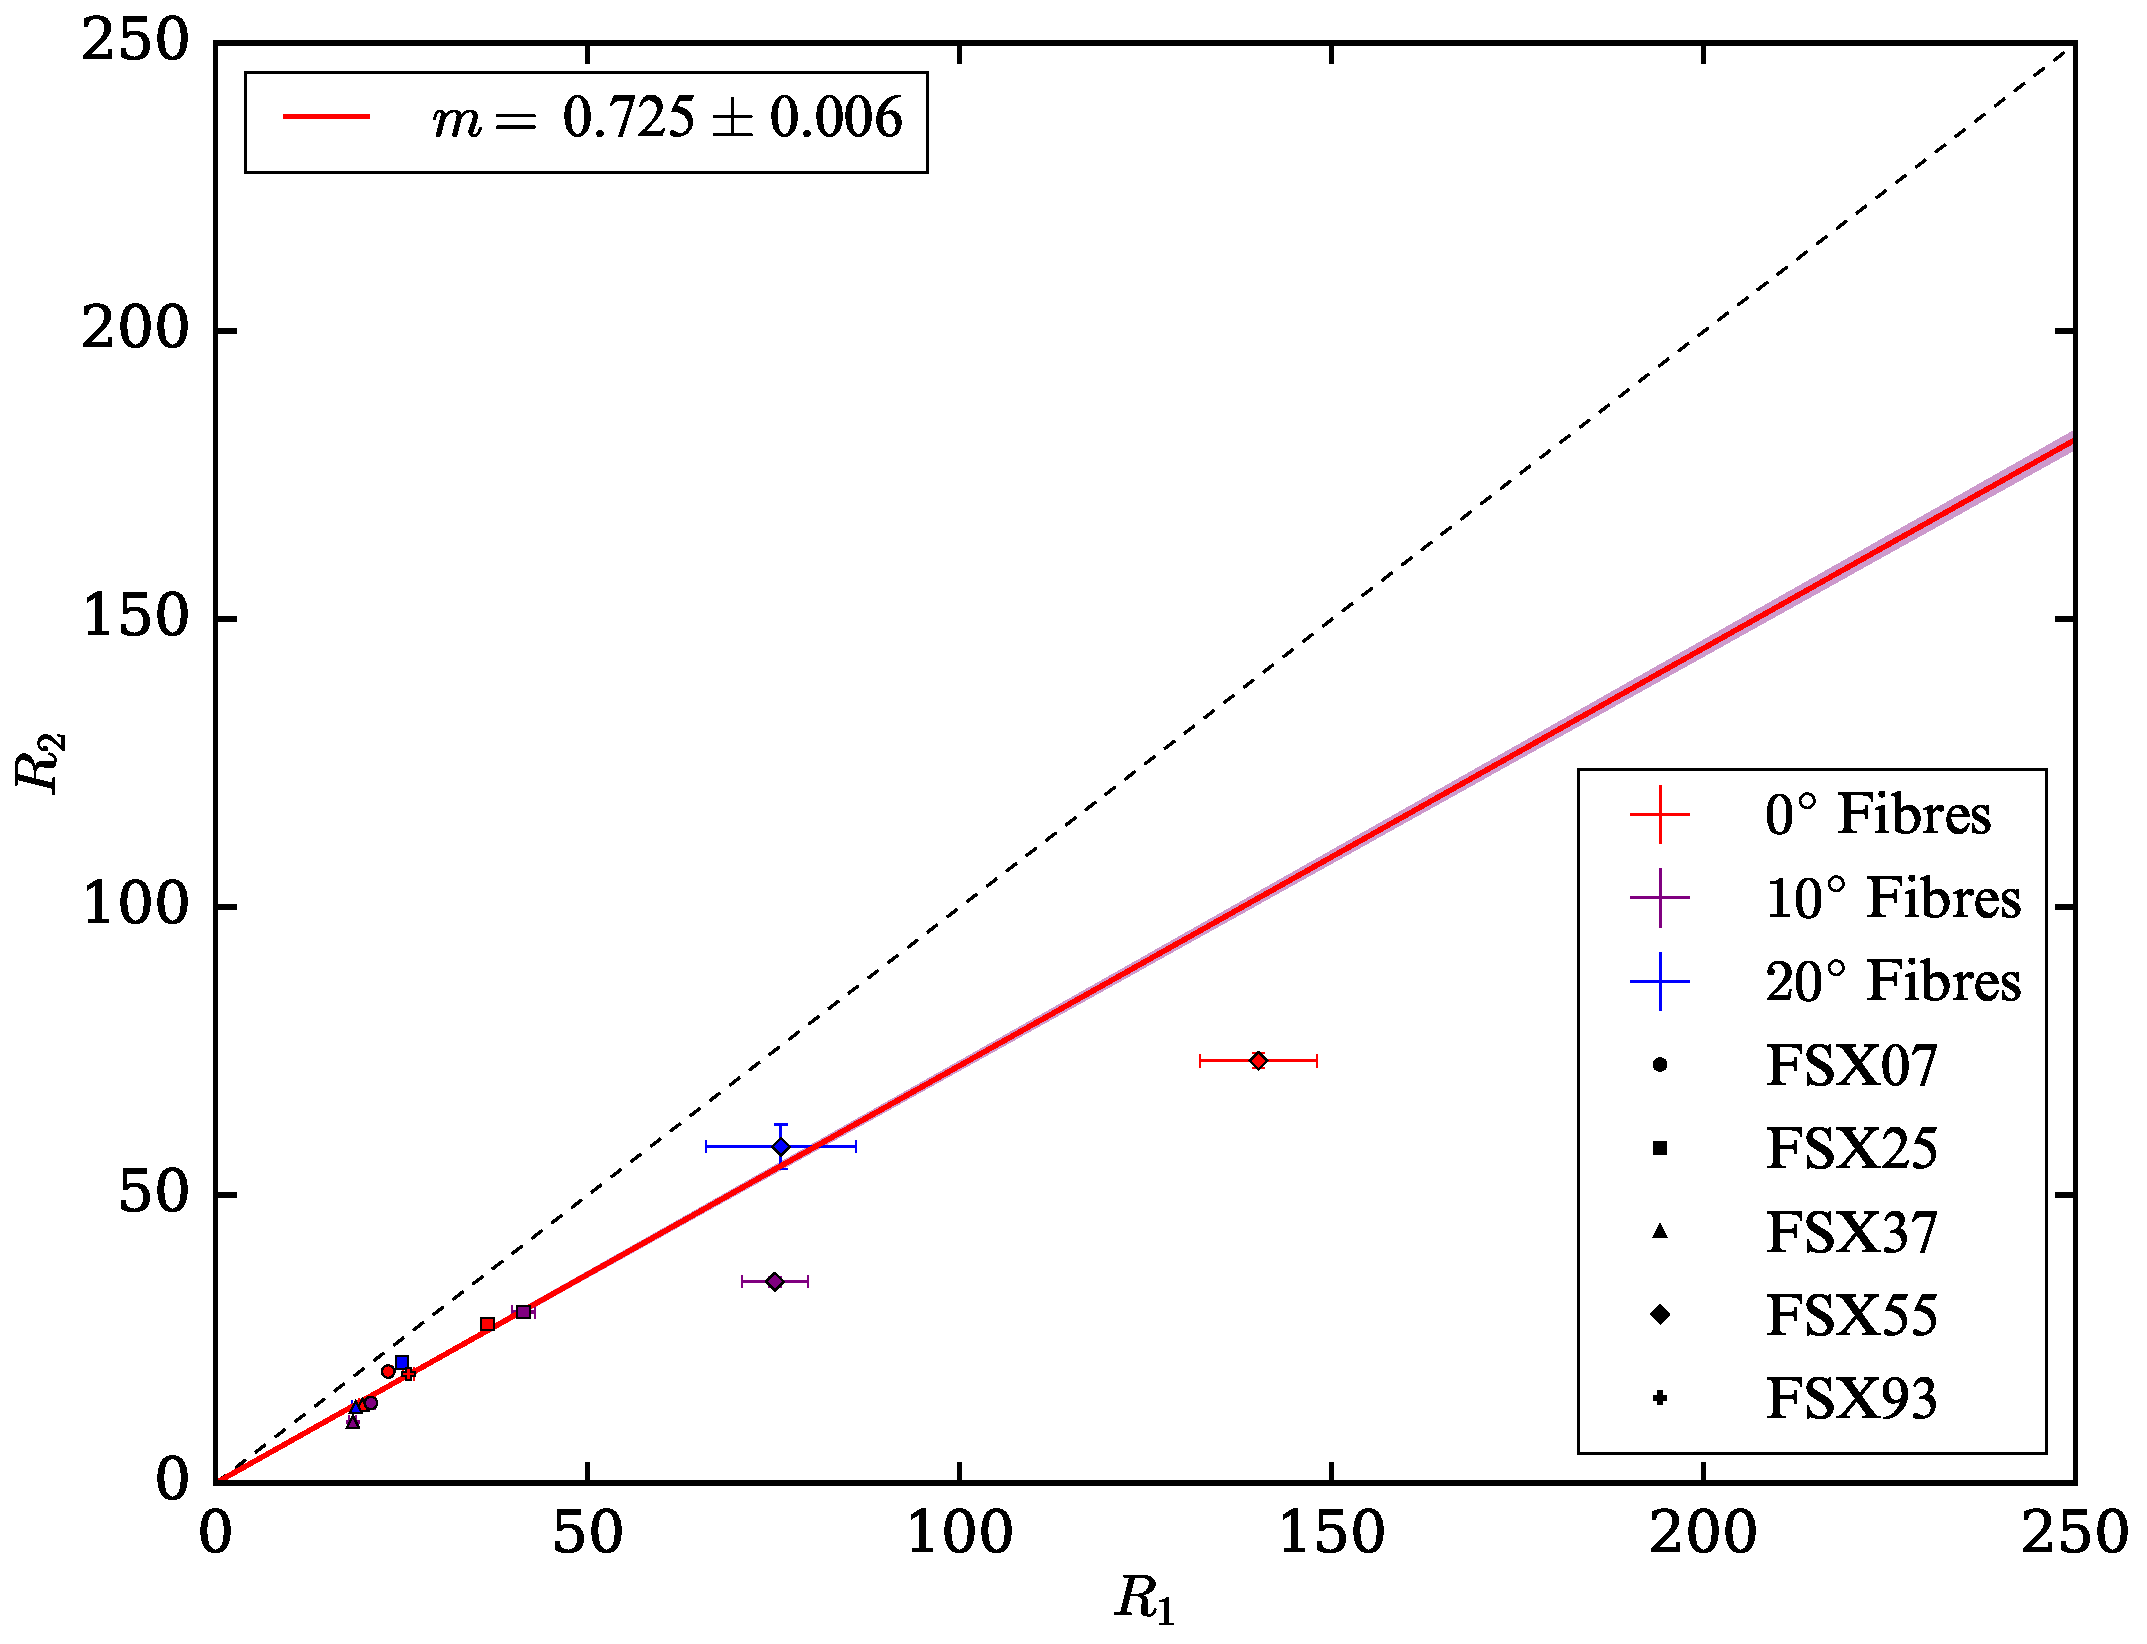
\includegraphics[width=\textwidth]{5_SMELLIEAnalysis/images/R1_vs_R2_superK_400_410_Jun2023.pdf}
        \caption{May 2021 versus June 2023, \SIrange{400}{410}{\nm}.}
        \label{fig:smellie_scat_r1r2_sk405_jun23}
    \end{subfigure}
    \begin{subfigure}{0.48\textwidth}
        \centering
        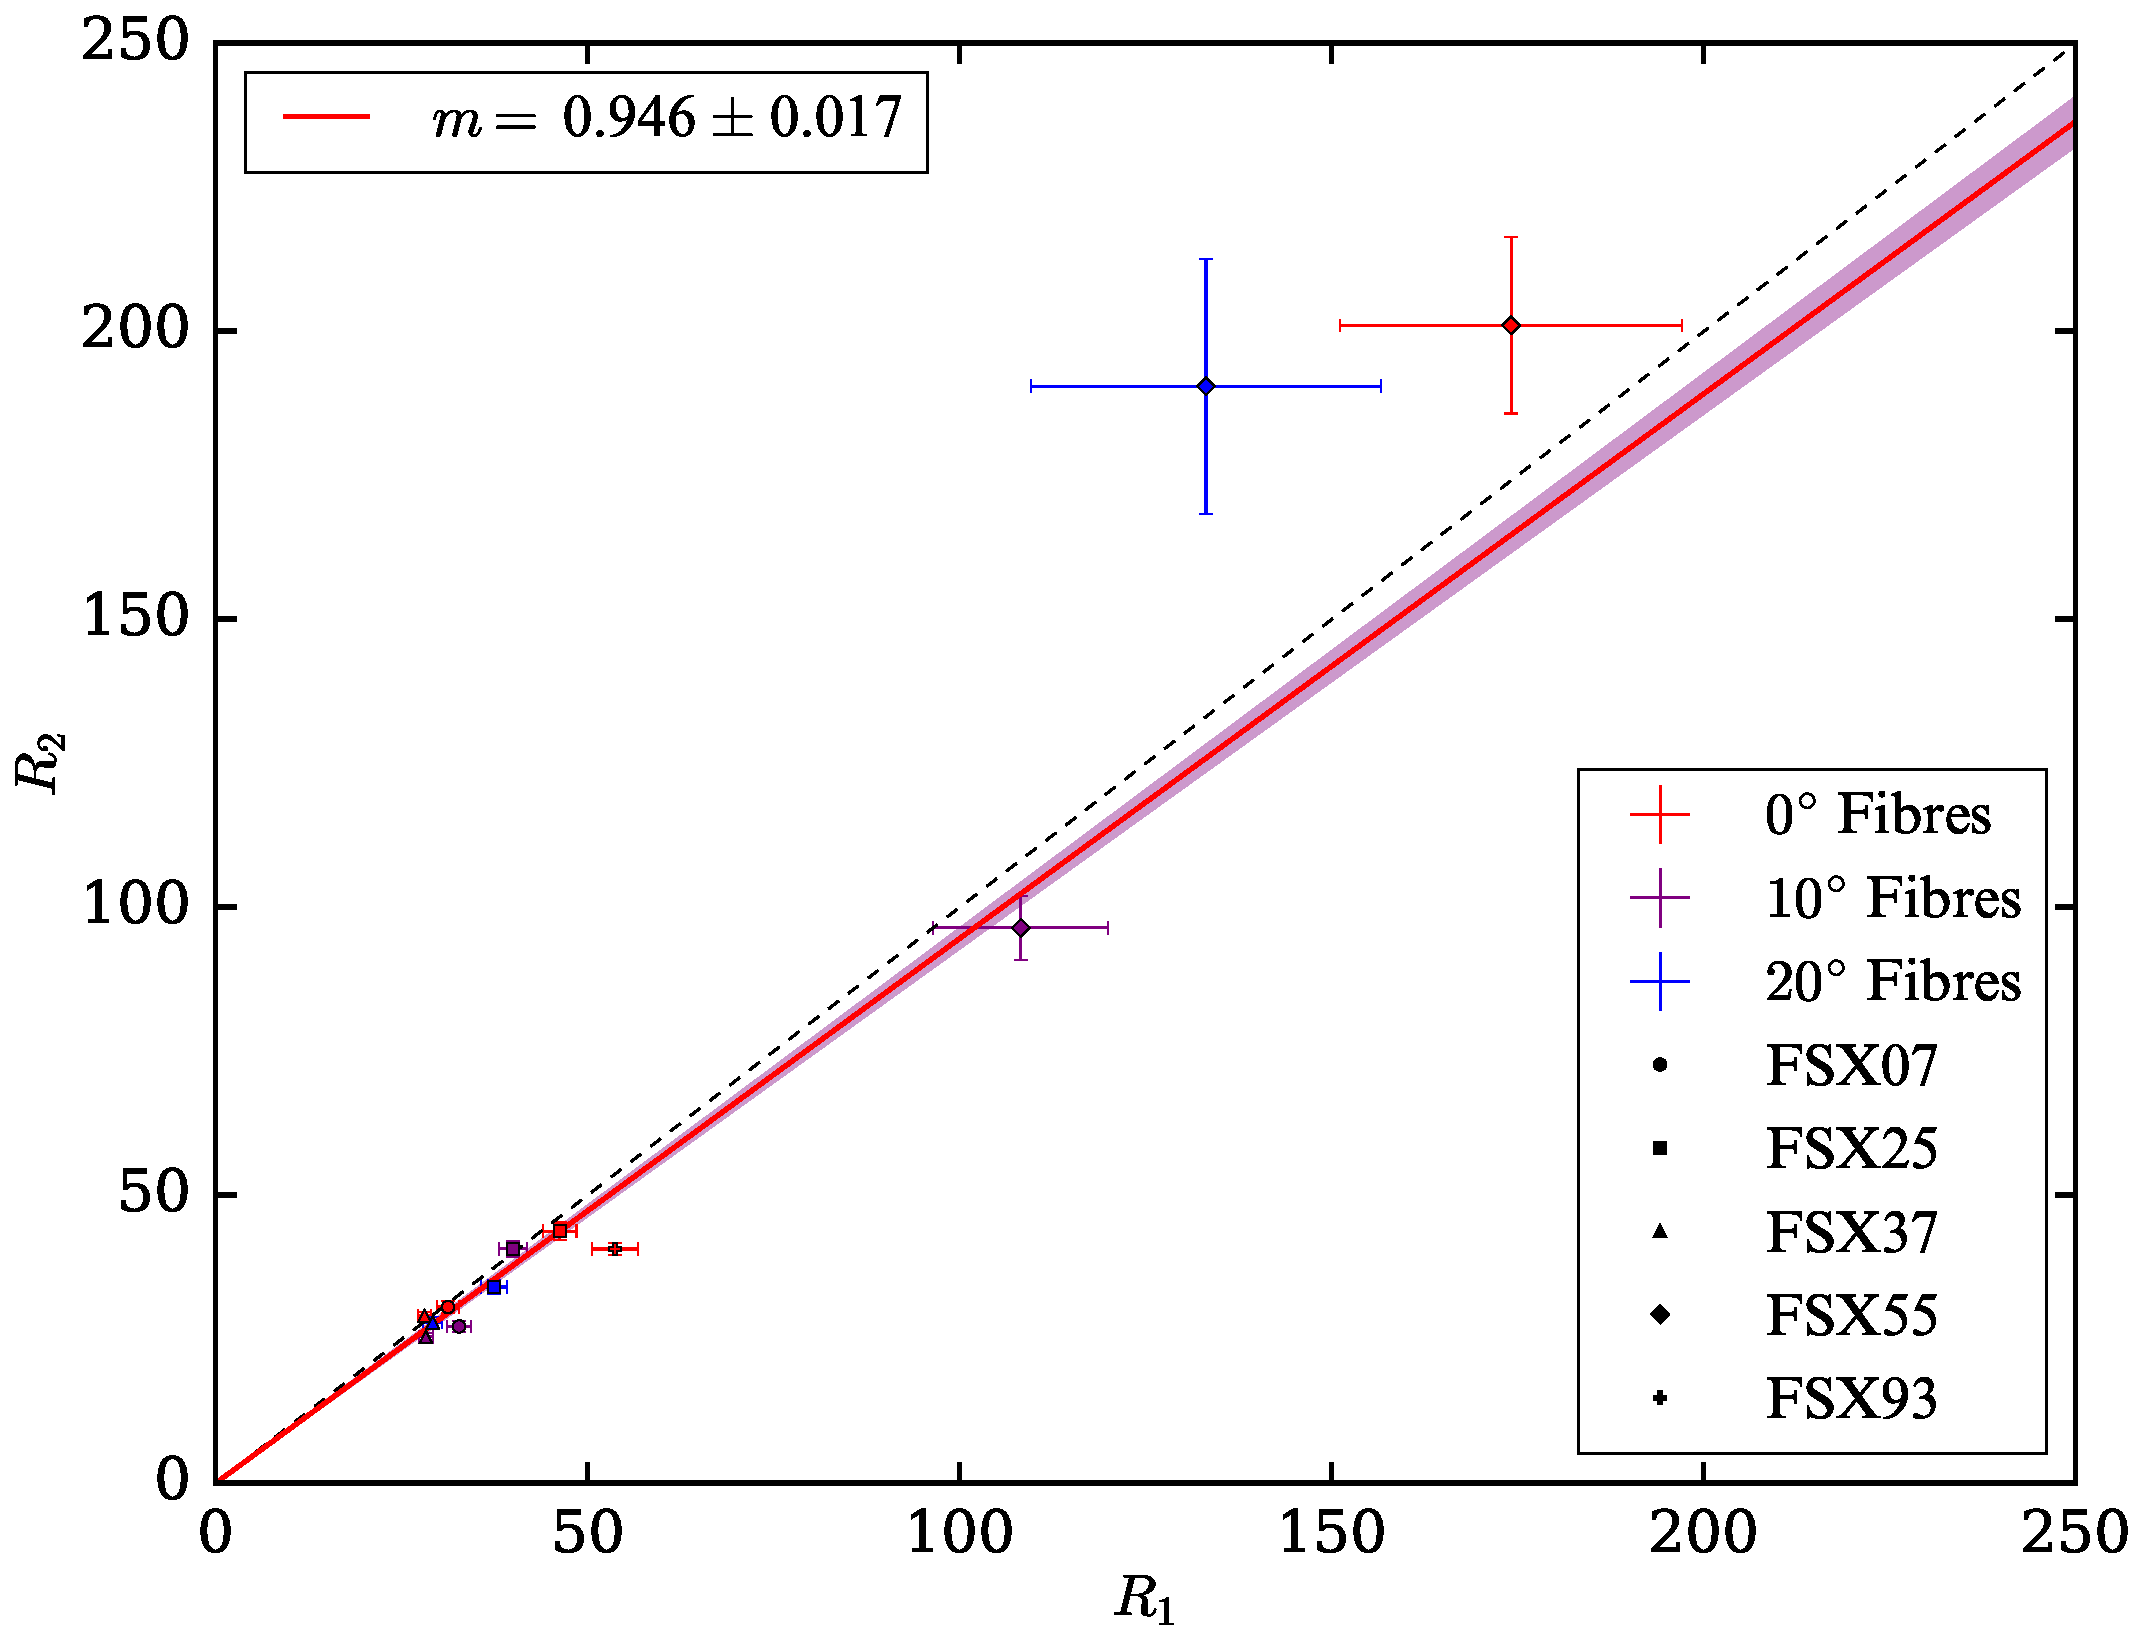
\includegraphics[width=\textwidth]{5_SMELLIEAnalysis/images/R1_vs_R2_superK_490_500_May2022.pdf}
        \caption{May 2021 versus May 2022, \SIrange{490}{500}{\nm}.}
        \label{fig:smellie_scat_r1r2_sk495_may22}
    \end{subfigure}
    \begin{subfigure}{0.48\textwidth}
        \centering
        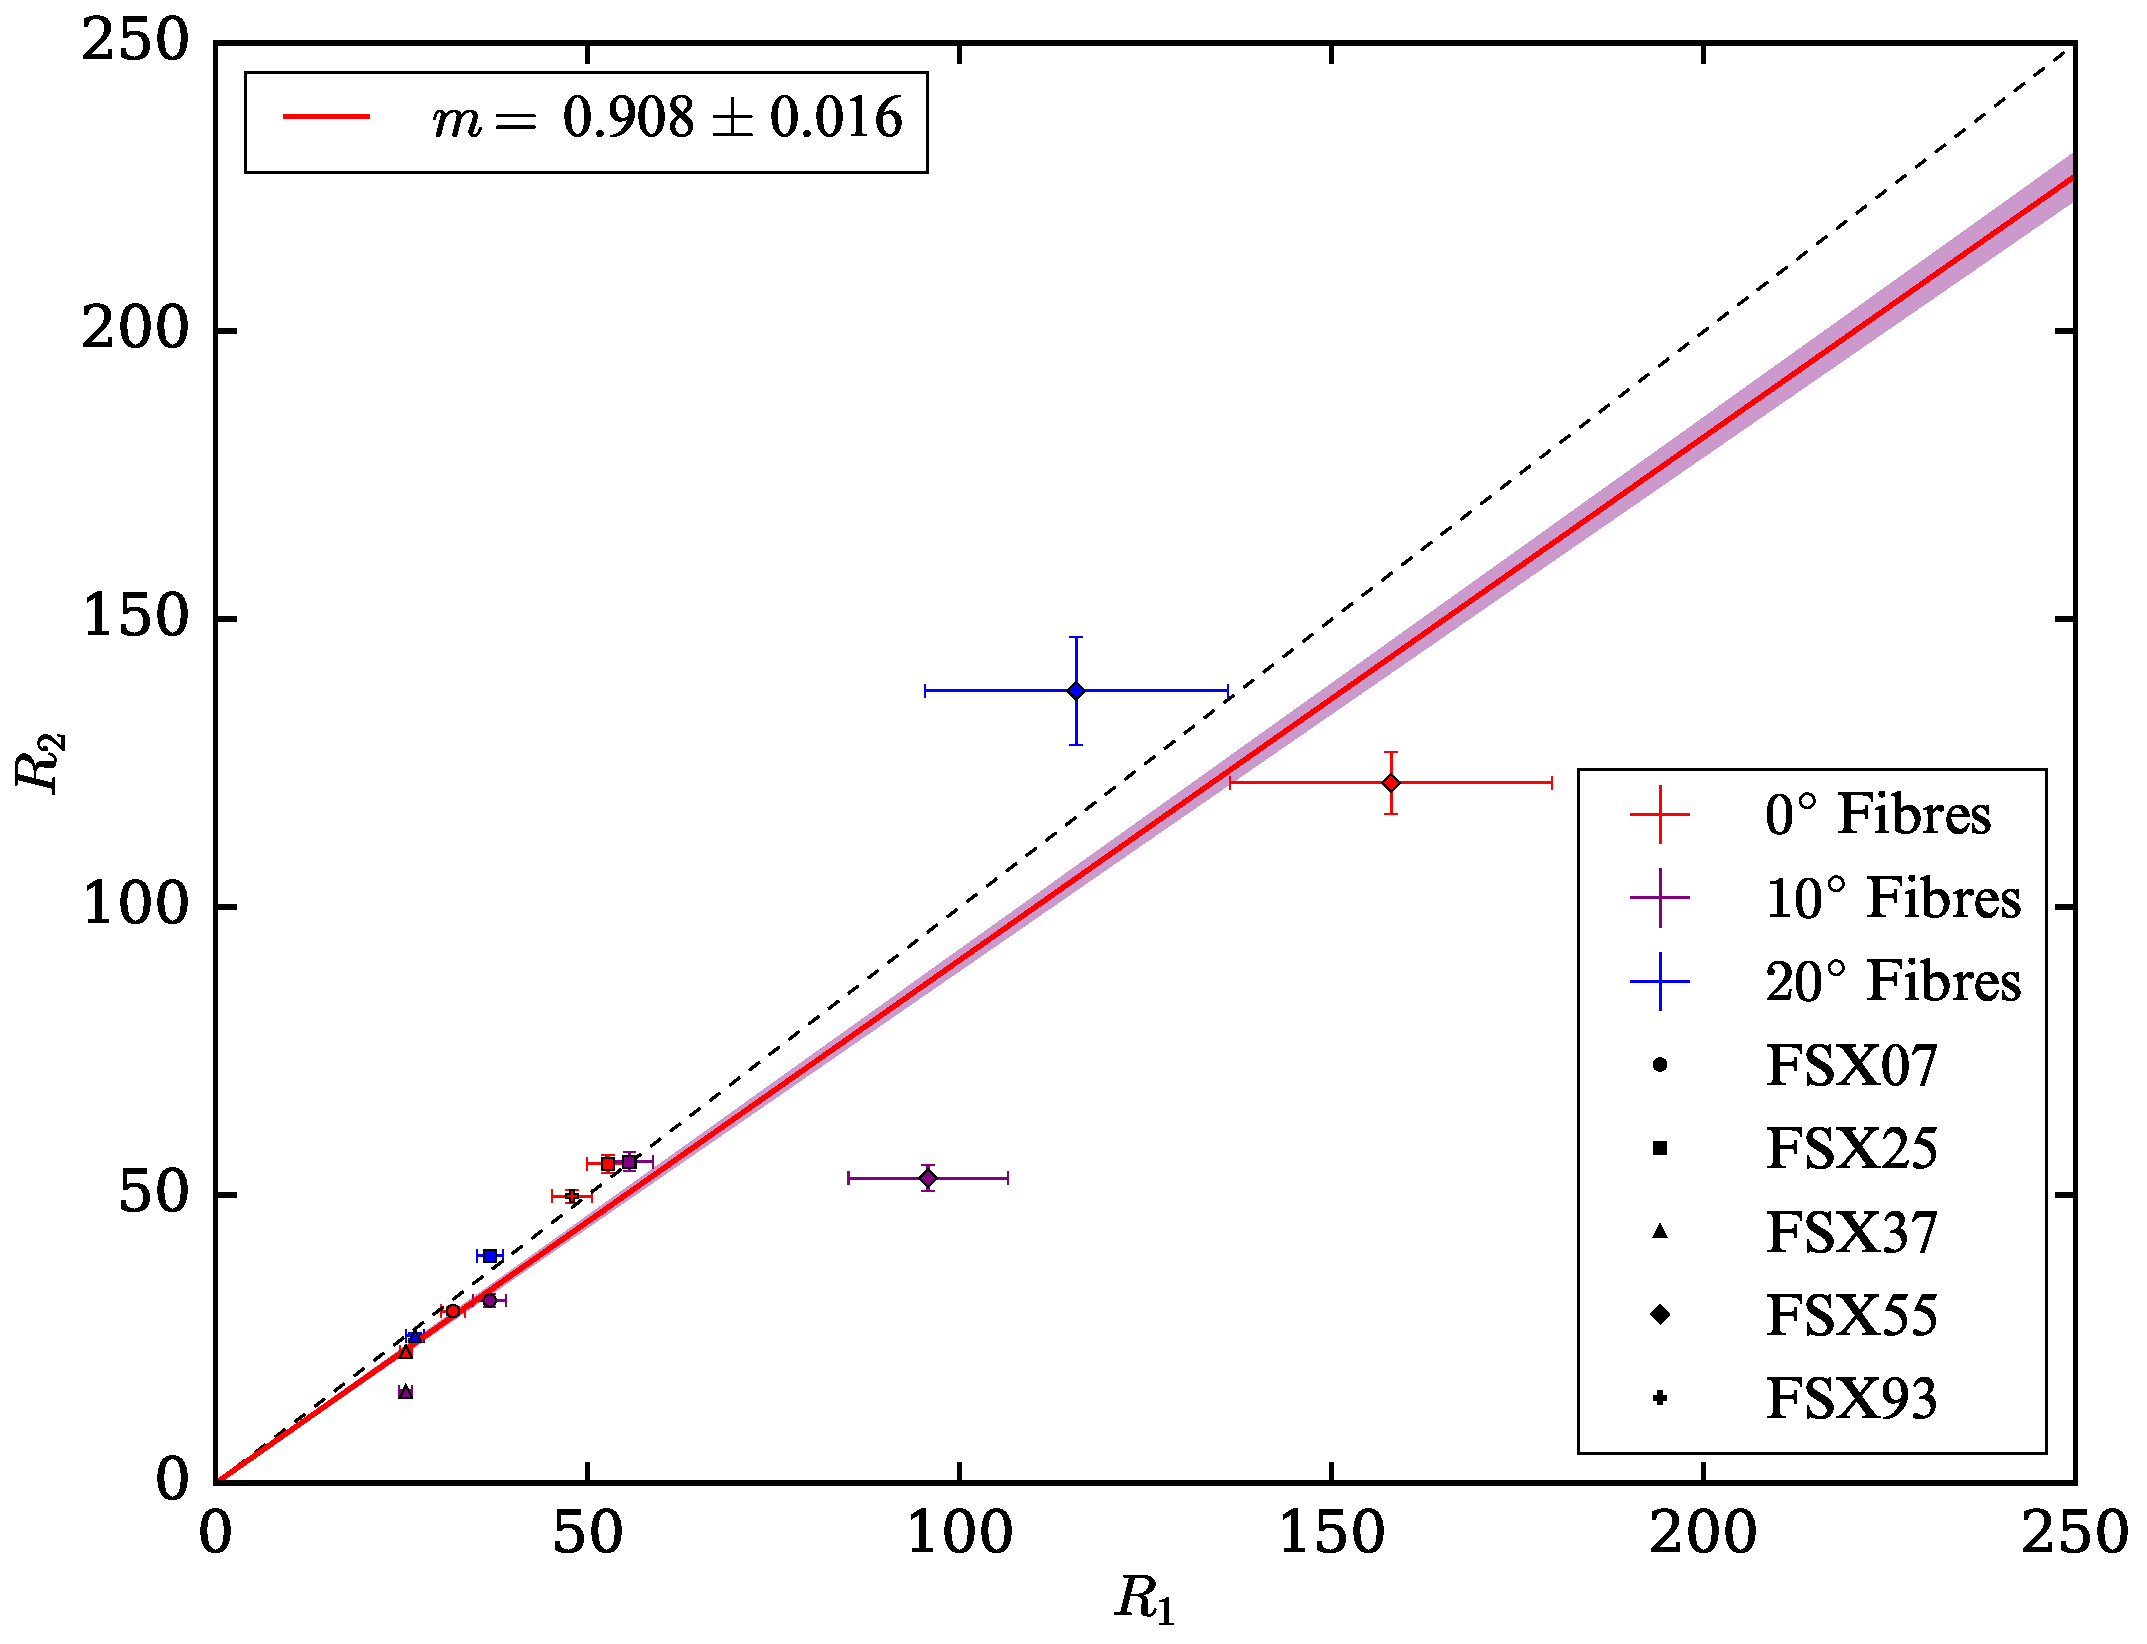
\includegraphics[width=\textwidth]{5_SMELLIEAnalysis/images/R1_vs_R2_superK_490_500_Jun2023.pdf}
        \caption{May 2021 versus June 2023, \SIrange{490}{500}{\nm}.}
        \label{fig:smellie_scat_r1r2_sk495_jun23}
    \end{subfigure}
    \caption[Plots of $R_{1}$ against $R_{2}$ for four pairs of scintillator phase datasets, using the SuperK laser]
    {Plots of $R_{1}$ against $R_{2}$ for four pairs of scintillator phase datasets, using the SuperK laser.}
    \label{fig:smellie_scat_r1r2_plots}
\end{figure}

The results for the gradient of all the data considered in this analysis are shown in Fig.~\ref{fig:smellie_scat_results_vs_wavelength}. All values for the ratio $R_{2}/R_{1}$ are found to be less than 1. This implies that, at all wavelengths in the range \SIrange{400}{500}{\nm}, less light was observed in the scatter signal region of the \SI{2.2}{\gpl} scintillator than the \SI{0.6}{\gpl} scintillator. Furthermore, there is a strong wavelength-dependence to this effect, such that shorter wavelengths observe a substantially lower fraction than at longer wavelengths. These results appear consistent to within statistical uncertainties for both \SI{2.2}{\gpl} scintillator datasets considered.

\begin{figure}
    \centering
    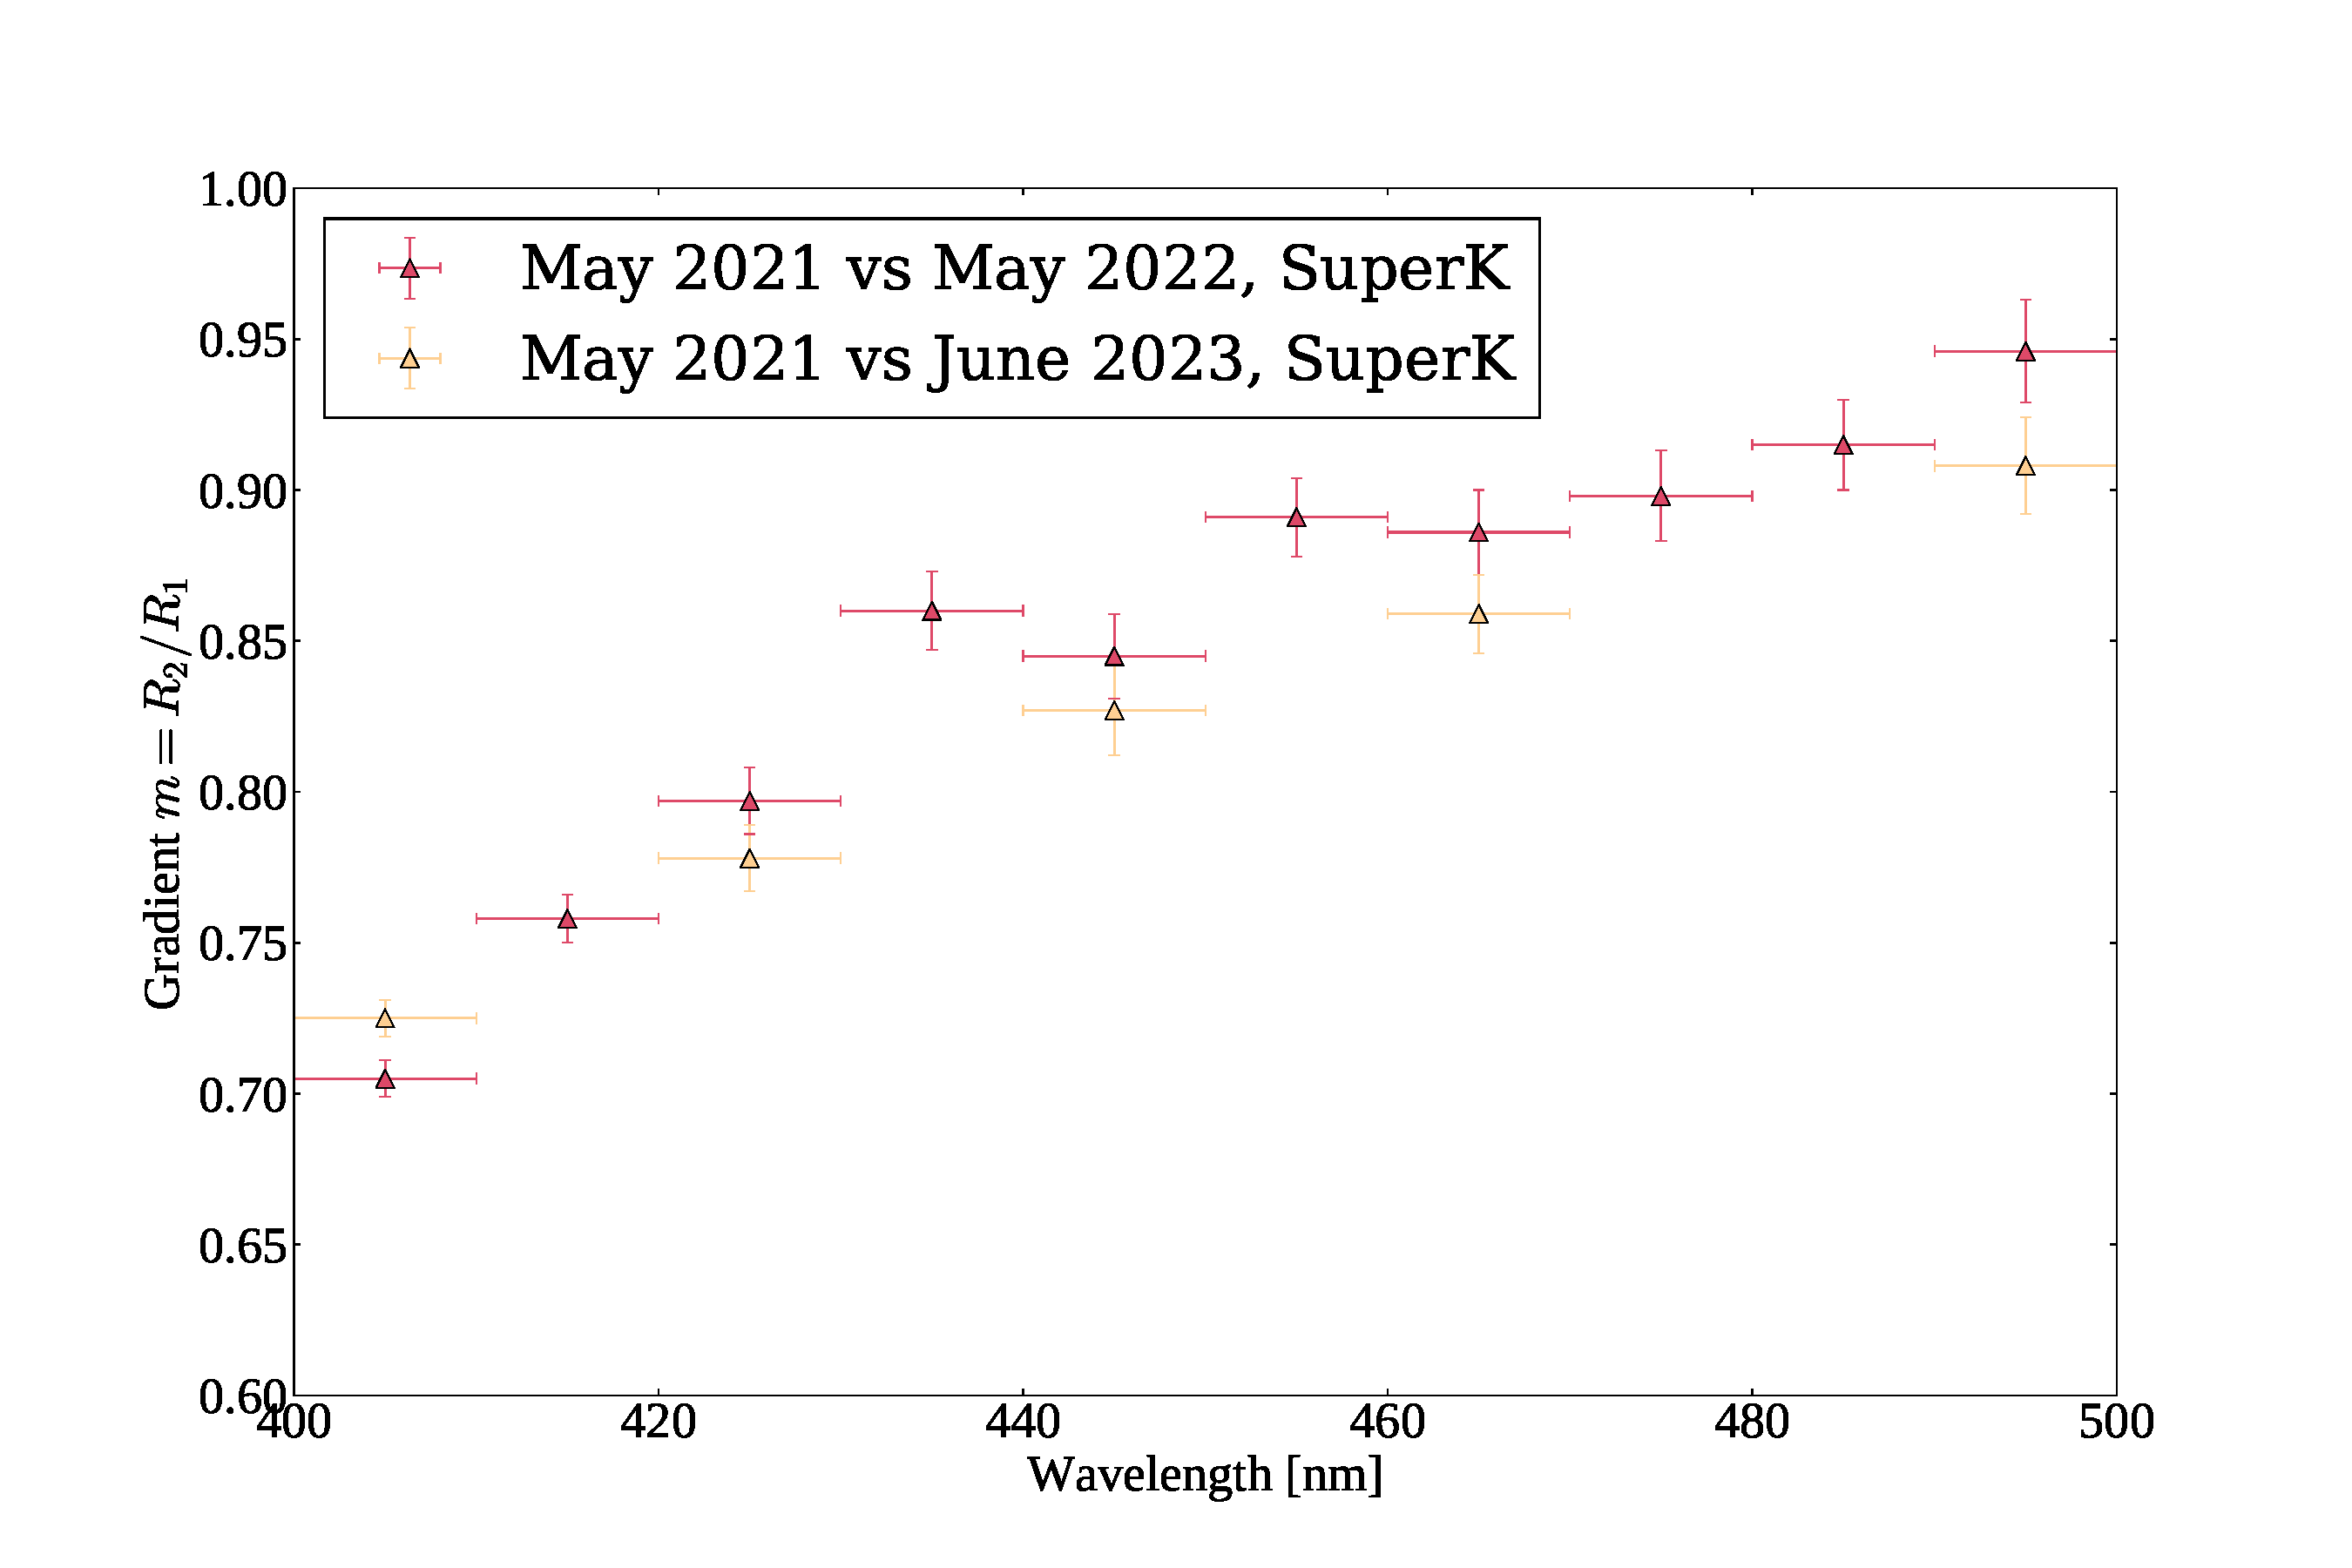
\includegraphics[width=\textwidth]{5_SMELLIEAnalysis/images/scattering_results_summary.pdf}
    \caption[Summary of results from the scattering analysis]
    {Summary of results from the scattering analysis, shown as a function of wavelength.}
    \label{fig:smellie_scat_results_vs_wavelength}
\end{figure}

\subsection{Interpretation}\label{sec:smellie_scat_discussion}
A na\"{i}ve reading of the above results would say that the scattering length has increased substantially between May 2021 and May 2022. However, that would be in strong tension with the results of the analysis of the previous section, which clearly shows a significant decrease in the observed extinction length over the same time period. It is also very difficult to explain from a theoretical perspective how the addition of PPO to the scintillator cocktail could decrease the amount of Rayleigh scattering.

There is an alternative interpretation which fits the observations of both analyses. Suppose that the scattering length did not change with time, but there was an additional non-re-emitting component of the scintillator added during the PPO loading. Then, this new component of the scintillator would be capable of absorbing light, shortening the observed extinction length, but the amount of re-emitted light could be much less than expectation in the wavelength range considered in this work. This would lead to a decrease in the amount of light observed in the scattered signal region, as the background re-emitted light substantially decreased in quantity. The expected fraction of light arriving in this region due to scintillator re-emission is, as seen in Section~\ref{sec:smellie_scatt_new_method}, of the correct magnitude to explain the change in the scattering signal region.

In the process of building the current \SI{2.2}{\gpl} scintillator absorption and scattering model, S. Riccetto and B. Tam found that adding a non-re-emitting absorption component was necessary to fit their calibration data simultaneously~\cite{kaptanogluDocumentationAttenuationStudies2022}. % cite 2.2 g/l model building
The origin of this new component was investigated by B. Tam, who concluded that near the end of the PPO top-up campaign some contaminants were likely added from the accidental overheating of the LABPPO during one of the distillation processes~\cite{}. % cite Ben's DocDB 7481; maybe thesis too?
There is a slight difference between their results and the implication from work in this thesis. S. Riccetto and B. Tam sought little evidence of this new component impacting longer wavelengths, and instead preferred causing a significant impact at short wavelengths $\lambda\lesssim\SI{400}{\nm}$.

\section{Summary and Suggestions for Future Work}
In this chapter, two analyses were developed and performed on data taken with the SMELLIE calibration system, to understand the optical properties of the scintillator within SNO+. The first analysis measured the extinction length of the scintillator as a function both of time and wavelength, through comparison to the already-calibrated water phase data. The extinction lengths found had some differences with existing models, although both see an increase the extinction length seen as a function of wavelength. A substantial decrease in the extinction lengths were observed between the May 2021 and May 2022, when the PPO concentration of the scintillator increased from \SI{0.6}{\gpl} to \SI{2.2}{\gpl}. However, the change in extinction length was far greater than the expected change to the absorption length of PPO. Data taken one year later, in June 2023, shows no indication of any further change to the scintillator's extinction length distribution.

In the second half of this chapter, another analysis was built, designed to be sensitive to changes in Rayleigh scattering. Simulations indicated that this new analysis was also sensitive to changes in the scintillator's  re-emission properties or changes in the PMT bucket reflectivity. By performing relative measurements between scintillator datasets, it was found that the amount of light seen in signal region decreased between May 2021 and May 2022, with similar results being seen when comparing May 2021 to June 2023 data. This could only be explained by a decrease in the quantity of scattered light, scintillator re-emission, or PMT reflections in the \SIrange{400}{500}{\nm} range. A significant wavelength-dependence was also seen in these results, with shorter wavelengths observing greater decreases in the amount of light seen.

The best physical explanation that combines these results is the existence of a new component of the scintillator cocktail that absorbs, but does not scatter or re-emit light substantially in the \SIrange{400}{500}{\nm} range. This would generate a significant shortening of the extinction lengths over these wavelengths, but decrease the amount of light seen in the signal region of the scattering analysis. This theory has similarities to the observations seen by B. Tam in ex-situ measurements, as well as the fits to the spectra of in-situ backgrounds performed by S. Riccetto. However, there remain some notable differences between my measurements and these others, in particular that there appears to be a non-negligble effect above \SI{400}{\nm}.

The key insight that enabled both of the analyses in this chapter is the building of analysis methods that were robust to the major systematics present in SMELLIE. By not comparing SMELLIE data to simulation, the discrepancies between the \texttt{RAT} model of SMELLIE and reality, described in Section~\ref{sec:smellie_systematics}, could be avoided. However, not using simulations in these analyses does come at a price. Firstly, the extinction length analysis becomes fundamentally dependent on the water phase data taken by both the Laserball and SMELLIE. The former had large systematic uncertainties in their UPW attenuation measurements that puts a firm limit on the precision that any extinction length measurement can make.

As an example, consider a measurement of the scintillator's extinction length at \SI{446}{\nm}, with a `true' value of the extinction length of \SI{12}{\m}. If the uncertainties from all other factors could be made negligible, because the derived attenuation length from the water Laserball data is \SI{108(49)}{\m}, this propagates to an uncertainty on the extinction length of the scintillator of 5\%. This effect becomes even larger as the extinction length increases.

This limitation is further compounded by the limited statistics taken in the SMELLIE water phase subruns used in this analysis. The extinction length analysis used `medium' intensity subruns, with the rare UPW backscatter light being used for intensity calibration, where for multiple PQ lasers there were very large shot-to-shot intensity variations. In addition, by needing to determine the emission time for each event independently, instead of being able to rely on the EXTA trigger timing, a small fraction of events may have leaked into or out of the time windows used in both analyses. This effect would be most predominant in data with a low number of hits in the beamspot region.

The other major source of uncertainty in the results of both analyses comes from the scatter between fibres around the line of best fit for a given plot. For example, in Fig.~\ref{fig:smellie_scat_r1r2_sk495_jun23} one of the points with the strongest pull on the fit value of the gradient is the purple triangle associated with fibre FS037. The backscattered light distributions that give rise to this data point are shown in Fig.~\ref{fig:smellie_FS037_backscat_tres_comparison}. As can be seen, there is a prominent change of shape of the peaks near $\tres{} = \SI{0}{\ns}$, which appears to leak into the backscattered light time window. The origin of this shape change is not yet known, but only appears to affect a few fibres in the most recent scintillator dataset. % confirm?
This problem could have minor impacts on the particular fit values which use this data, but all the qualitative results of this chapter would remain. %not a fan of this.

\begin{figure}
    \centering
    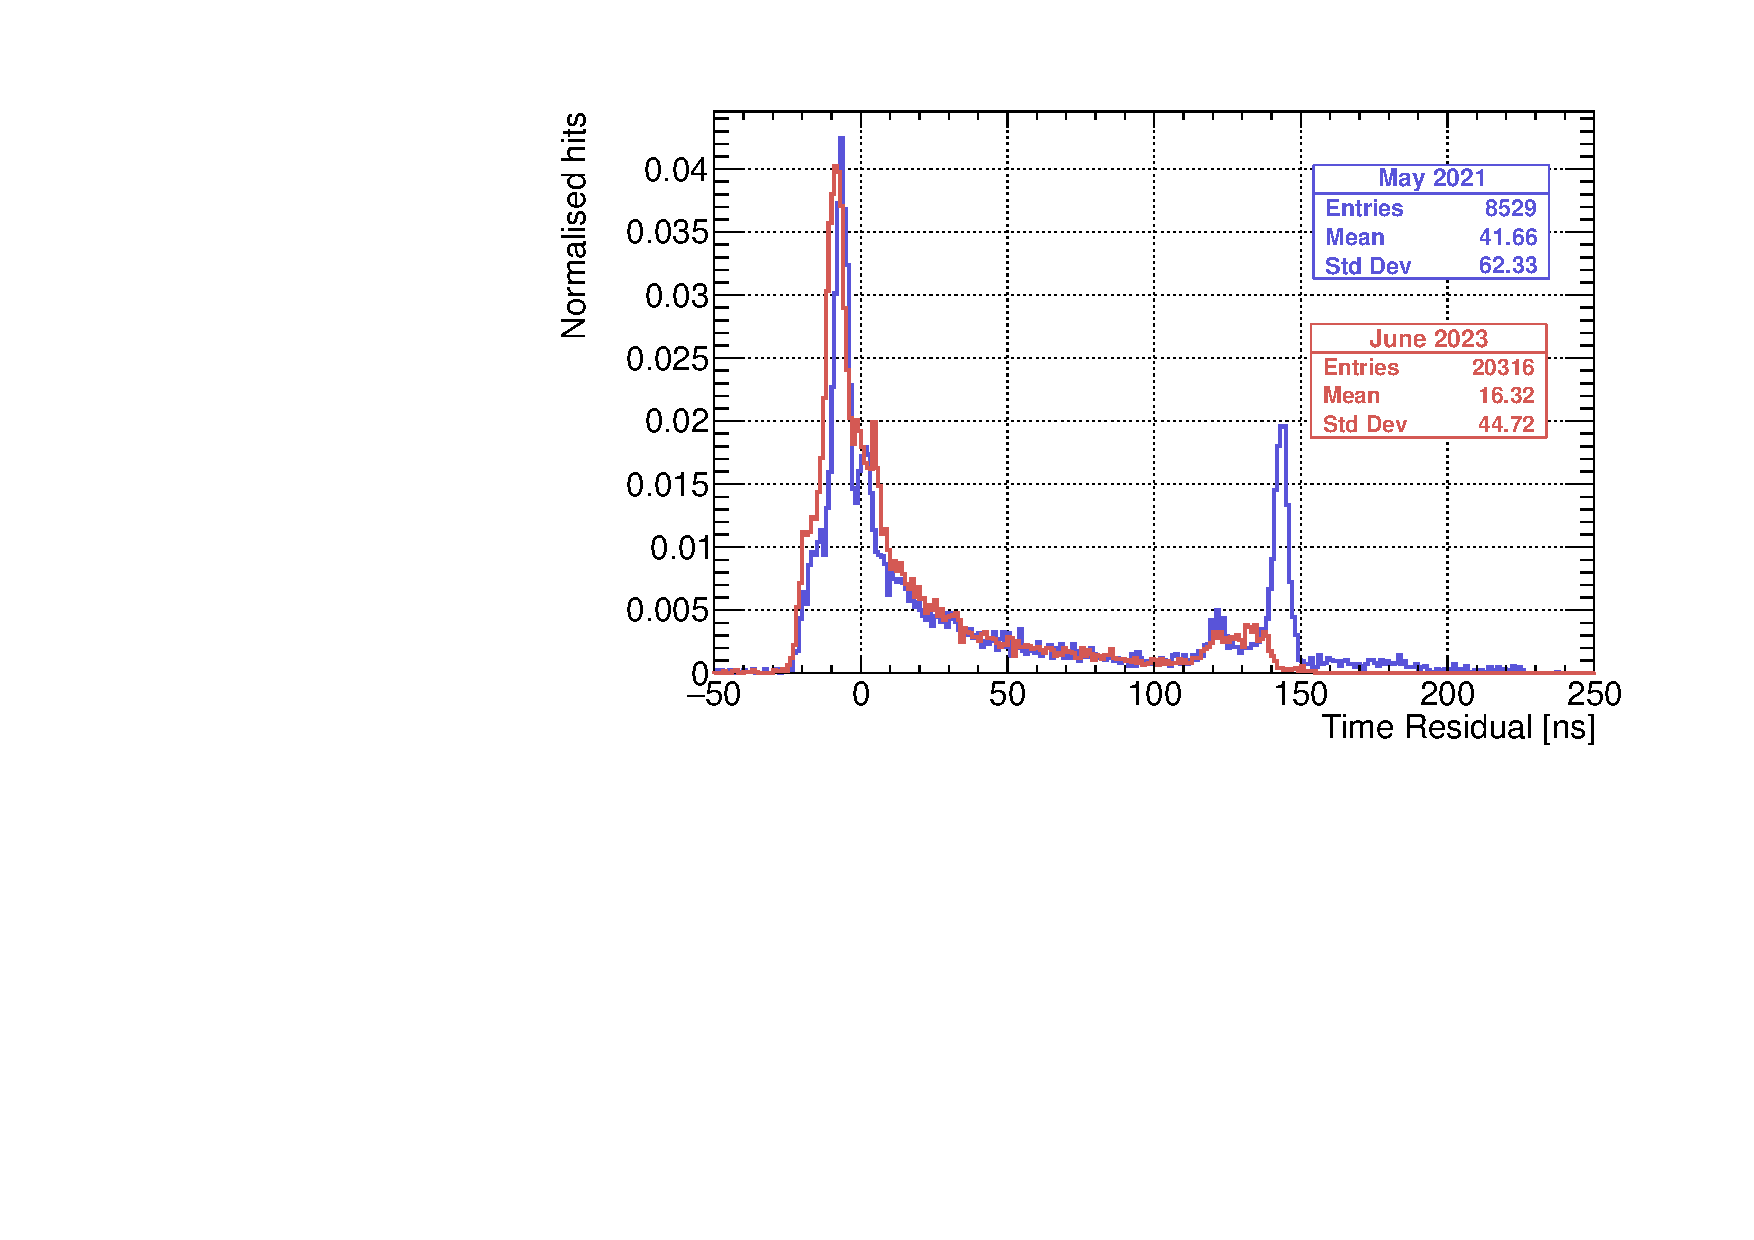
\includegraphics[width=\textwidth]{5_SMELLIEAnalysis/images/FS037_superK_490_500_May2021_vs_Jun2023_back_tres.pdf}
    \caption[Observed time residual distributions for the backscattered light region for FS037, comparing May 2021 to June 2023 data]
    {Observed time residual distributions for the backscattered light region of PMTs, with the SuperK laser in the \SIrange{490}{500}{\nm} range through fibre FS037. The distributions from both May 2021 and June 2023 are compared, with both of their distributions normalised to 1.}
    \label{fig:smellie_FS037_backscat_tres_comparison}
\end{figure}

There are a series of improvements that can be made to these two SMELLIE analyses, based upon the comments above. Major progress could be achieved if a robust measure of a fibre's absolute emission intensity could be found. In so doing, measurements of the extinction lengths and scattering properties of the detector media could be made independent of Laserball data or having to make merely relative measurements. This could become even more powerful if the beam profiles of the fibres for different wavelengths could be known with sufficient precision.

Another important set of considerations that will need to be made in the future in order to make precision scattering length measurements is the calibration of the scintillator re-emission and PMT reflections. It is worth noting that the analysis of Section~\ref{sec:scattering_analysis}, despite being designed for measuring changes in scattering length in the scintillator, actually appears to have measured a change in the re-emission properties of the scintillator. The impact of PMT reflections over time can be constrained by isolating regions of PMTs and time for which there is high purity of reflected light, such as the peak seen at \SI{50}{\ns} in Fig.~\ref{fig:smellie_bad_lightpath_region_tracked}. Alternatively, these could be calibrated through a deployment of the Laserball during the scintillator phase.

A possible approach to disambiguating between re-emission and scattering in scintillator is through their different scattering angle distributions. Whilst the former emits light isotropically, Rayleigh scattering has the angular form $\left(1+\frac{1-\delta}{1+\delta}\cos^{2}\theta\right)$, as discussed in Section~\ref{sec:optical_processes}. To do this, a secondary measurement of the scattered and re-emitted light could be made in the far PMT region. Because it is known that it is this light which are the dominant backgrounds to the direct light for the extinction length analysis, the amount of this background light which enabled the \ang{10} and \ang{20} fibres to best line up with the fit results of the \ang{0} ones could be determined. Then, this amount could be compared to the amount seen in the bad light-path signal region. One expects a difference in the observed amounts of scattered and re-emitted light in these two regions, because of the anisotropy of the Rayleigh scattering. With the differing values of these two different datasets, one might be able to tease apart the individual contributions of scattering and re-emission, and hence measure both.

% {
% \color{blue}

% \begin{itemize}
%     \item Actually do the proposed analysis on data, versus time and wavelength. Do the results seem consistent between fibres? Are they sensible values?
% \end{itemize}
% [5 pages]
% [33 PAGES TOTAL]
% }